\documentclass[journal,12pt,onecolumn]{IEEEtran}
\usepackage{cite}
\usepackage{graphicx}
\usepackage{amsmath,amssymb,amsfonts,amsthm}
\usepackage{algorithmic}
\usepackage{graphicx}
\usepackage{textcomp}
\usepackage{xcolor}
\usepackage{txfonts}
\usepackage{listings}
\usepackage{enumitem}
\usepackage{mathtools}
\usepackage{gensymb}
\usepackage{comment}
\usepackage[breaklinks=true]{hyperref}
\usepackage{tkz-euclide} 
\usepackage{listings}
\usepackage{gvv}                                        
%\def\inputGnumericTable{}                                 
\usepackage[latin1]{inputenc} 
\usetikzlibrary{arrows.meta, positioning}
\usepackage{xparse}
\usepackage{color}                                            
\usepackage{array}                                            
\usepackage{longtable}                                       
\usepackage{calc}                                             
\usepackage{multirow}
\usepackage{multicol}
\usepackage{hhline}                                           
\usepackage{ifthen}                                           
\usepackage{lscape}
\usepackage{tabularx}
\usepackage{array}
\usepackage{float}
\newtheorem{theorem}{Theorem}[section]
\newtheorem{problem}{Problem}
\newtheorem{proposition}{Proposition}[section]
\newtheorem{lemma}{Lemma}[section]
\newtheorem{corollary}[theorem]{Corollary}
\newtheorem{example}{Example}[section]
\newtheorem{definition}[problem]{Definition}
\newcommand{\BEQA}{\begin{eqnarray}}
\newcommand{\EEQA}{\end{eqnarray}}
\usepackage{float}
%\newcommand{\define}{\stackrel{\triangle}{=}}
\theoremstyle{remark}
\usepackage{circuitikz}
\usepackage{tikz}
\title{EC: ELECTRONICS AND COMMUNICATION ENGINEERING}
\author{EE25BTECH11037 - Divyansh}

\begin{document}

\maketitle

\begin{enumerate}

\item The order of differential equation  $\frac{d^2y}{dt^2}$ + $\brak{\frac{dy}{dt}}^3$ + $y^4$ = $e^{-t}$ is
\begin{enumerate}
\begin{multicols}{4}
\item 1
\item 2
\item 3
\item 4
\end{multicols}
\end{enumerate}
\hfill $\brak{\text{GATE EC 2009}}$

\item The Fourier series of a real periodic function has only 
\begin{enumerate}
\item cosine terms if it is even
\item sine terms if it is even. 
\item cosine terms if it is odd.
\item sine terms if it is odd.
\end{enumerate}
Which of the following statements is are correct?
\begin{enumerate}
\begin{multicols}{4}
\item a and d
\item a and c
\item b and d
\item b and c
\end{multicols}
\end{enumerate}
\hfill $\brak{\text{GATE EC 2009}}$

\item A function is given by $f(t)$ = $\sin^2t$ + $\cos2t$. Which of the following is true ?

\begin{enumerate}
    \item $f$ has frequency components at $0$ and 1/2$\pi$  $Hz $
    \item $f$ has frequency components at $0$ and 1/$\pi$  $Hz $
    \item $f$ has frequency components at $1/2$$\pi$ and 1/$\pi$ $  Hz$ 
    \item $f$ has frequency components at $0$, $1/2$$\pi$ and 1/$\pi$ $ Hz$ 
\end{enumerate}
\hfill $\brak{\text{GATE EC 2009}}$

\item A fully charged mobile phone with a $12V$ battery is good for a $10$ minute talk-time. Assume that, during the talk-time, the battery delivers a constant current of $2A$ and its voltage drops linearly from $12V$ to $10V$ as shown in $\figref{fig:placeholder_1}$. How much energy does the battery deliver during this talk-time ?
\begin{figure}
    \centering
    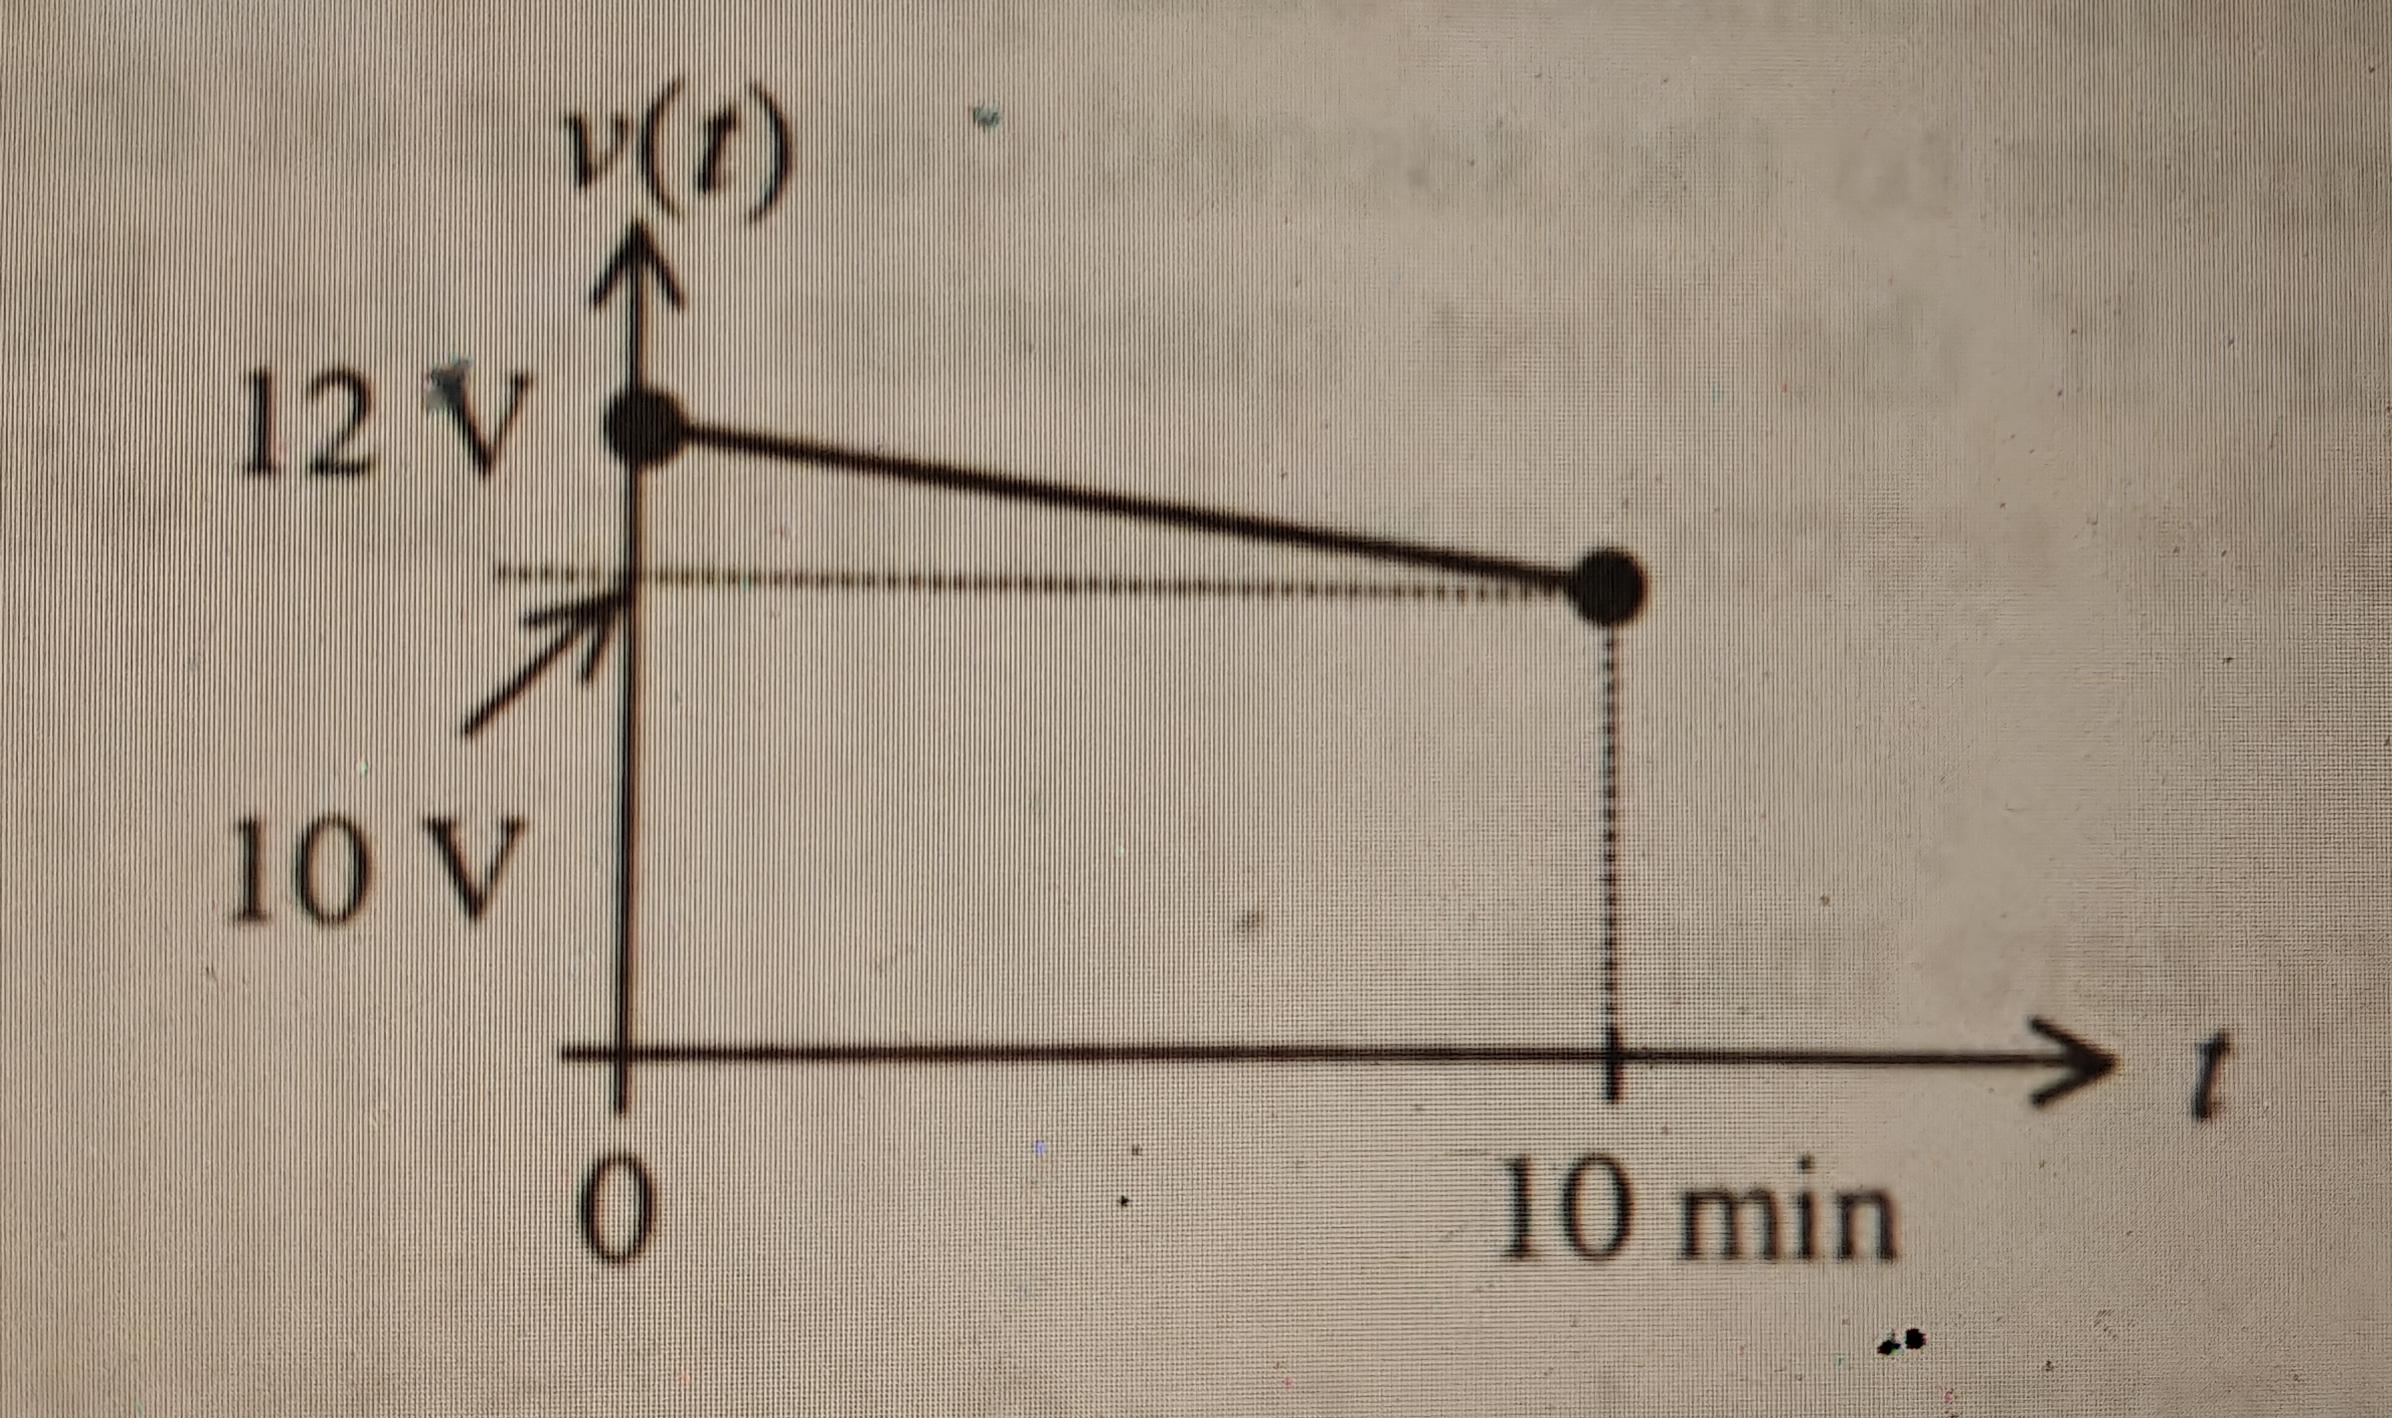
\includegraphics[width=0.5\columnwidth]{figs/fig_1.jpg}
    \caption{\centering v vs t graph}
    \label{fig:placeholder_1}
\end{figure}
\begin{enumerate}
\begin{multicols}{4}
\item 220 J
\item 12 kJ
\item 13.2 kJ
\item 14.4 kJ
\end{multicols}
\end{enumerate}
\hfill $\brak{\text{GATE EC 2009}}$

\item In an \textbf{n}-type silicon crystal at room temperature, which of the following can have a concentration of $4 \text{ x } 10^{19}  cm^{-3}$ ?
\begin{enumerate}
\begin{multicols}{4}
\item Silicon atoms
\item Holes
\item Dopant atoms
\item Valence electrons
\end{multicols}
\end{enumerate}
\hfill $\brak{\text{GATE EC 2009}}$

\item The full form of abbreviations TTL and CMOS in reference to logic families are 
\begin{enumerate}
\item Triple Transistor Logic and Chip Metal Oxide Semiconductor
\item Tristate Transistor Logic and Chip Metal Oxide Semiconductor
\item Transistor Transistor Logic and Complementary Metal Oxide Semiconductor
\item Tristate Transistor Logic and Complementary Metal Oxide Semiconductor
\end{enumerate}
\hfill $\brak{\text{GATE EC 2009}}$

\item The ROC of Z-tranform of the discrete time sequence $x(n)$= $\brak{\frac{1}{3}}^n u\brak{n}$ - $\brak{\frac{1}{3}}^n u\brak{-n-1}$ is 
\begin{enumerate}
\item $\frac{1}{3} <|z| <\frac{1}{2}$
\item $|z| >\frac{1}{2}$
\item $|z| <\frac{1}{3}$
\item $2<|z|<3$
\end{enumerate}
\hfill $\brak{\text{GATE EC 2009}}$

\item The magnitude plot of a rational transfer function $G\brak{s}$ with real coefficients is shown below in the $\figref{fig:placeholder_2}$. Which of the following compensator has such a magnitude plot ?
\begin{figure}[H]
    \centering
    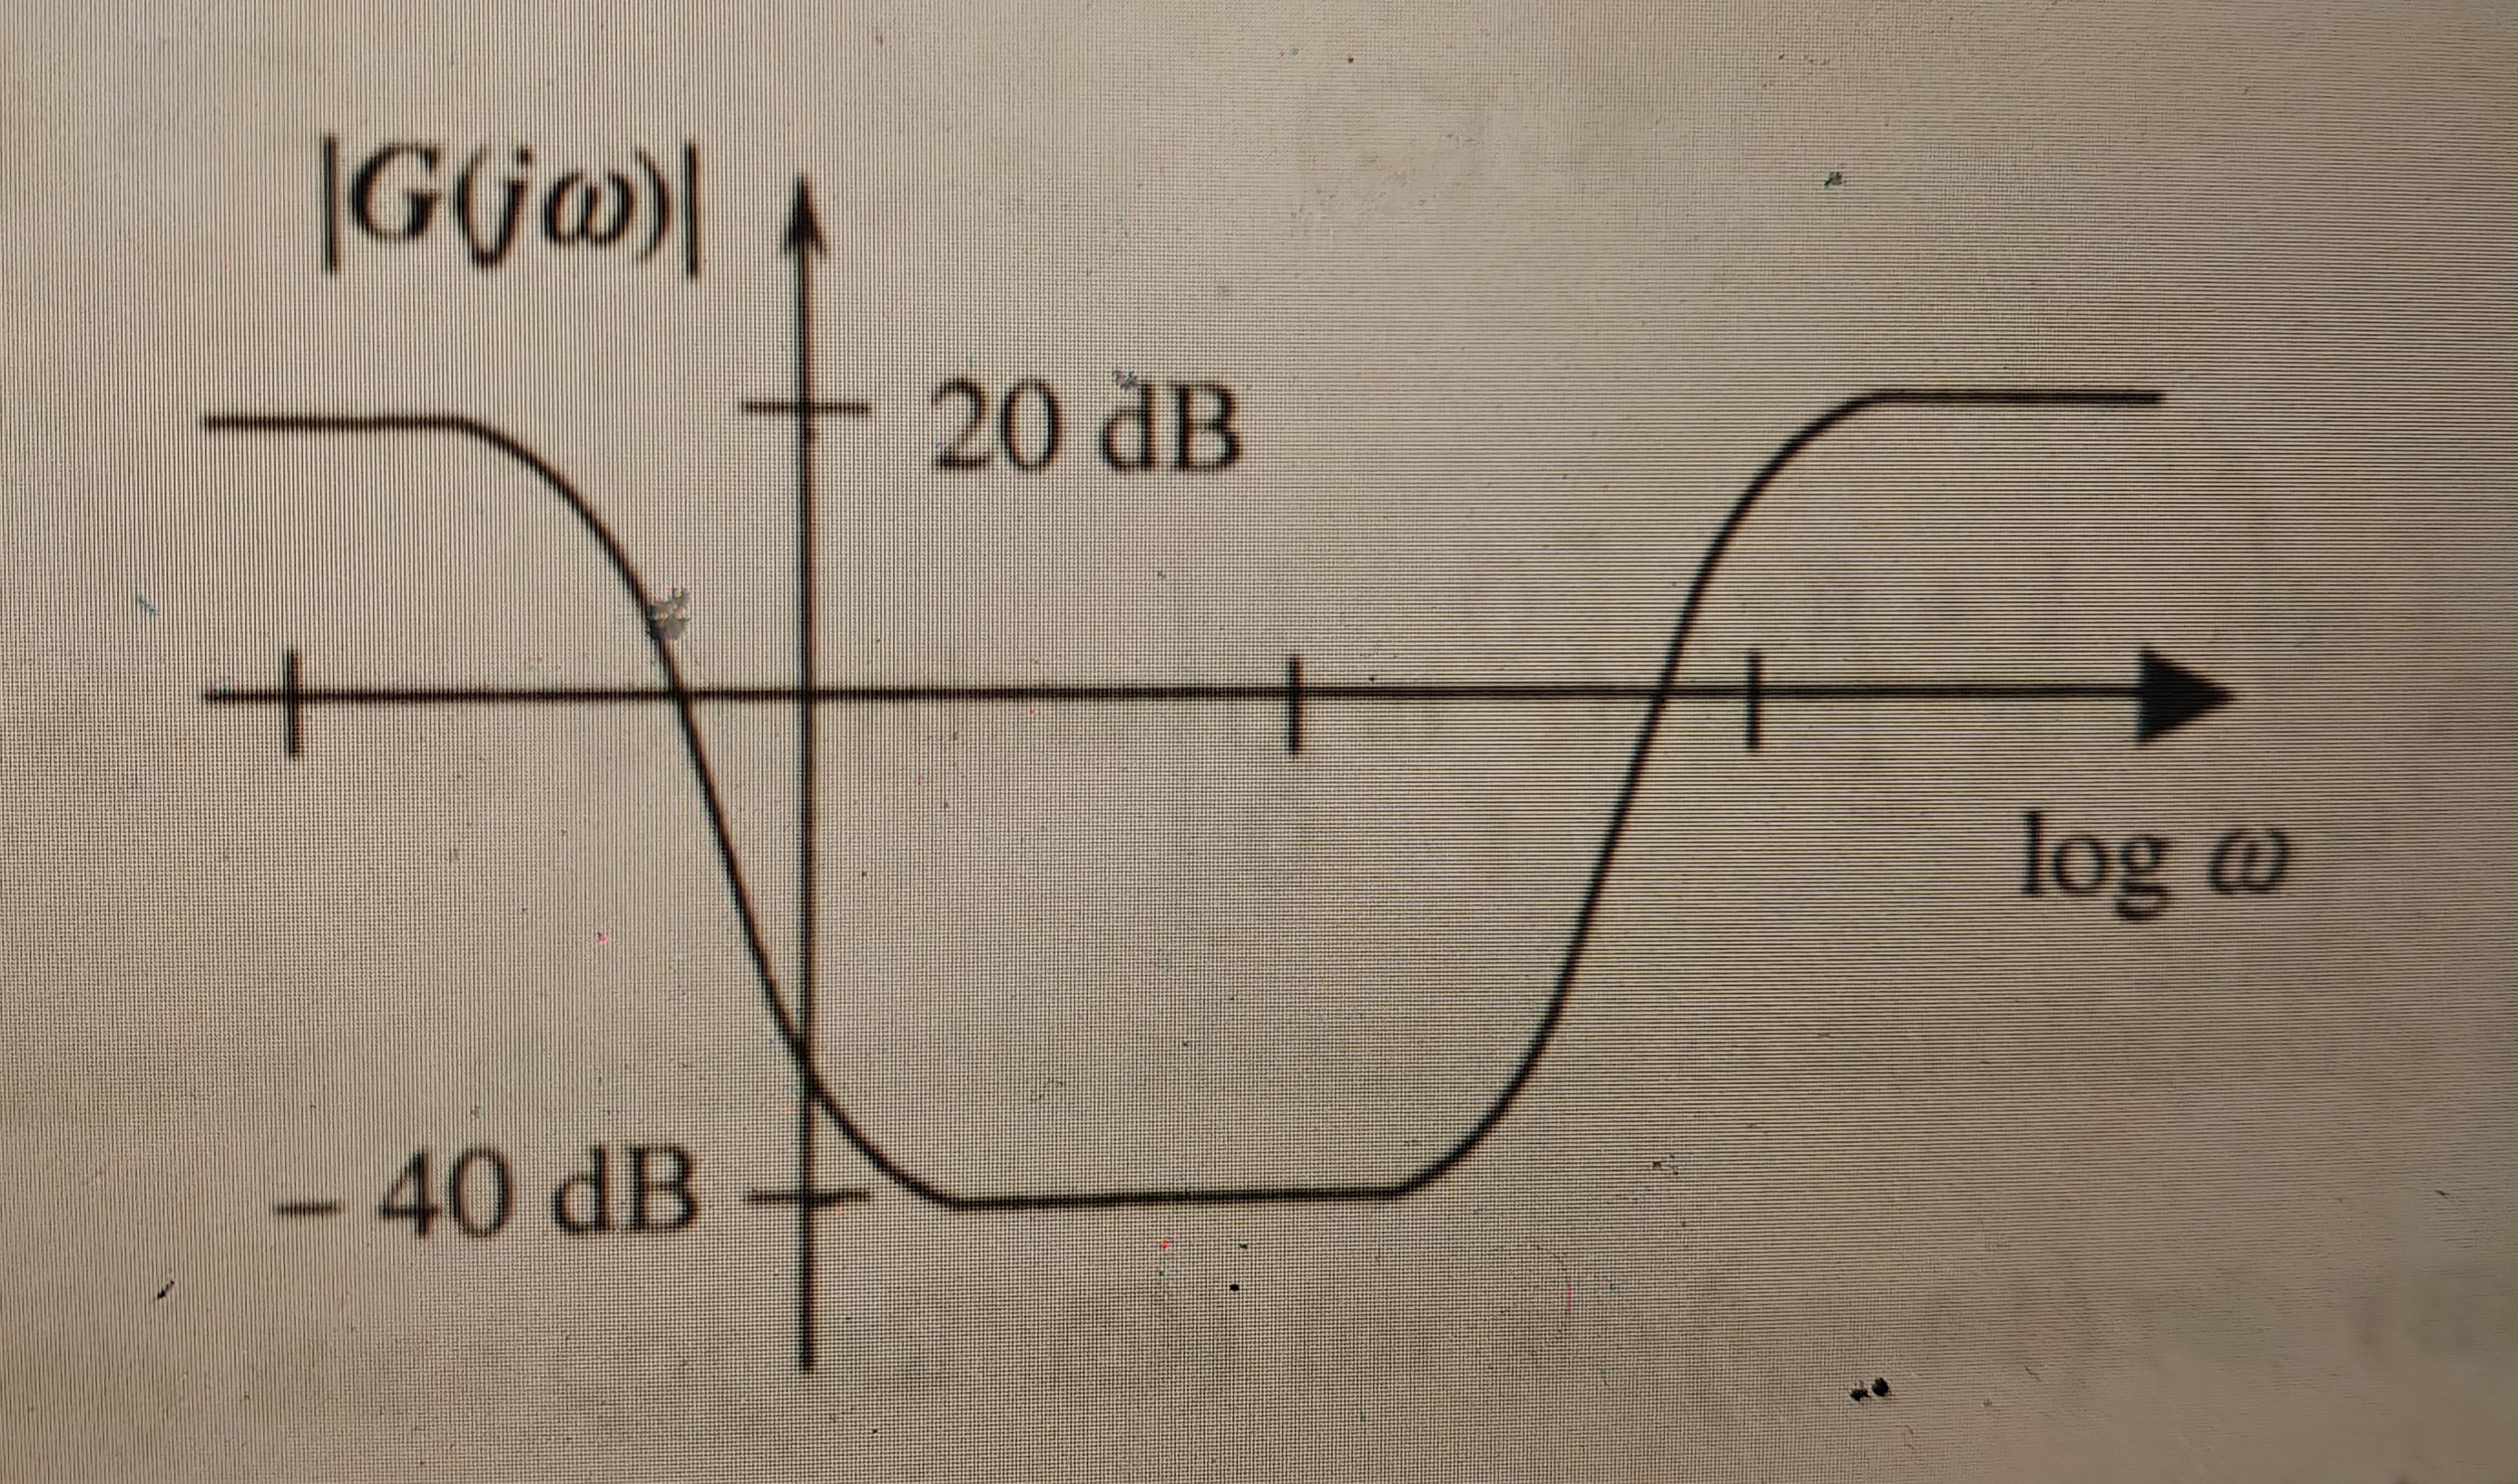
\includegraphics[width=0.5\columnwidth]{figs/fig_2.jpg}
    \caption{\centering Magnitude plot of function $G\brak{s}$ }
    \label{fig:placeholder_2}
\end{figure}
\begin{enumerate}
\begin{multicols}{2}
\item Lead compensator
\item Lag compensator
\item PID compensator
\item Lead-lag compensator
\end{multicols}
\end{enumerate}
\hfill $\brak{\text{GATE EC 2009}}$

\item A white noise process $X\brak{t}$ with two-sided power spectral density $1$ x $10^{-10} W/Hz$ is input into a filter whose magnitude squared response is shown below in the $\figref{fig:placeholder_3}$.
\begin{figure}[H]
    \centering
    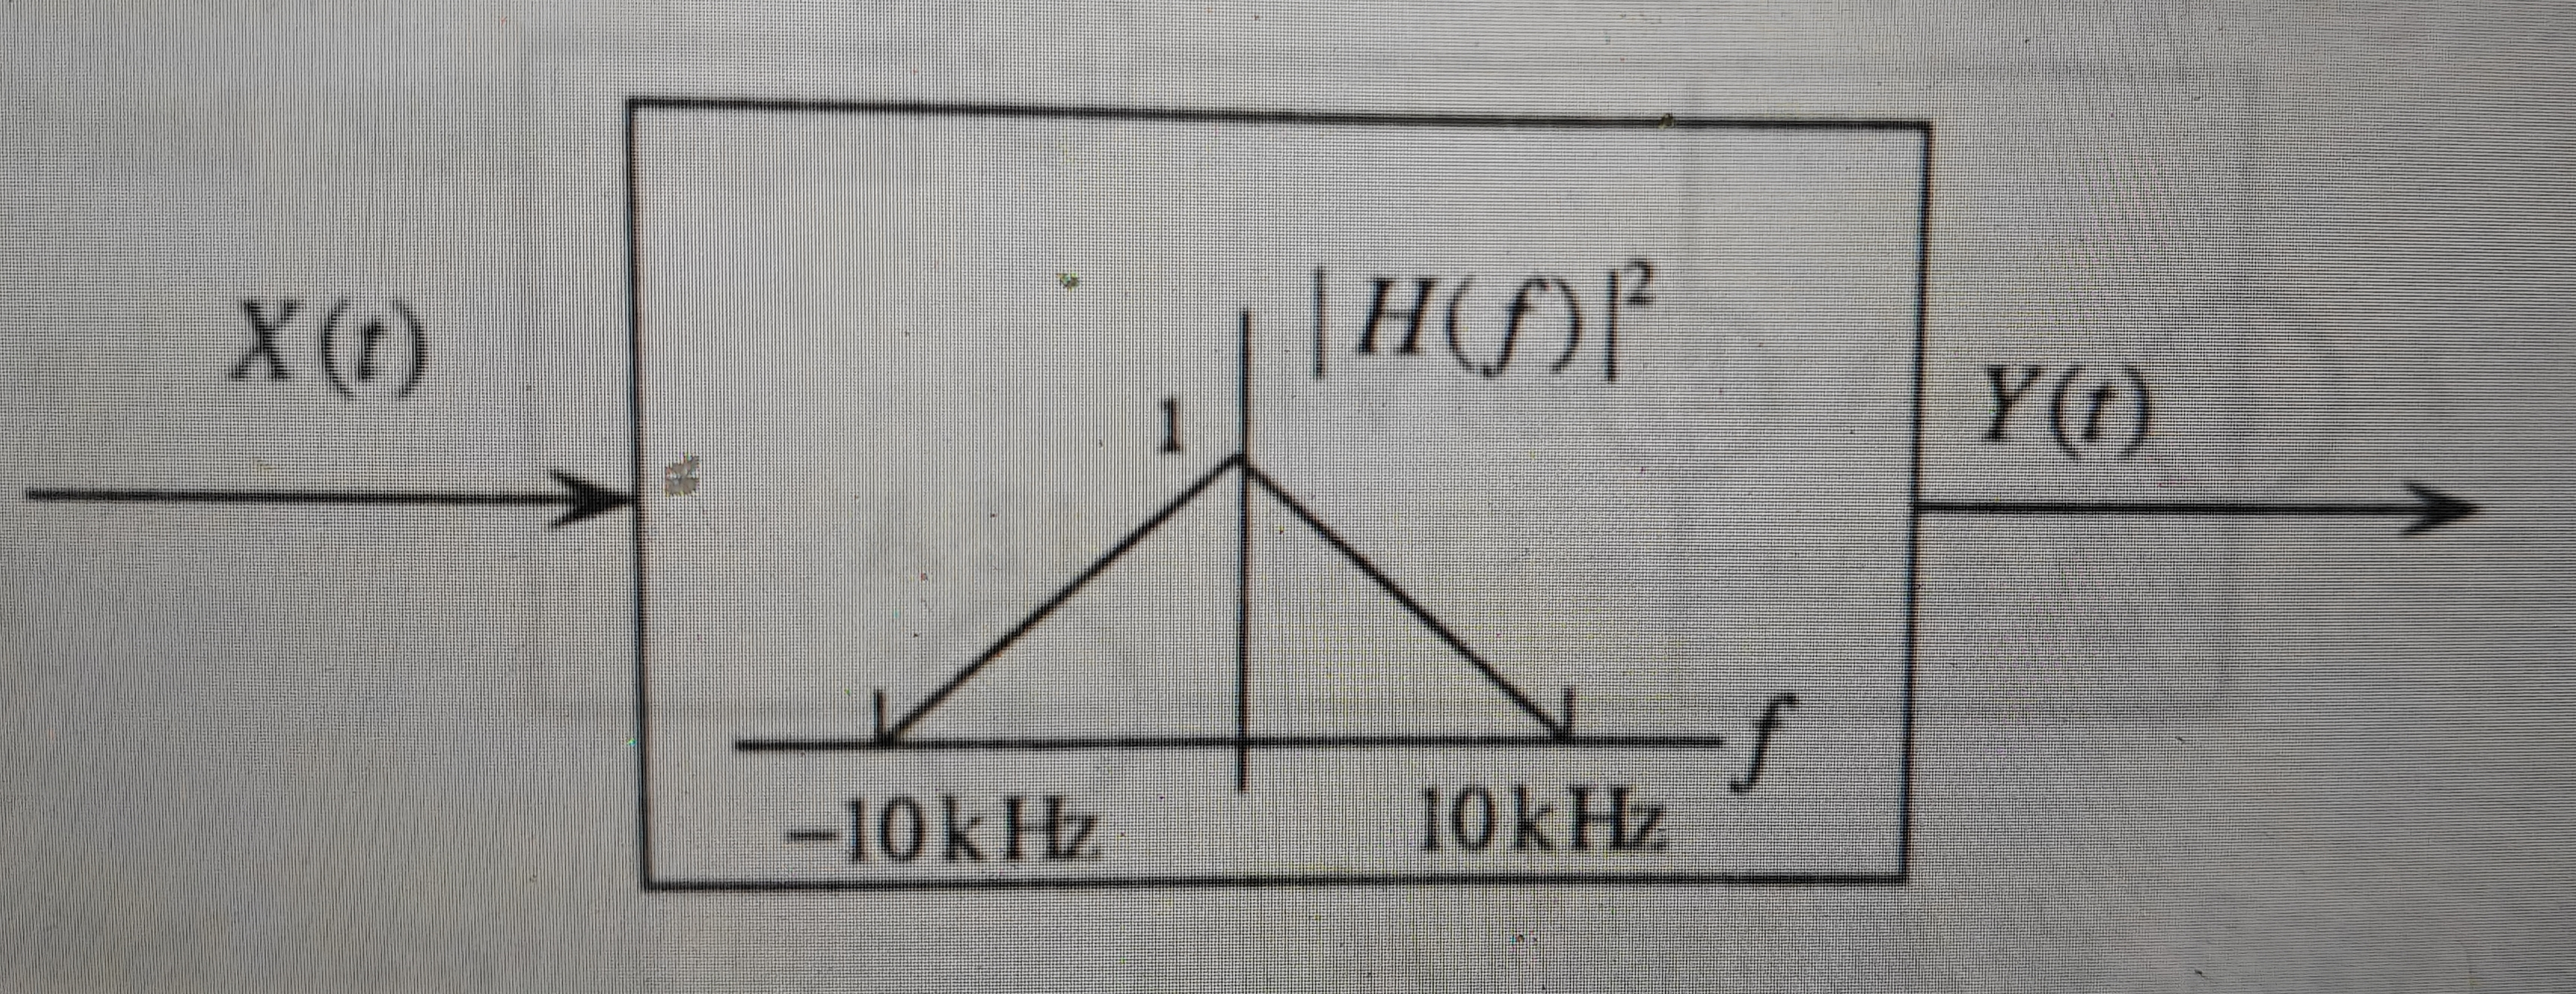
\includegraphics[width=0.5\columnwidth]{figs/fig_3.jpg}
    \caption{\centering for Q-9}
    \label{fig:placeholder_3}
\end{figure}
The power output process $Y\brak{t}$ is given by 
\begin{enumerate}
\begin{multicols}{4}
\item 1
\item 2
\item 3
\item 4
\end{multicols}
\end{enumerate}
\hfill $\brak{\text{GATE EC 2009}}$

\item Which of the following statements is true regarding the fundamental node of the metallic waveguides shown in the $\figref{fig:placeholder_4}$?
\begin{figure}[H]
    \centering
    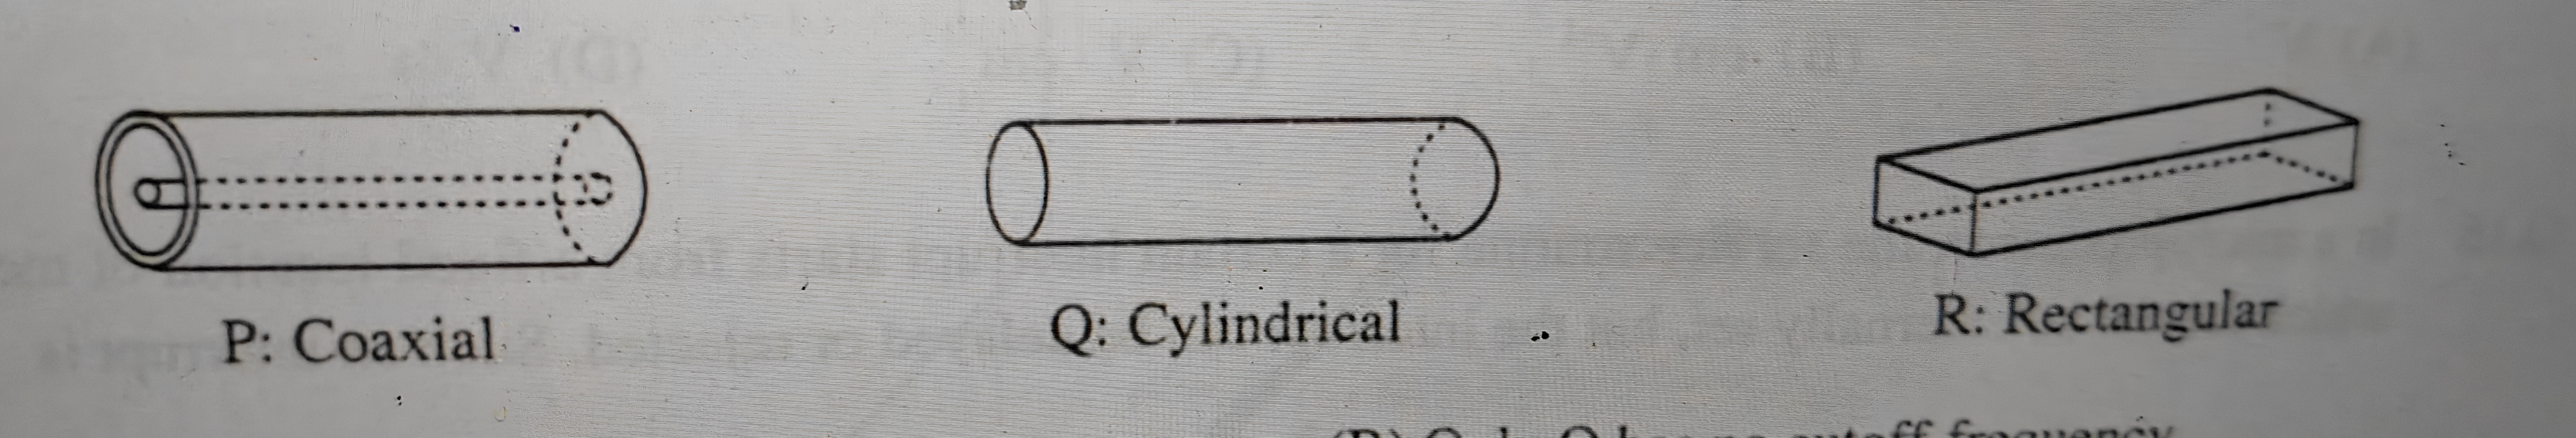
\includegraphics[width=0.5\columnwidth]{figs/fig_4.jpg}
    \caption{\centering for Q-10}
    \label{fig:placeholder_4}
\end{figure}
\begin{enumerate}
\begin{multicols}{2}
\item Only P has no cutoff-frequency
\item Only Q has no cutoff-frequency
\item Only R has no cutoff-frequency
\item All three have cutoff-frequencies
\end{multicols}
\end{enumerate}
\hfill $\brak{\text{GATE EC 2009}}$

\item A fair coin is tossed $10$ times. What is the probability that ONLY the first two will yield heads?
\begin{enumerate}
\begin{multicols}{4}
\item $\brak{\frac{1}{2}}^{2}$
\item $^{10}C_2 \brak{\frac{1}{2}}^{2}$
\item $\brak{\frac{1}{2}}^{10}$
\item $^{10}C_2 \brak{\frac{1}{2}}^{10}$
\end{multicols}
\end{enumerate}
\hfill $\brak{\text{GATE EC 2009}}$

\item If the power spectral density of stationary random process is a sine-squared function of frequency as shown in $\figref{fig:placeholder_5}$, the shape of its autocorrelation is
\begin{figure}[H]
    \centering
    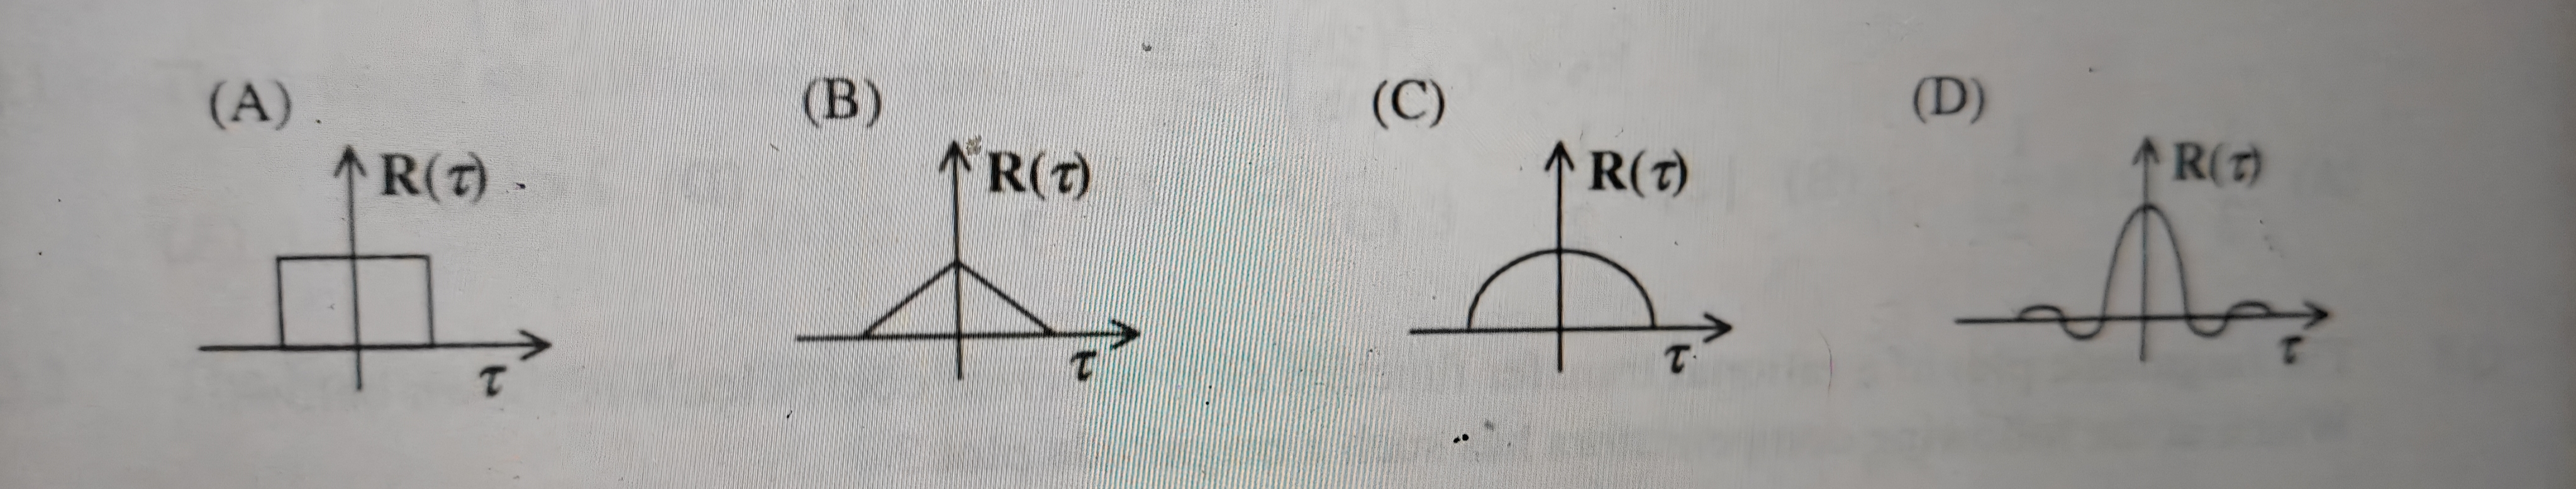
\includegraphics[width=0.5\columnwidth]{figs/fig_5.jpg}
    \caption{\centering for Q-12}
    \label{fig:placeholder_5}
\end{figure}
\hfill $\brak{\text{GATE EC 2009}}$

\item If $f\brak{z} = c_0 + c_1z^{-1}$, then $\oint_{unit circle} \frac{1+f(z)}{z} dz$ is given by
\begin{enumerate}
\begin{multicols}{4}
\item $2\pi c_1$
\item $2\pi \brak{1+c_0}$
\item $2\pi jc_1$
\item $2\pi j\brak{1+c_0}$
\end{multicols}
\end{enumerate}
\hfill $\brak{\text{GATE EC 2009}}$

\item In the interconnection of ideal sources shown in $\figref{fig:placeholder_6}$, it is known that the $60 V$ source is absorbing power.
\begin{figure}[H]
    \centering
    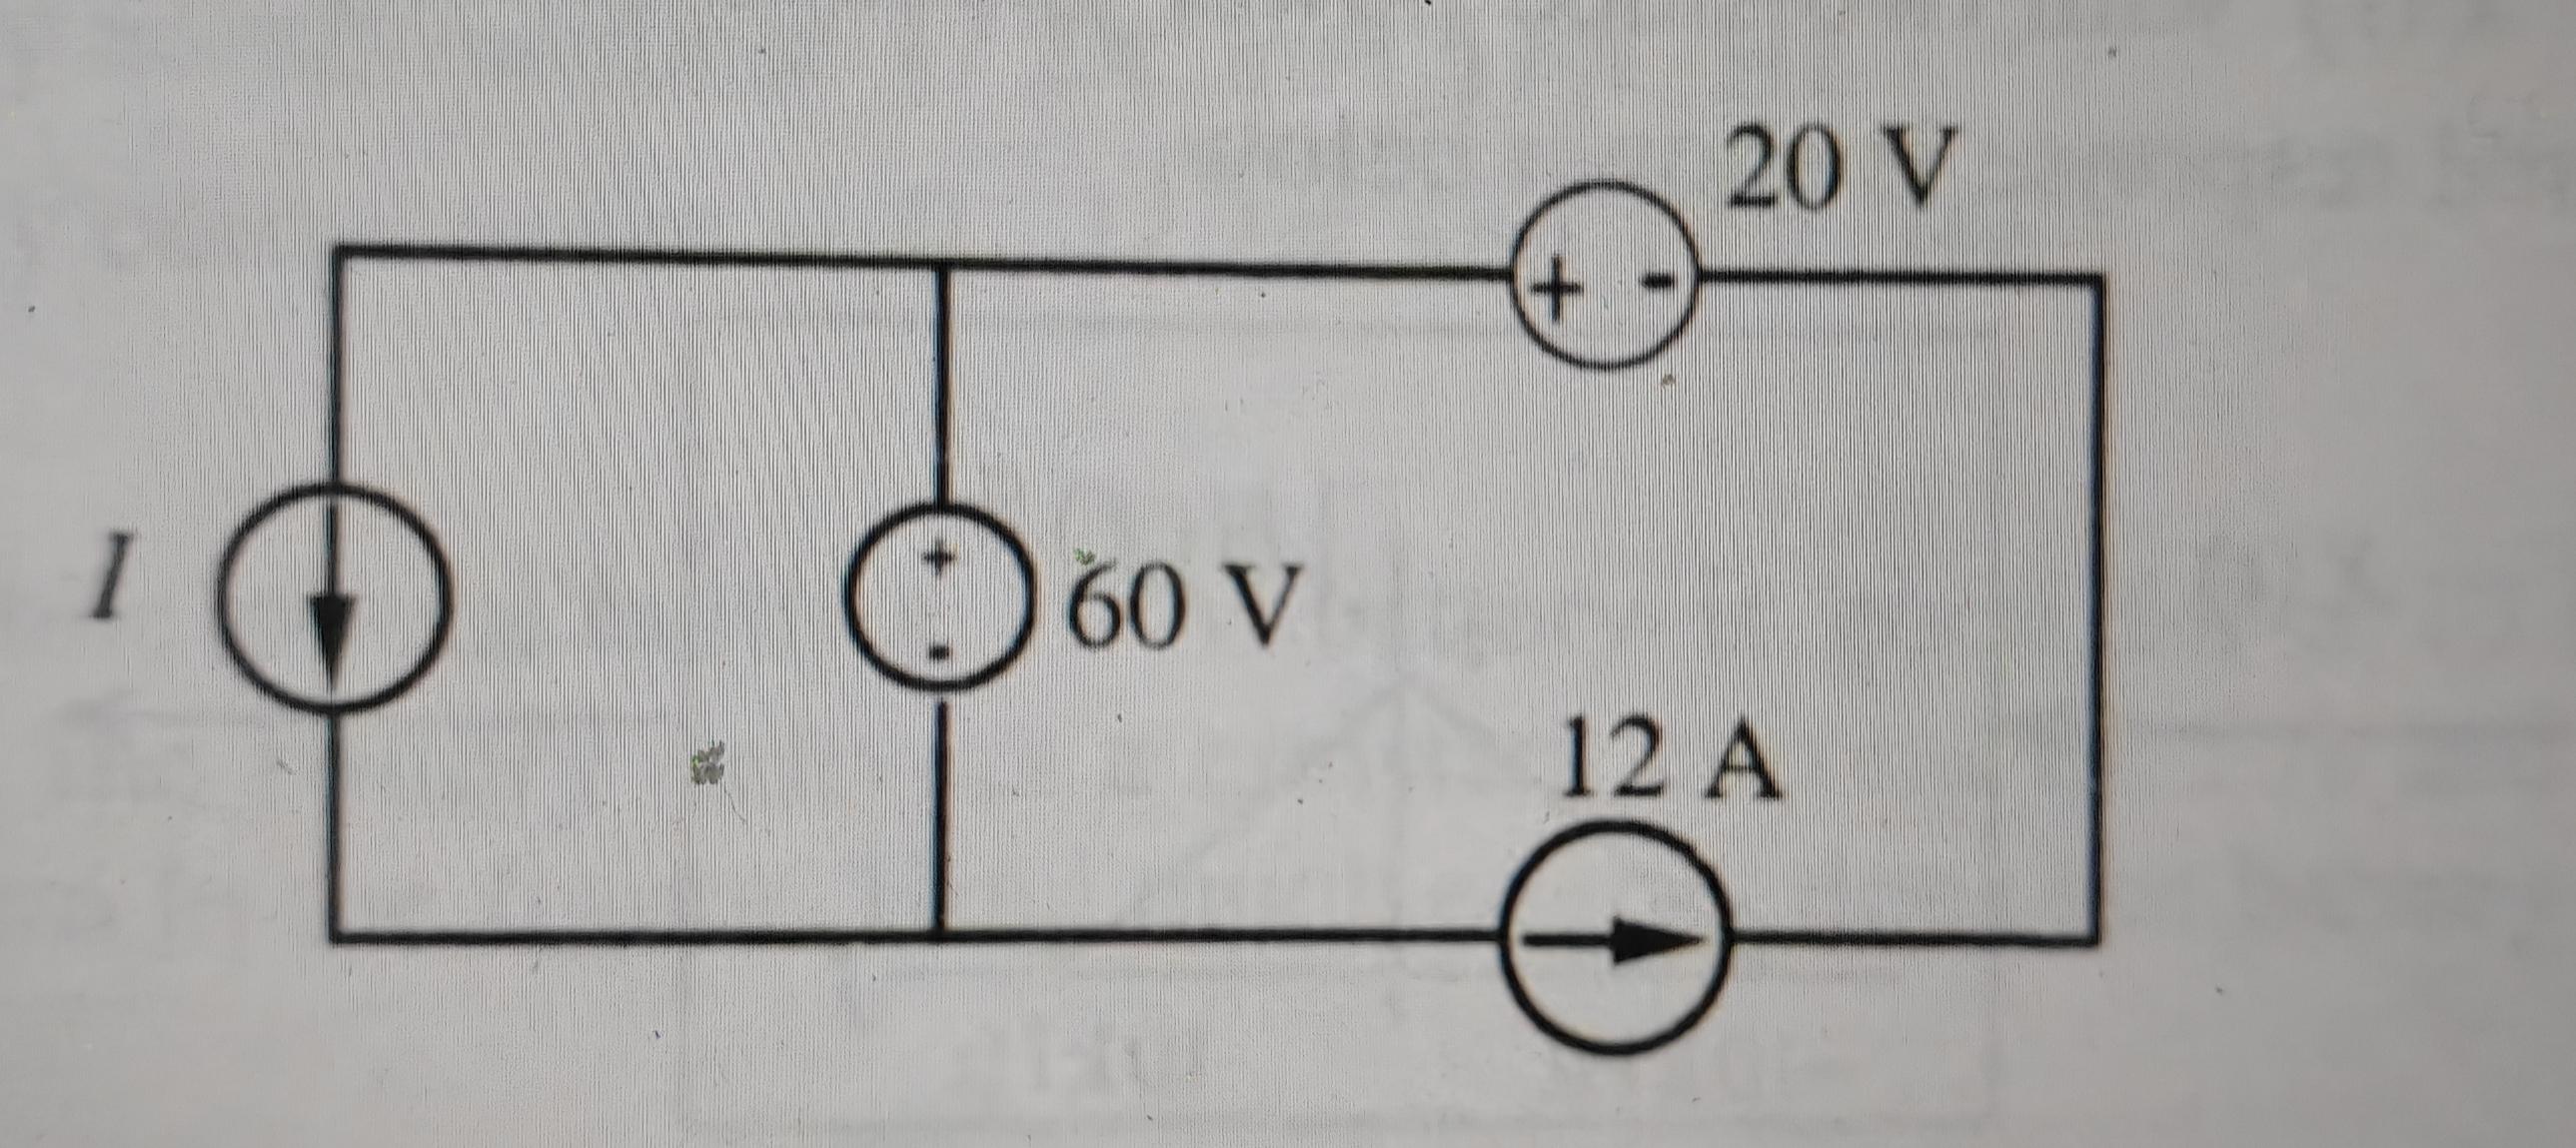
\includegraphics[width=0.5\columnwidth]{figs/fig_6.jpg}
    \caption{\centering Circuit for Q-14}
    \label{fig:placeholder_6}
\end{figure}
Which of the following can the value of current source ${I}$ ?

\begin{enumerate}
\begin{multicols}{4}
\item 10 $A$
\item 13 $A$
\item 15 $A$
\item 18 $A$
\end{multicols}
\end{enumerate}
\hfill $\brak{\text{GATE EC 2009}}$

\item The ratio of the mobility to the diffusion coefficient in a semiconductor has the units 
\begin{enumerate}
\begin{multicols}{4}
\item $V^{-1}$
\item $cm . V^{-1}$
\item $V . cm^{-1}$
\item $V . s$
\end{multicols}
\end{enumerate}
\hfill $\brak{\text{GATE EC 2009}}$

\item In a microprocessor, the service routine for a certain interrupt starts from a fixed location of a memory which cannot be externally set, but the interrupt can be delayed or rejected. Such an interrupt is
\begin{enumerate}
\item non-maskable and non-vectored 
\item maskable and non-vectored 
\item non-maskable and vectored
\item maskable and vectored
\end{enumerate}
\hfill $\brak{\text{GATE EC 2009}}$

\item If the transfer function of the following network is $\frac{V_o\brak{s}}{V_t\brak{s}} = \frac{1}{2+ sCR}$, the value of load resistance $R_L$ is
\begin{figure}[H]
    \centering
    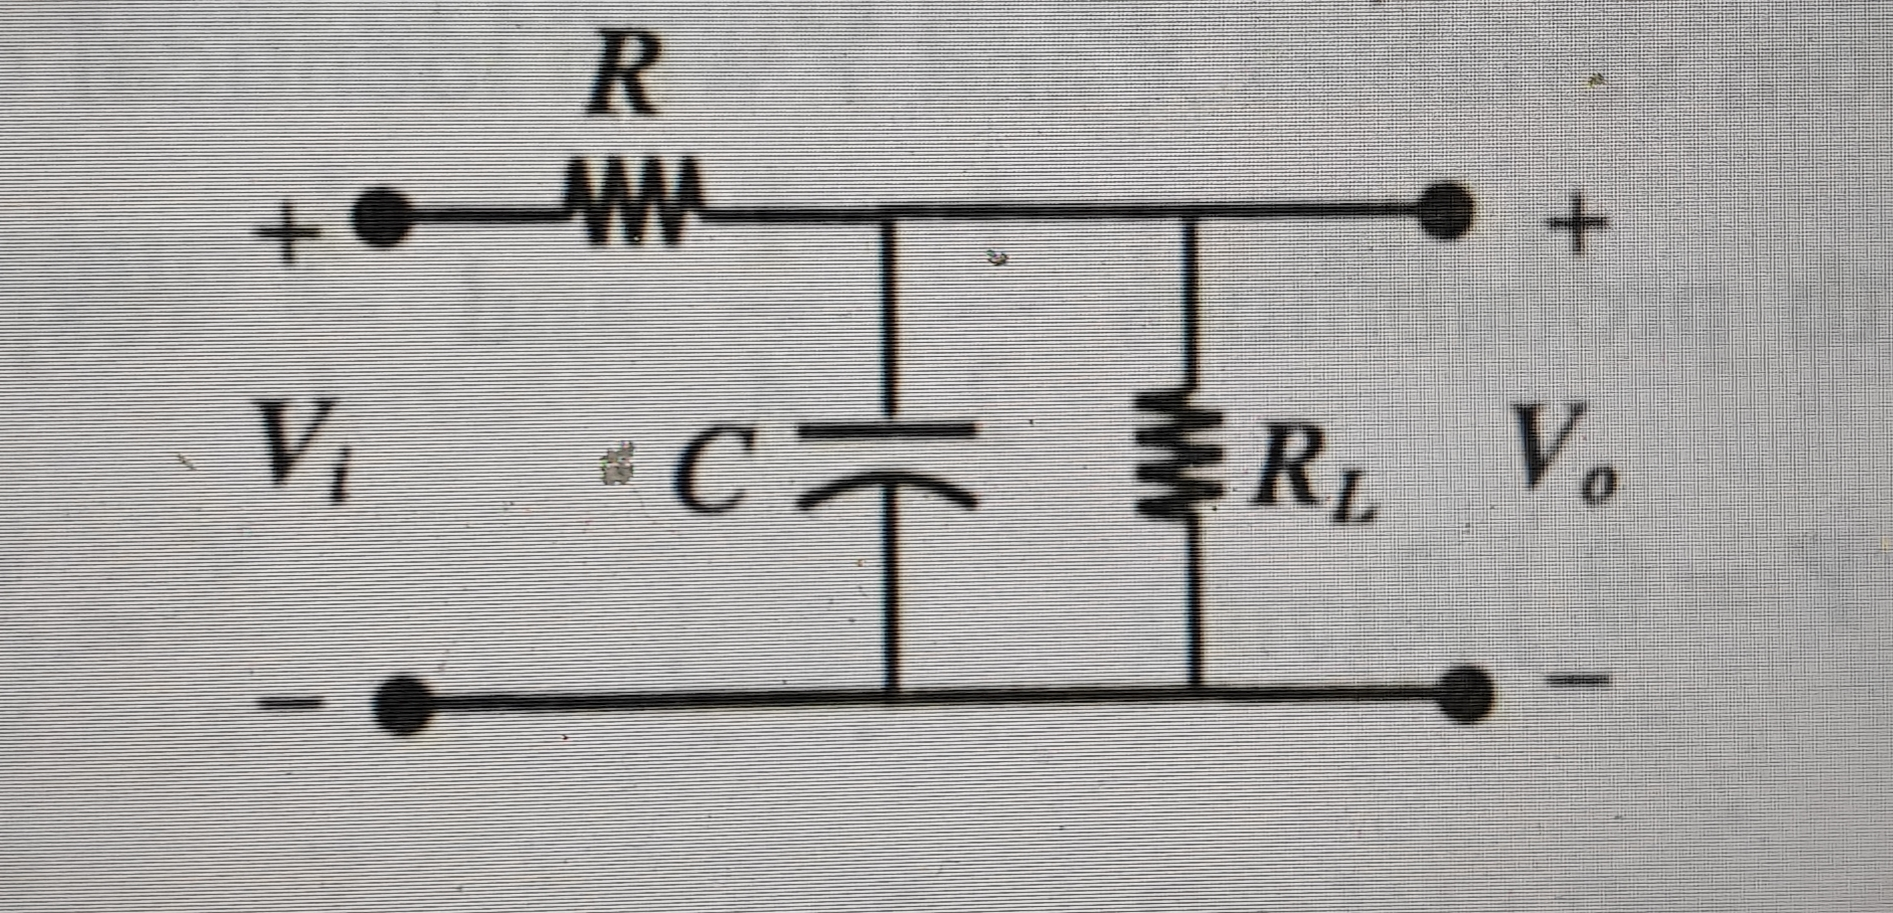
\includegraphics[width=0.5\columnwidth]{figs/fig_7.jpg}
    \caption{\centering Network for Q-17}
    \label{fig:placeholder_7}
\end{figure}
\begin{enumerate}
\begin{multicols}{4}
\item $R/4$
\item $R/2$
\item $R$
\item $2R$
\end{multicols}
\end{enumerate}
\hfill $\brak{\text{GATE EC 2009}}$

\item Consider the system $\frac{dx}{dt} = Ax +Bu$ with $A= \myvec{1&&0 \\ 0 && 1}$
 and B= 
$\myvec{p\\q}$ where p and q are arbitrary real numbers. Which of the following statements is true about the contrallability of the system is true?
\begin{enumerate}
\item The system is completely state controllable for any non zero values of $p$ and $q$
\item Only $p=0$ and $q=0$ result in controllability
\item The system is uncontrollable for any values of $p$ and $q$
\item We cannot conclude about controllability from the given data
\end{enumerate}
\hfill $\brak{\text{GATE EC 2009}}$

\item For a message signal $m\brak{t} = \cos {\brak{2\pi f_m t}}$ and the carrier of the frequency ${f_c}$, which of the following represent a single side band $\brak{SSB}$ signal?
\begin{enumerate}
\begin{multicols}{2}
    \item $\cos\brak{2\pi f_m t} \cos\brak{2\pi f_c t}$
    \item $\cos\brak{2\pi f_c t}$
    \item $\cos\sbrak{2\pi \brak{f_c + f_m} t}$
    \item $\sbrak{1+\cos\brak{2\pi f_m t}} \cos\brak{2\pi f_c t}$
\end{multicols}
\end{enumerate}

\item Two infinitely long wires carrying current are as shown in the $\figref{fig:placeholder_8}$ below. One wire is in $y-z$ plane and parallel to the $y$-axis. The other wire is in the $x-y$ plane and parallel to the $x$-axis. Which components of the resulting magnetic fields are non-zero at origin?
\begin{figure}[H]
    \centering
    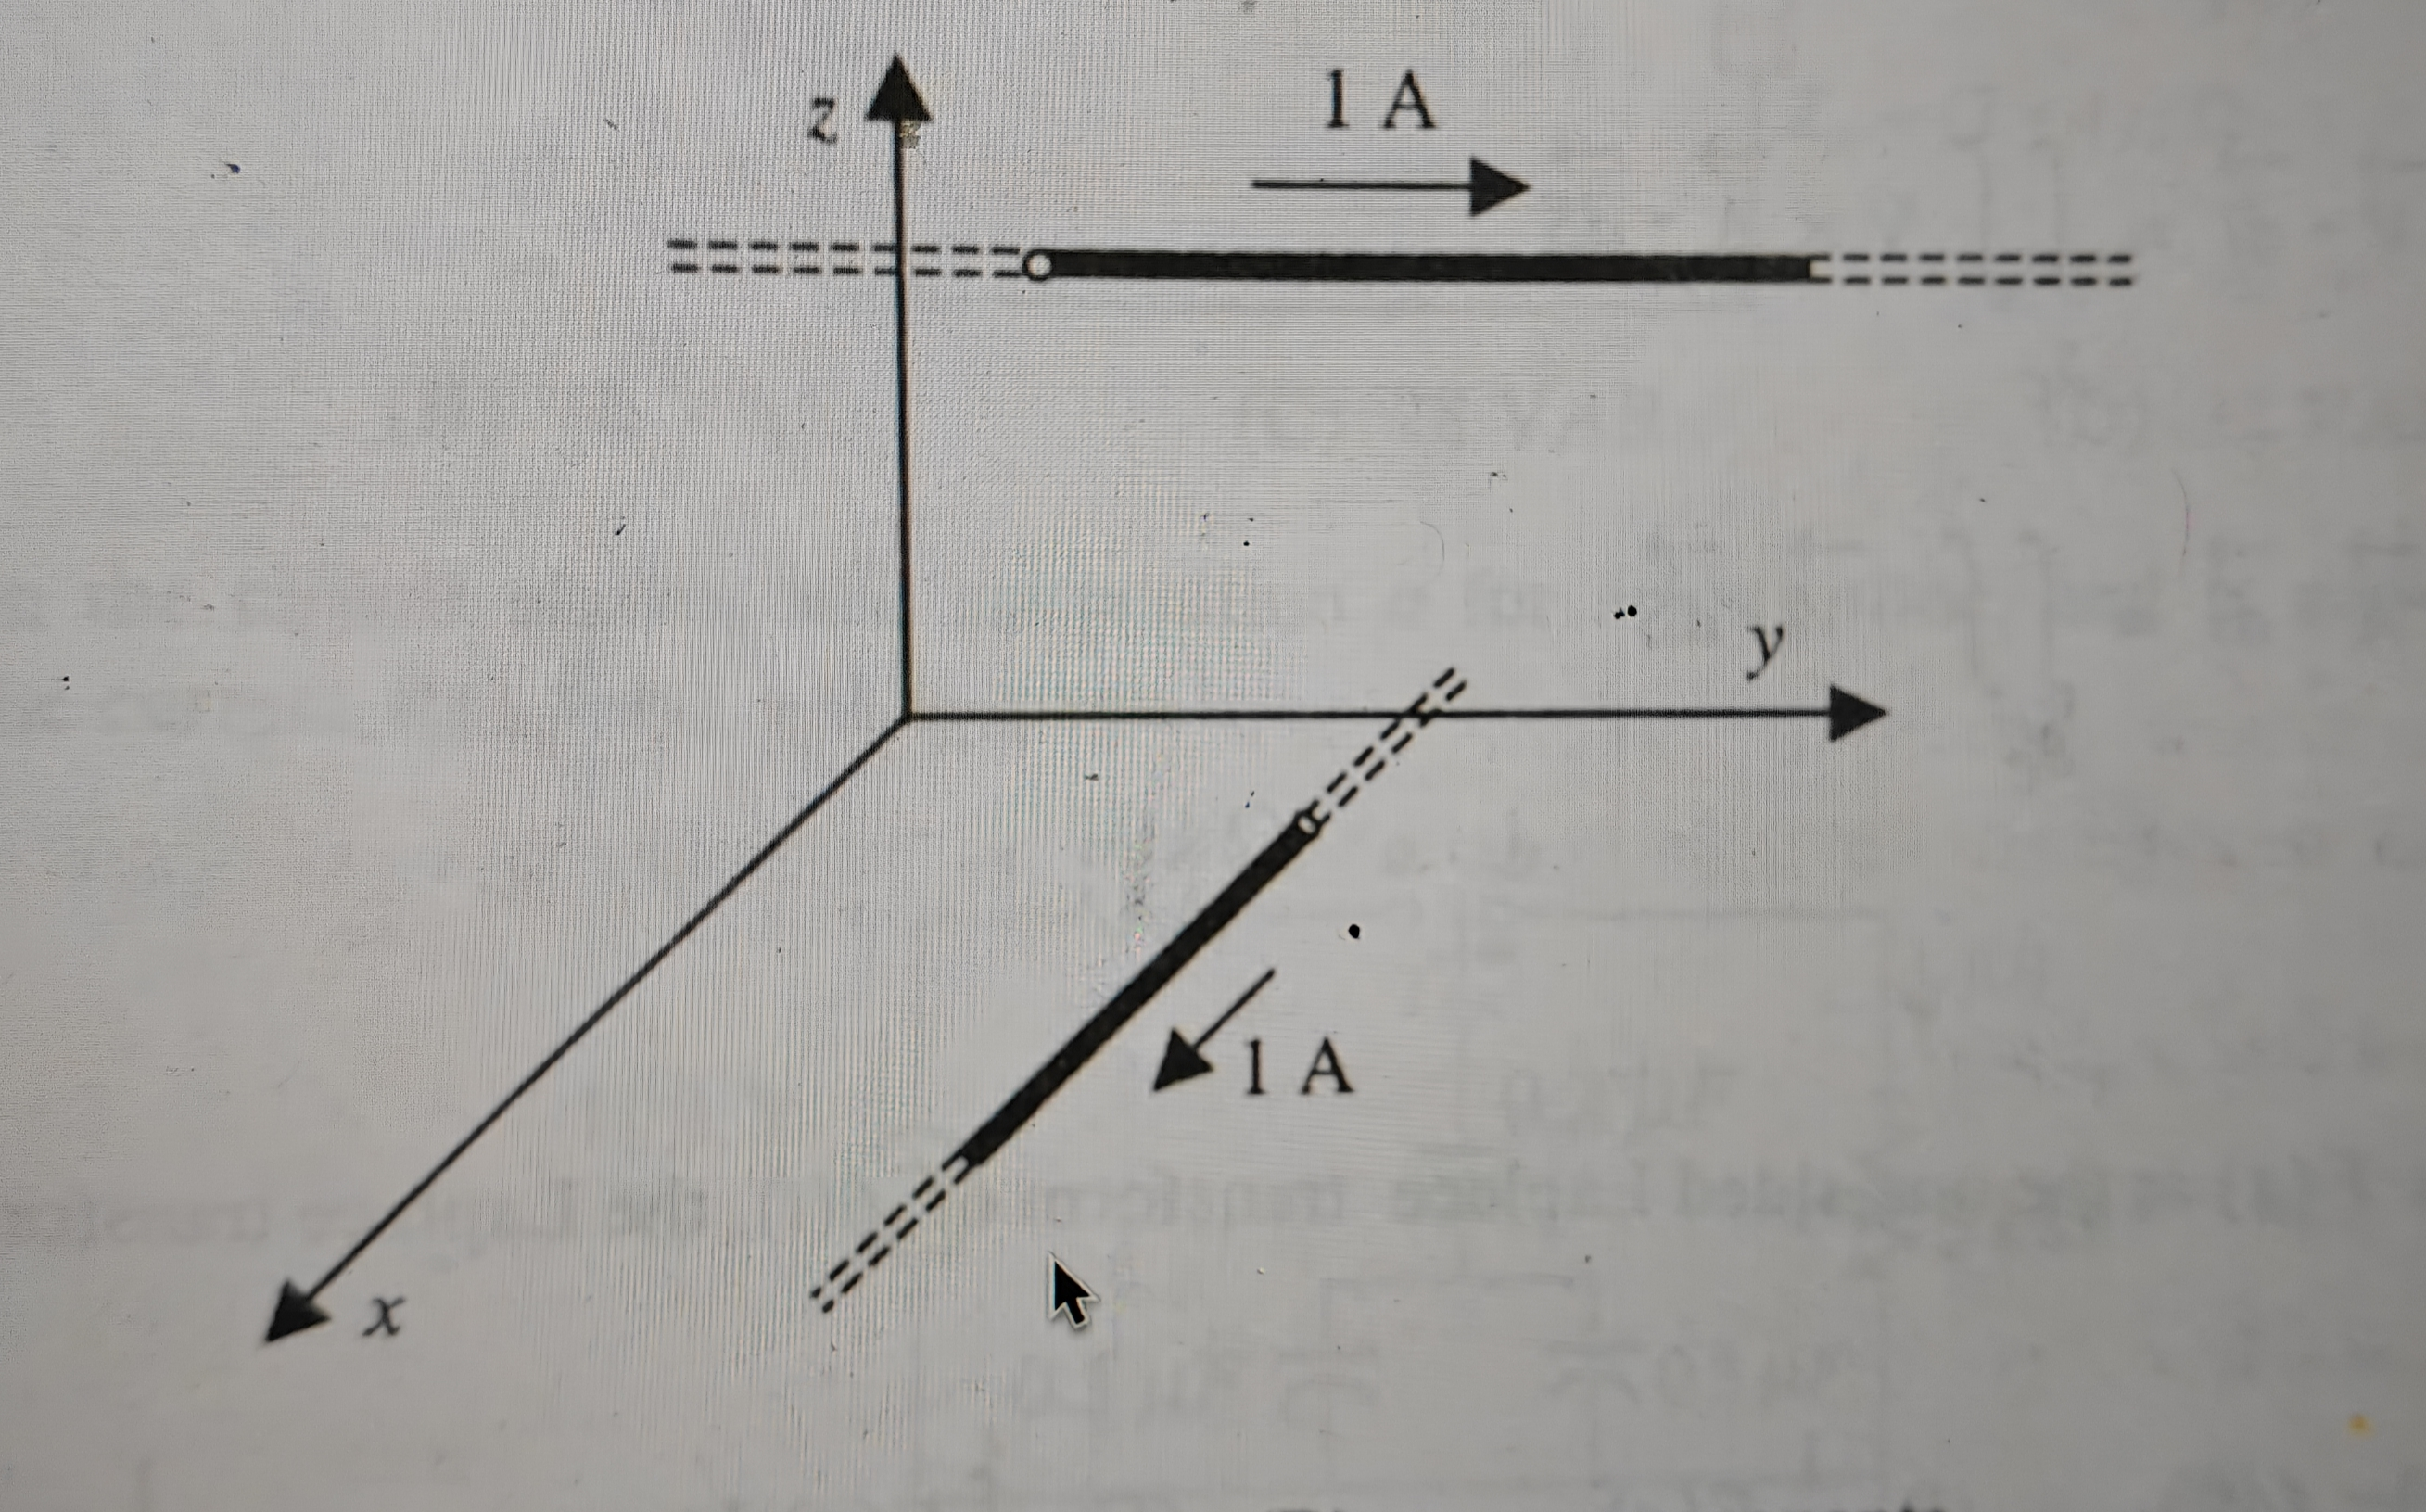
\includegraphics[width=0.5\columnwidth]{figs/fig_8.jpg}
    \caption{\centering For Q-20}
    \label{fig:placeholder_8}
\end{figure}
\begin{enumerate}
\begin{multicols}{2}
    \item $x,y,z$ components
    \item $x,y$ components
    \item $y,z$ components
    \item $x,z$ components
\end{multicols}
\end{enumerate}
\hfill $\brak{\text{GATE EC 2009}}$
\item Consider two independent random variables $X$ and $Y$ with identical distributions. The variables $X$ and $Y$ take values 0, 1 and 2 with probabilities $\frac{1}{2}, \frac{1}{4} and  \quad \frac{1}{4}$ respectively. What is the conditional probability $P\brak{X+Y=2 \quad| \quad X-Y=0}$ ?

\begin{enumerate}
\begin{multicols}{4}
\item 0
\item $\frac{1}{16}$
\item $\frac{1}{6}$
\item 1
\end{multicols}
\end{enumerate}
\hfill $\brak{\text{GATE EC 2009}}$

\item The Taylor series expansion of $\frac{\sin x}{x-\pi}$ at x=$\pi$ is given by
\begin{enumerate}
\begin{multicols}{2}
\item 1+ $\frac{\brak{x-\pi}^2}{3!}$ + ..
\item -1-$\frac{\brak{x-\pi}^2}{3!}$ + ..
\item 1-$\frac{\brak{x-\pi}^2}{3!}$ + ..
\item -1+ $\frac{\brak{x-\pi}^2}{3!}$ + ..
\end{multicols}
\end{enumerate}
\hfill $\brak{\text{GATE EC 2009}}$

\item If a vector field $\Vec{V}$ is related to another vector field $\Vec{A}$ through $\Vec{V}=\nabla$ x $\Vec{A}$ , which of the following is true? Note: $C$ and $S_c$ refer to any closed contour and any surface whose boundary is $C$.
\begin{enumerate}
    \item $\oint_c \Vec{V}\cdot \Vec{dl}$ = $\int_{S_c} \int \Vec{A}\cdot \Vec{dS}$
    \item $\oint_c \Vec{A}\cdot \Vec{dl}$ = $\int_{S_c} \int \Vec{V}\cdot \Vec{dS}$
    \item $\oint_c  \nabla$ x $\Vec{V}\cdot \Vec{dl}$ = $\int_{S_c} \int \nabla$ x $\Vec{A}\cdot \Vec{dS}$
    \item $\oint_c \nabla$ x $\Vec{A}\cdot \Vec{dl}$ = $\int_{S_c} \int \Vec{V}\cdot \Vec{dS}$
\end{enumerate}
\hfill $\brak{\text{GATE EC 2009}}$

\item Given that $F\brak{s})$ is the one-sided Laplace transform of $f\brak{t})$, the Laplace transform of $\int_0^t f\brak{\tau} d\tau$ is 
\begin{enumerate}
\begin{multicols}{2}
\item $sF\brak{s}-f\brak{0}$
\item $\frac{1}{s} F\brak{s}$
\item $\int_0^t F\brak{\tau} d\tau$
\item $\frac{1}{s}\sbrak{F\brak{s}-f\brak{0}}$
\end{multicols}
\end{enumerate}
\hfill $\brak{\text{GATE EC 2009}}$

\item Match each differential equation in Group I to its family of solution curves from Group II.
\begin{align*}
    \begin{tabular}{ll}
\textbf{Group I} & \textbf{Group II} \\
P. $\frac{dy}{dx}=\frac{y}{x}$ & 1. Circles \\
Q. $\frac{dy}{dx}=-\frac{y}{x}$ & 2. Straight lines \\
R. $\frac{dy}{dx}=\frac{x}{y}$ & 3. Hyperbolas \\
S. $\frac{dy}{dx}=-\frac{x}{y}$ & \\
\end{tabular}
\end{align*}

\begin{enumerate}
\begin{multicols}{4}
\item P-2,Q-3,R-3,S-1
\item P-1,Q-3,R-2,S-1
\item P-2,Q-1,R-3,S-3
\item P-3,Q-2,R-1,S-2
\end{multicols}
\end{enumerate}
\hfill $\brak{\text{GATE EC 2009}}$

\item The eigen values of the following matrix are 
$\myvec{-1&&3&&5 \\ -3&&-1&&6 \\ 0 && 0 && 3}$
\begin{enumerate}
\begin{multicols}{2}
\item $\text{3,3+5j,6-j}$
\item $\text{-6+5j,3+j, 3-j}$
\item $\text{3+j, 3-j, 5+j}$
\item $\text{3, -1+3j, -1-3j}$
\end{multicols}
\end{enumerate}
\hfill $\brak{\text{GATE EC 2009}}$

\item An AC source of RMS voltage with internal impedance $Z_s = \brak{1+2j} \ohm$ feeds a load of impedance $Z_l = \brak{7+4j} \ohm$ in the $\figref{fig:placeholder_9}$ below. The reactive power consumed by the load is 
\begin{figure}[H]
    \centering
    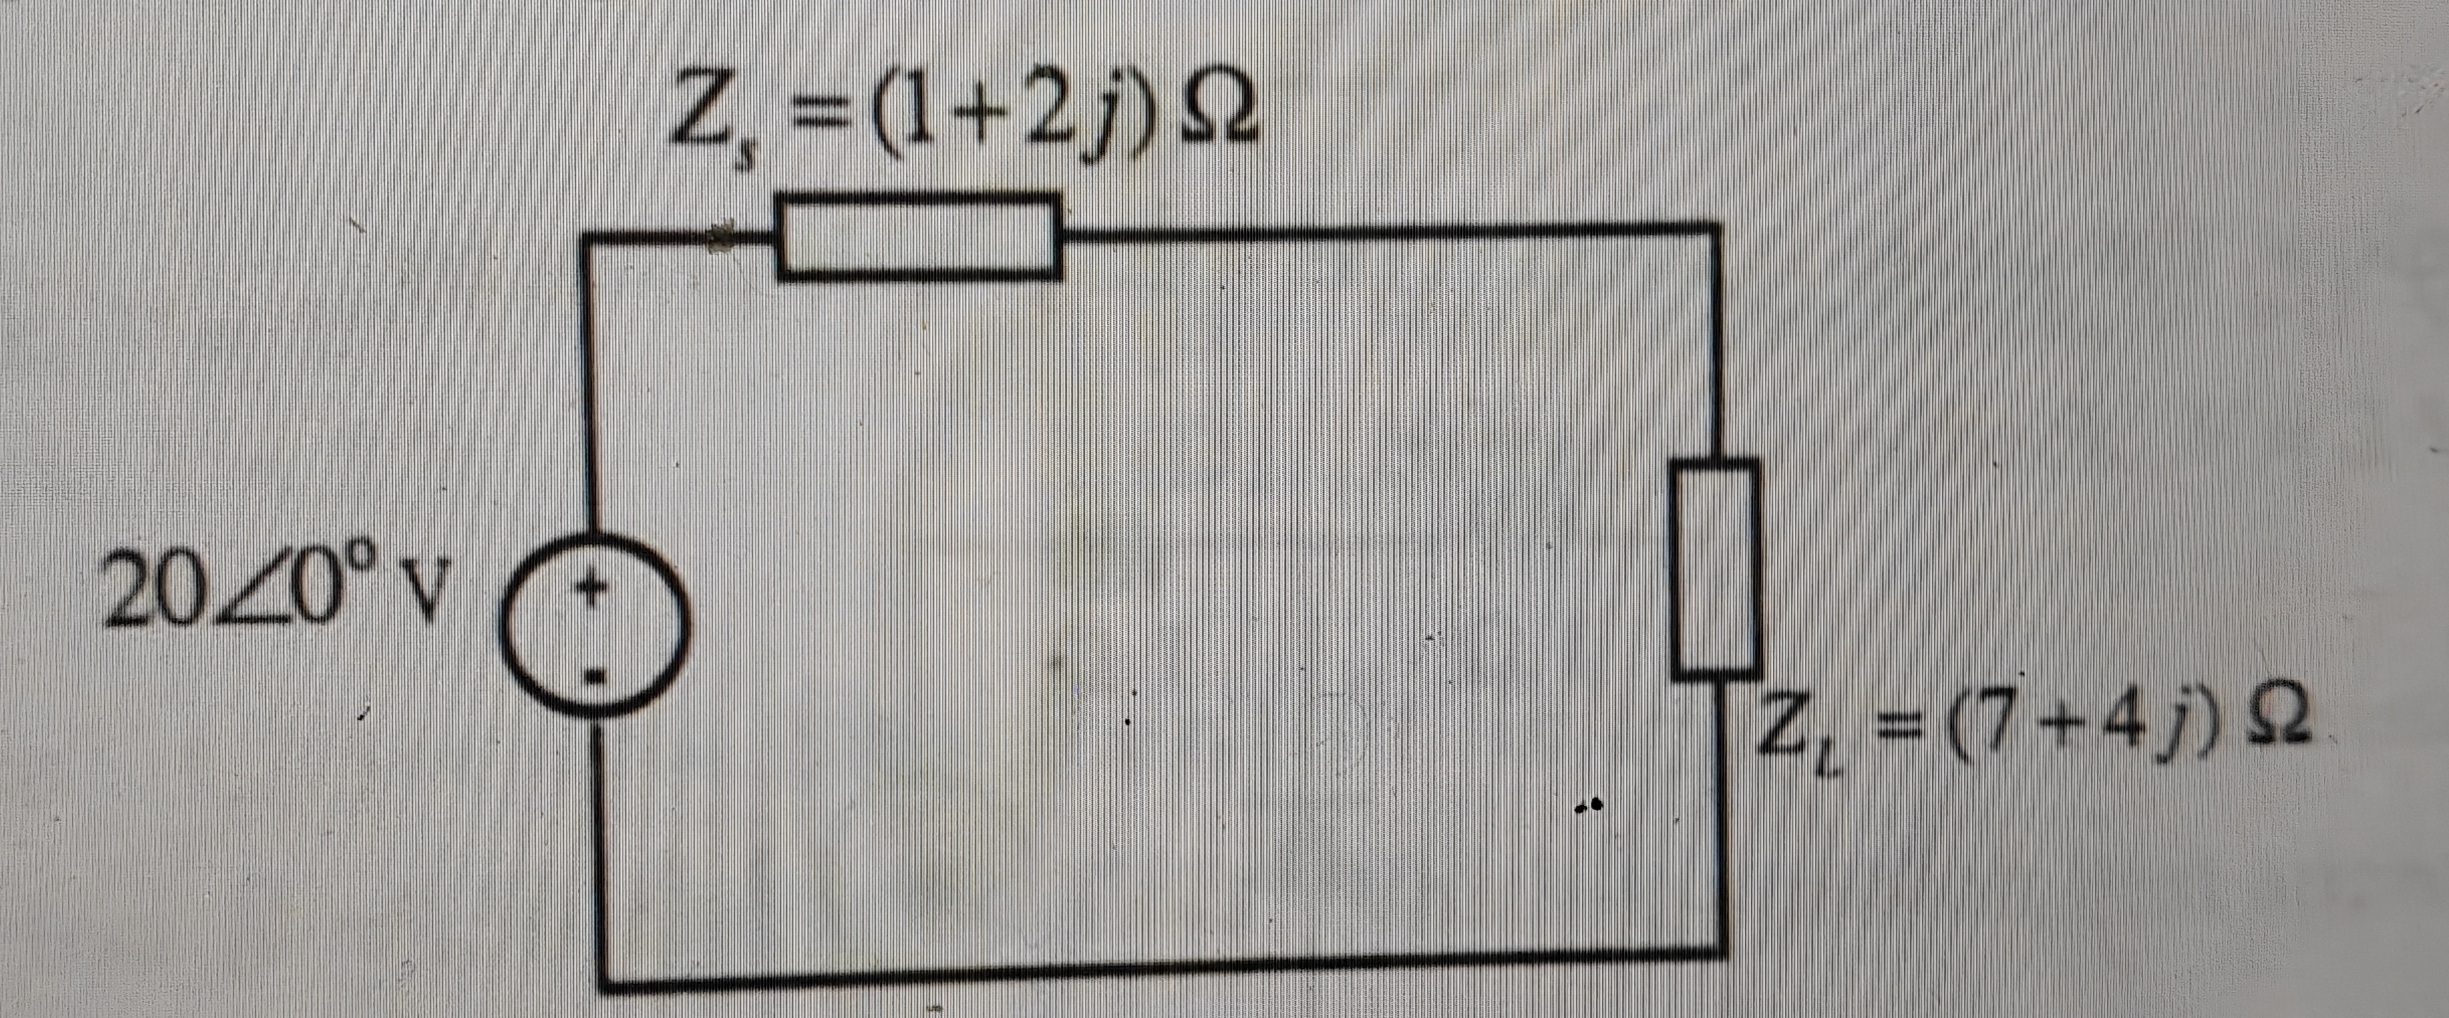
\includegraphics[width=0.5\columnwidth]{figs/fig_9.jpg}
    \caption{\centering Circuit for Q-27}
    \label{fig:placeholder_9}
\end{figure}
\begin{enumerate}
    \begin{multicols}{4}
        \item 8 VAR 
        \item 16 VAR
        \item 28 VAR
        \item 32 VAR
    \end{multicols}
\end{enumerate}
\hfill $\brak{\text{GATE EC 2009}}$

\item The switch in circuit shown was on a position $a$ for a long time, and is moved to positon $b$ at time t=0. The current $i\brak{t}$ for $t>0$ is given by 
\begin{figure}[H]
    \centering
    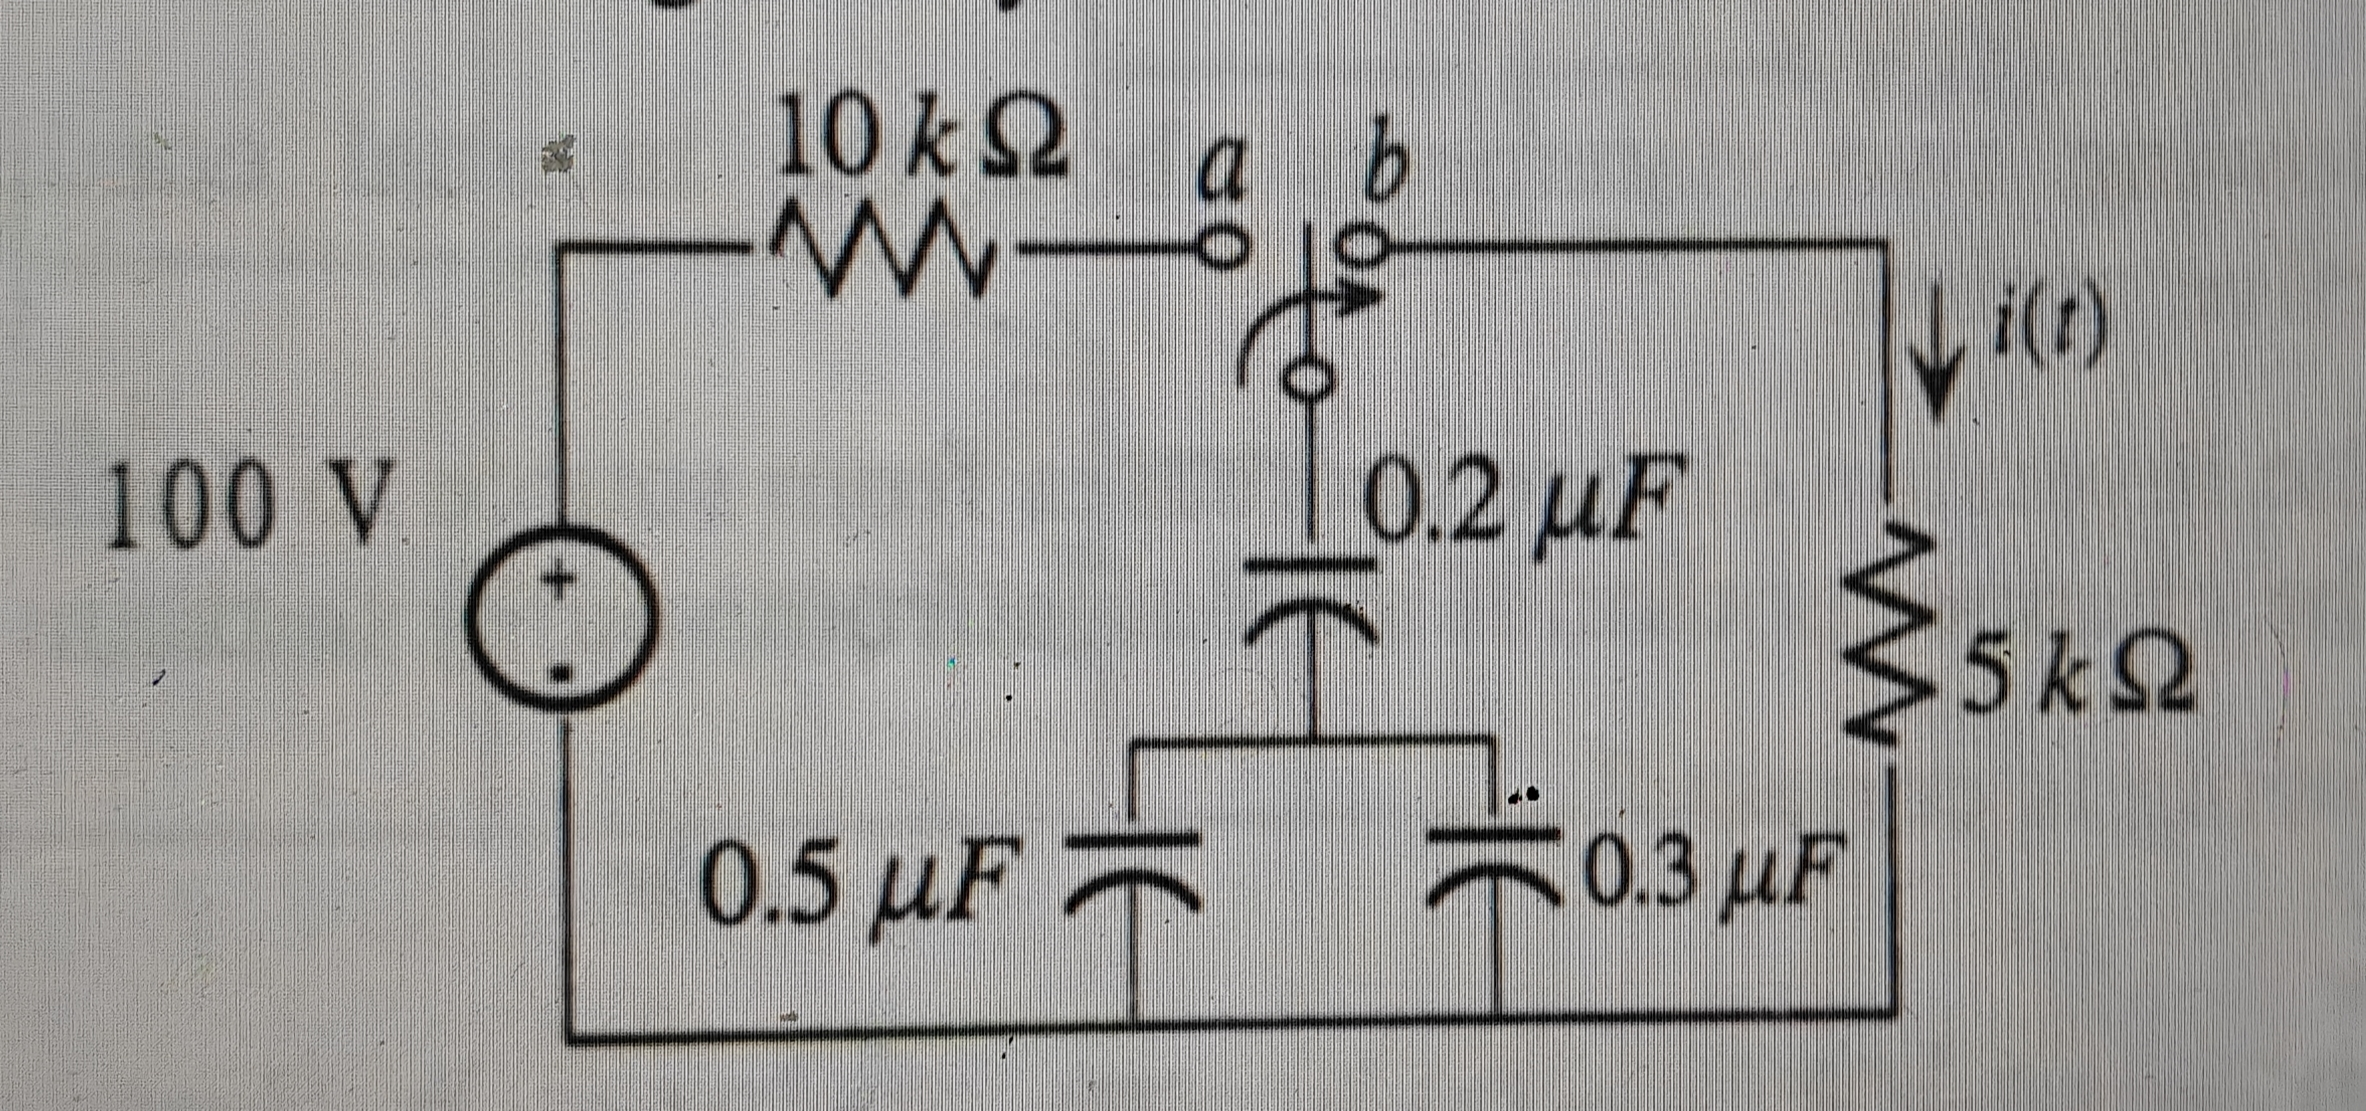
\includegraphics[width=0.5\columnwidth]{figs/fig_10.jpg}
    \caption{\centering Circuit for Q-28}
    \label{fig:placeholder_10}
\end{figure}

\begin{enumerate}
    \begin{multicols}{2}
        \item $0.2e^{-125t}u\brak{t}\quad mA$
        \item $20e^{-1250t}u\brak{t}\quad mA$
        \item $0.2e^{-1250t}u\brak{t}\quad mA$
        \item $20e^{-1000t}u\brak{t}\quad mA$
    \end{multicols}
\end{enumerate}
\hfill $\brak{\text{GATE EC 2009}}$

\item In the $\figref{fig:placeholder_11}$ shown below, what value of $R_l$ maximizes the power delivered to $R_l$ ?
\begin{figure}[H]
    \centering
    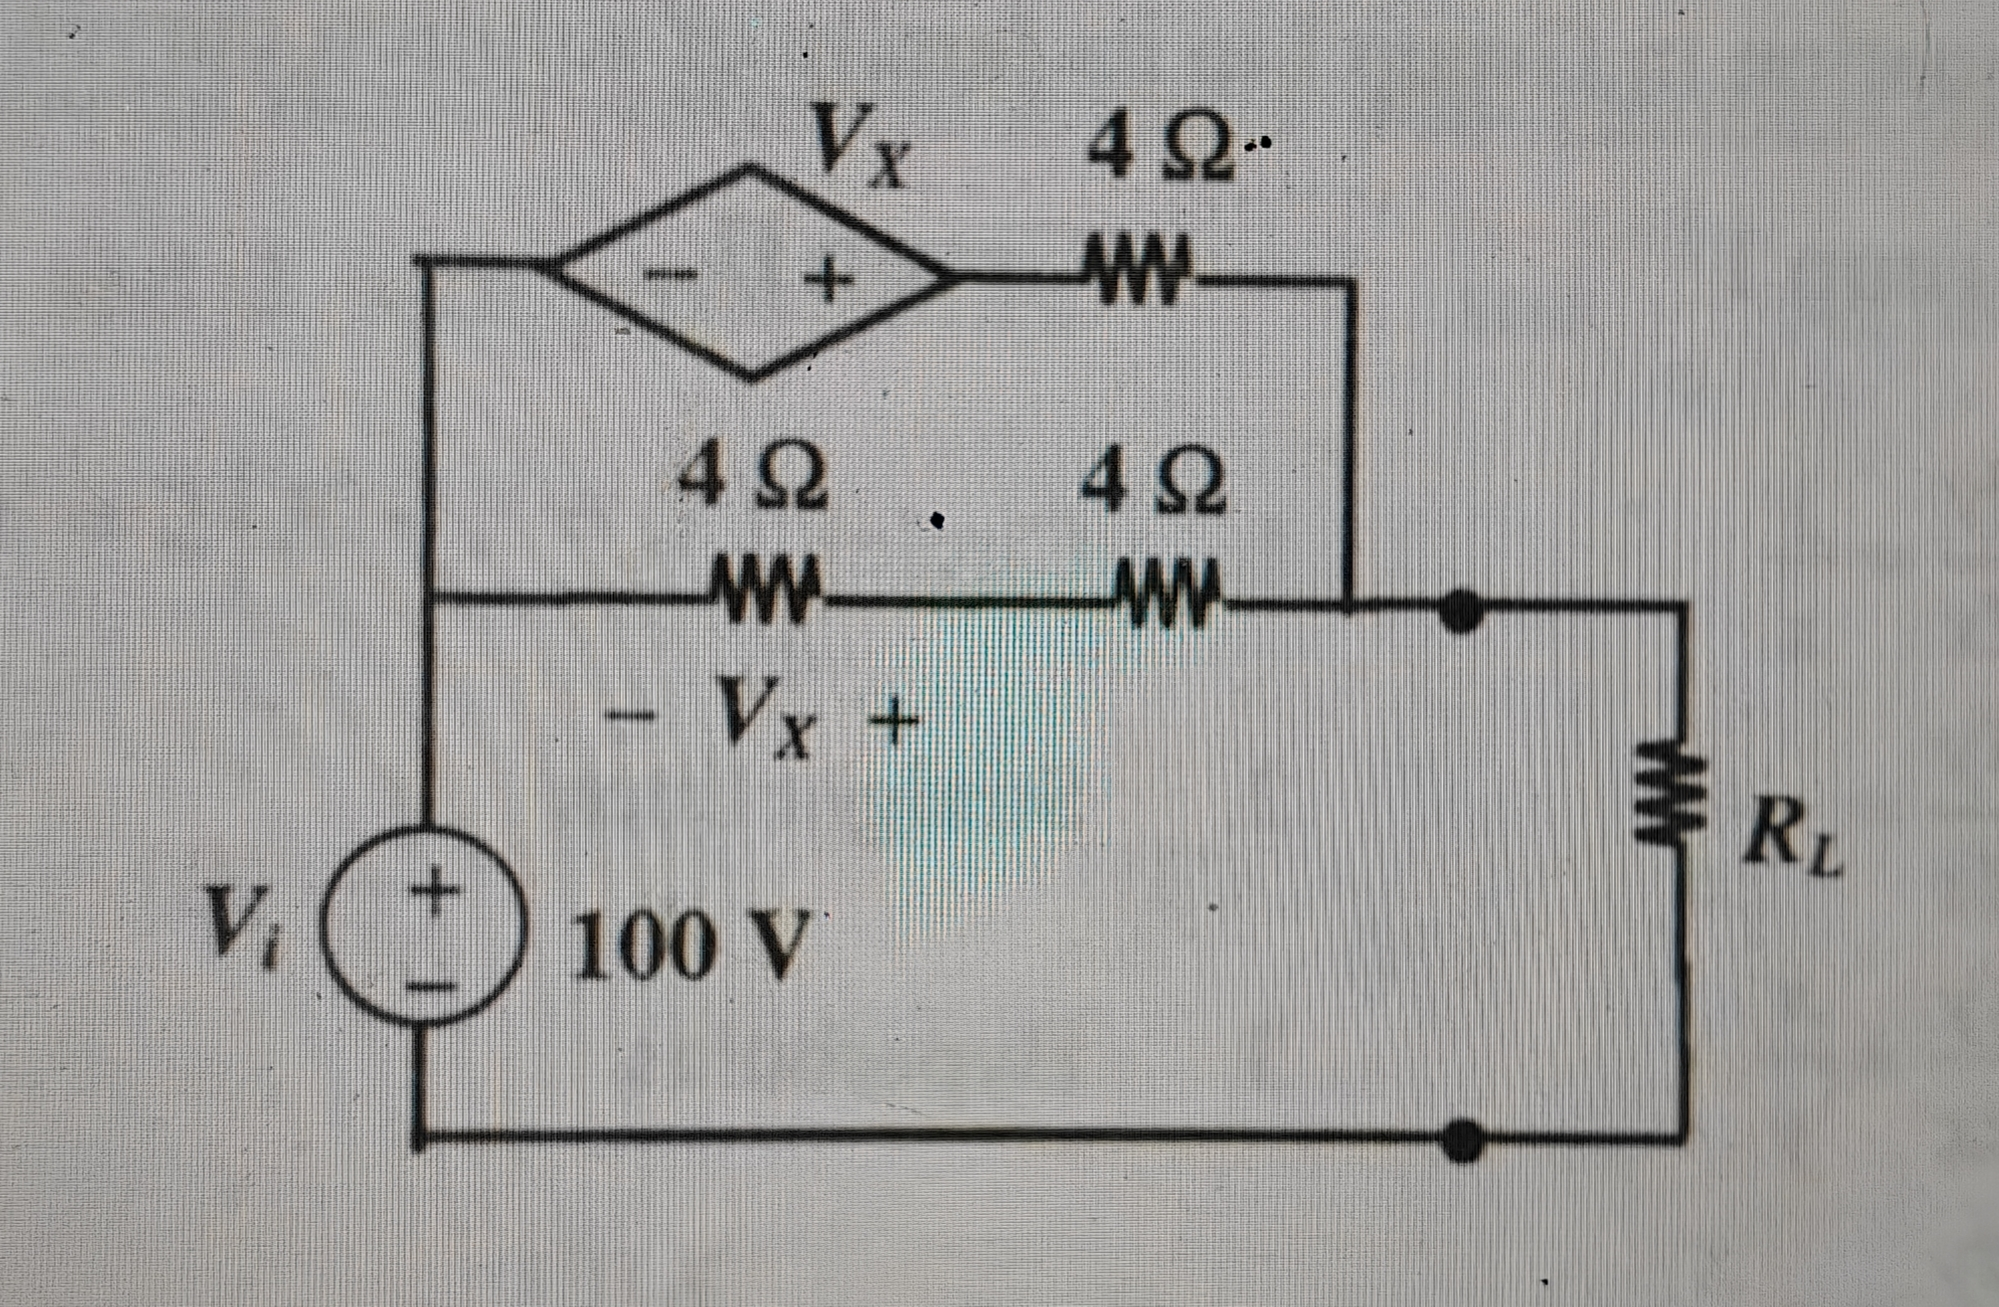
\includegraphics[width=0.5\columnwidth]{figs/fig_11.jpg}
    \caption{\centering Circuit for Q-29}
    \label{fig:placeholder_11}
\end{figure}
\begin{enumerate}
    \begin{multicols}{4}
        \item $2.4 \ohm$
        \item $\frac{8}{3} \ohm$
        \item $4 \ohm$
        \item $6 \ohm$
    \end{multicols}
\end{enumerate}
\hfill $\brak{\text{GATE EC 2009}}$

\item The time domain behavior of an RL circuit is represented by 
\begin{align*} 
 L\frac{di}{dt} + Ri = V_0 \brak{1+ Be^{-\frac{Rt}{L}} \sin t } u\brak{t}
\end{align*}

For an intial current of $i\brak{0} = \frac{V_o}{R}$, the steady state value of current is given by 
\begin{enumerate}
    \begin{multicols}{2}
        \item $2.4 \ohm$
        \item $\frac{8}{3} \ohm$
        \item $4 \ohm$
        \item $6 \ohm$
    \end{multicols}
\end{enumerate}
\hfill $\brak{\text{GATE EC 2009}}$

\item In the $\figref{fig:placeholder_12}$ below, the diode is ideal. The voltage V is given by
\begin{figure}[H]
    \centering
    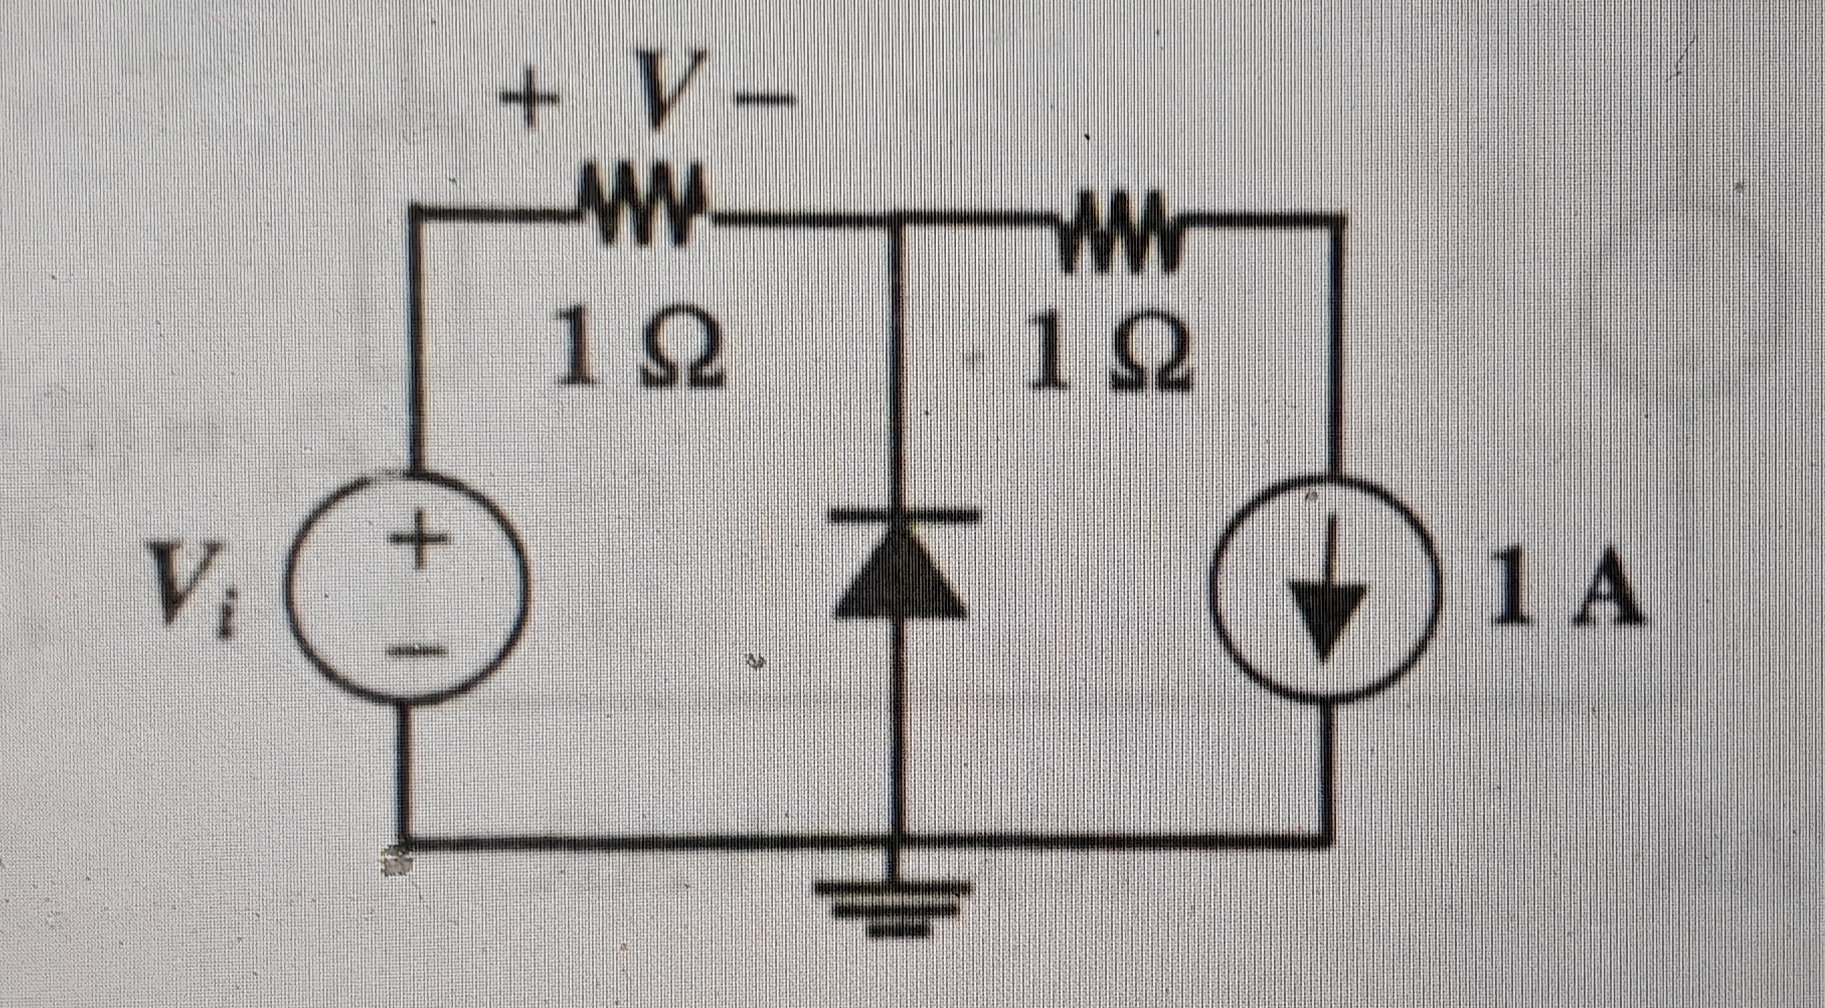
\includegraphics[width=0.5\columnwidth]{figs/fig_12.jpg}
    \caption{\centering Circuit for Q-31}
    \label{fig:placeholder_12}
\end{figure}
\begin{enumerate}
    \begin{multicols}{4}
        \item $min\brak{V_i ,1}$
        \item $max\brak{V_i ,1}$
        \item $min\brak{-V_i ,1}$
        \item $max\brak{-V_i ,1}$
    \end{multicols}
\end{enumerate}
\hfill $\brak{\text{GATE EC 2009}}$

\item Consider the following two statements about the internal conditions in an n-channel MOSFET operating in the active region 
\begin{align*}
    S1: The inversion charge decreases from source to drain
    
    S2: The channel potential increases from source to drain
\end{align*}
Which of the following is correct?
\begin{enumerate}
        \item Only S2 is true
        \item Both S1 and S2 are false.
        \item Both S1 and S2 are true, but S2 is not a reason for S1
        \item Both S1 and S2 are true, but S2 is a reason for S1
\end{enumerate}
\hfill $\brak{\text{GATE EC 2009}}$

\item In the following astable multivibrator circuit, which properties of $v_o(t)$ depend on $R_2$ ?
\begin{figure}[H]
    \centering
    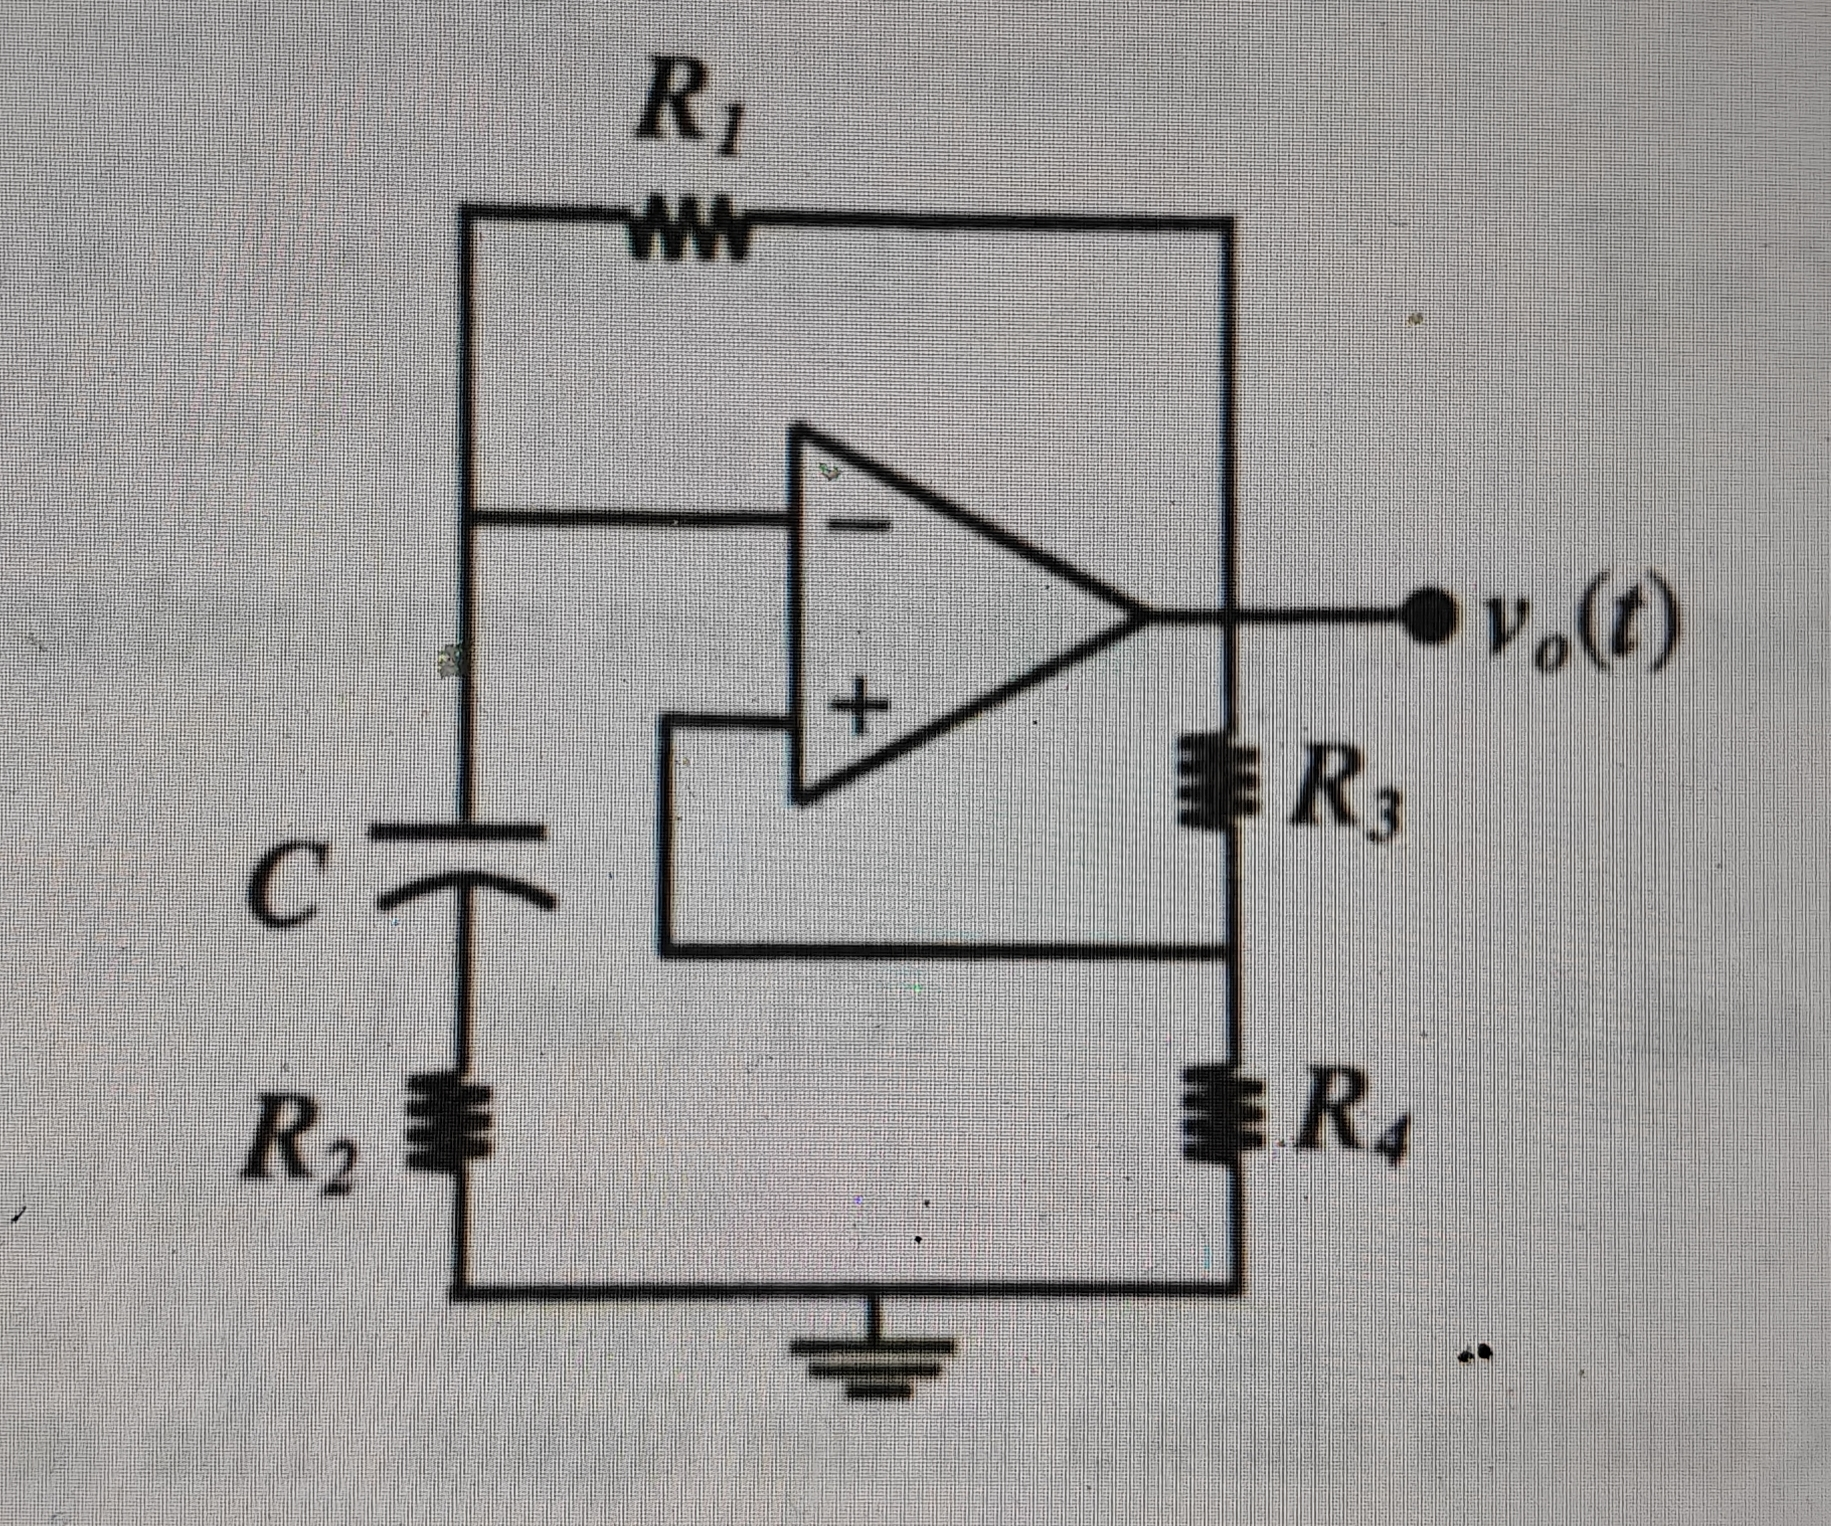
\includegraphics[width=0.5\columnwidth]{figs/fig_13.jpg}
    \caption{\centering Circuit for Q-33}
    \label{fig:placeholder_13}
\end{figure}
\begin{enumerate}
        \item Only the frequency 
        \item Only the amplitude
        \item Both the amplitude and the frequency 
        \item Neither the amplitude and the frequency 
\end{enumerate}
\hfill $\brak{\text{GATE EC 2009}}$

\item In the $\figref{fig:placeholder_14}$ shown below, the op-amp is ideal, the transistor has $V_{BE} = 0.6 V$ and $\beta = 150$. Decide whether the feedback in the circuit is positive or negative and determine the voltage V at the output of op-amp.     
\begin{figure}[H]
    \centering
    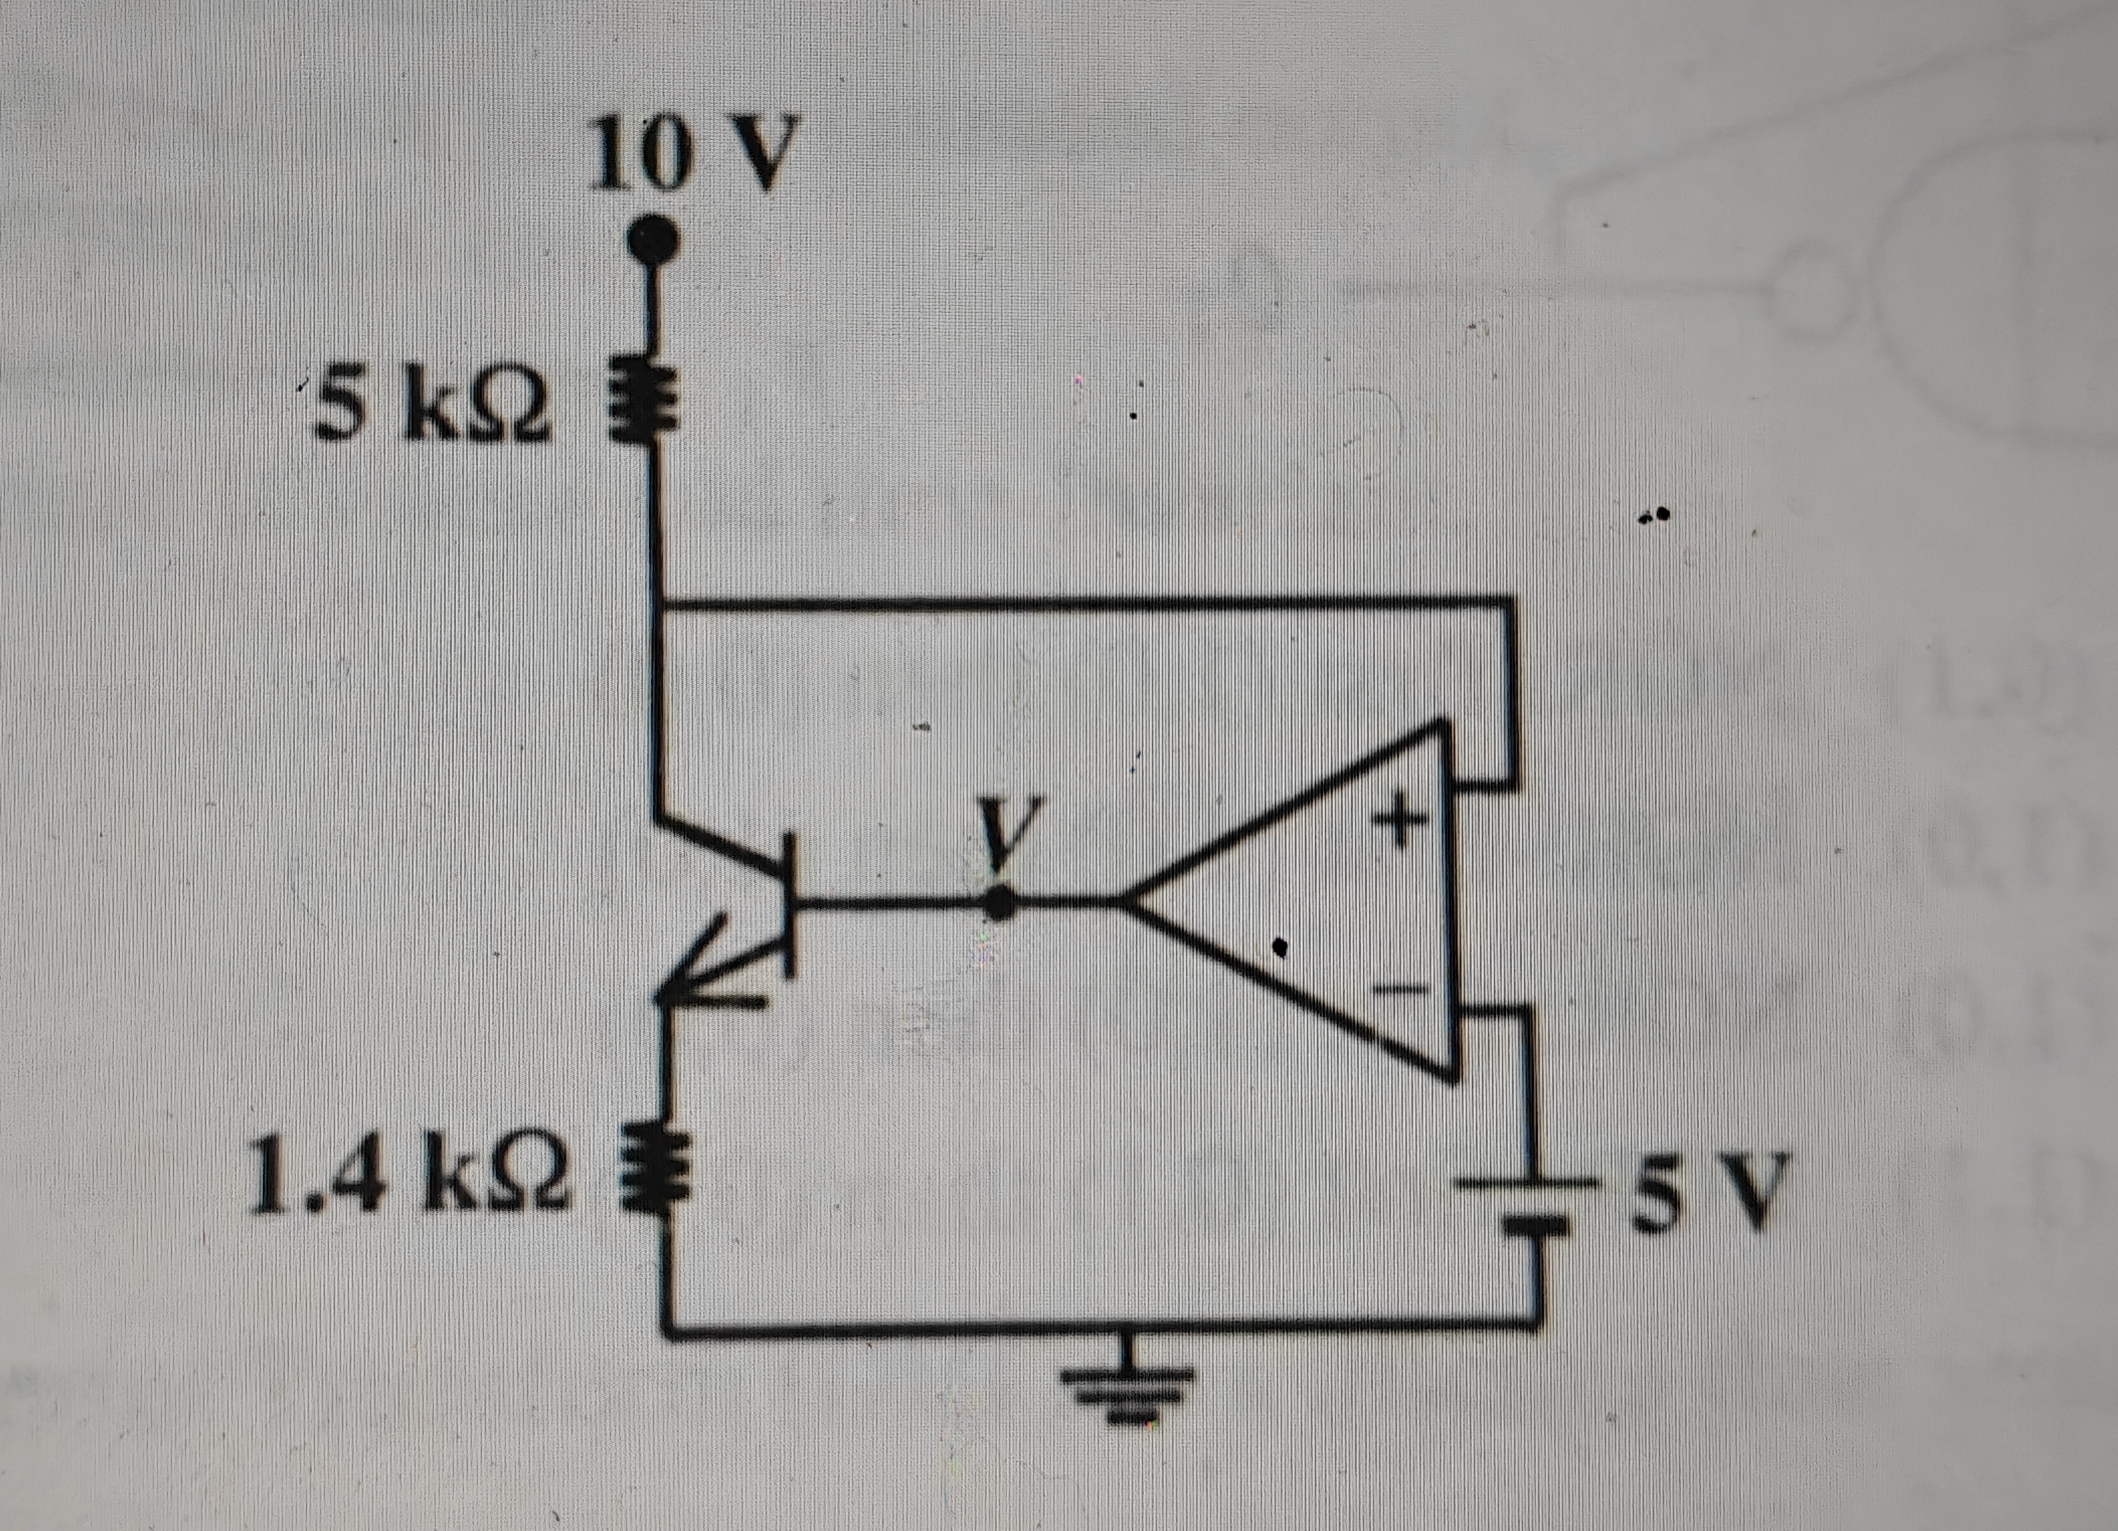
\includegraphics[width=0.5\columnwidth]{figs/fig_14.jpg}
    \caption{\centering Circuit for Q-34}
    \label{fig:placeholder_14}
\end{figure}
\begin{enumerate}
    \begin{multicols}{2}
        \item Positive feedback, $V=10V$
        \item Positive feedback, $V=0V$
        \item Negative feedback, $V=5V$
        \item Negative feedback, $V=2V$
    \end{multicols}
\end{enumerate}
\hfill $\brak{\text{GATE EC 2009}}$

\item A small signal source $v_i\brak{t} = A\cos{20t} + B \sin{10^6t}$ is applied to a transistor amplifier as shown in the $\figref{fig:placeholder_15}$. The transistor has $\beta = 150$ and $h_{ie} = 3k\ohm$. Which expression best approximates $v_o\brak{t} ?$
\begin{figure}[H]
    \centering
    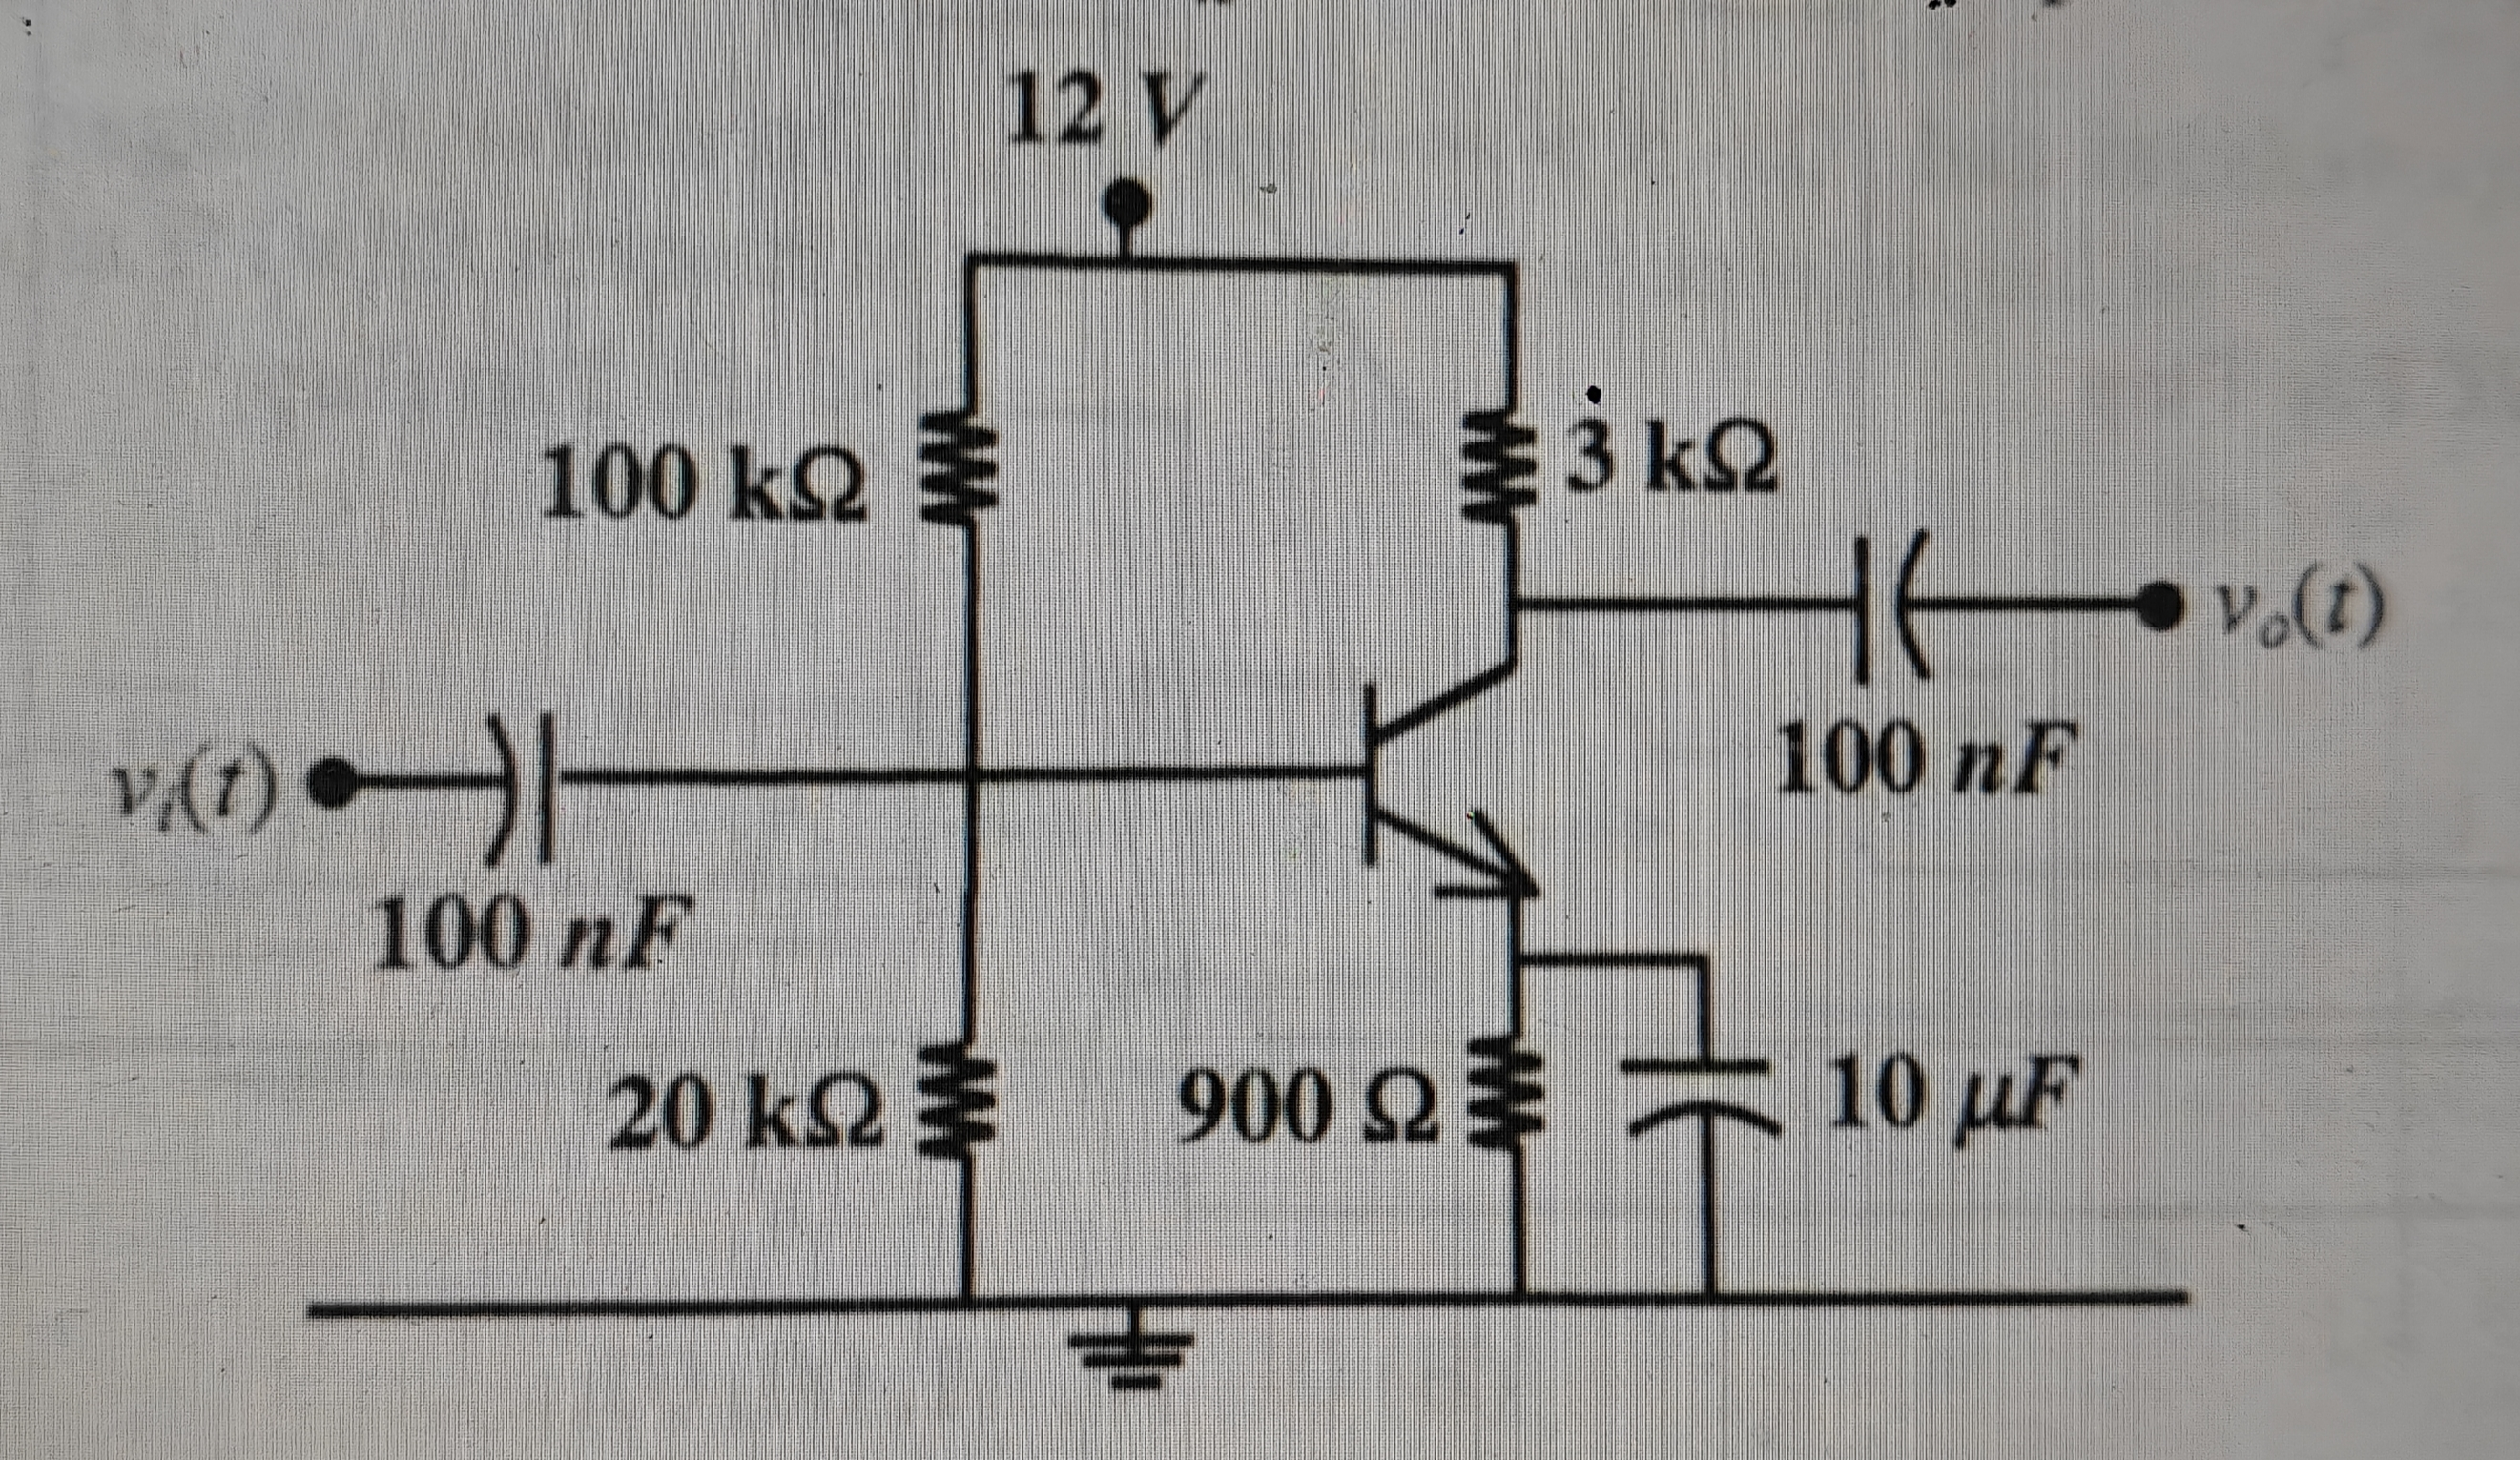
\includegraphics[width=0.5\columnwidth]{figs/fig_15.jpg}
    \caption{\centering Circuit for Q-35}
    \label{fig:placeholder_15}
\end{figure}
\begin{enumerate}
    \begin{multicols}{2}
        \item $v_o\brak{t} = -1500\brak{A\cos{20t} + B \sin{10^6t}}$
        \item $v_o\brak{t} = -150\brak{A\cos{20t} + B \sin{10^6t}}$
        \item $v_o\brak{t} = -1500B \sin{10^6t}$
        \item $v_o\brak{t} = -150B \sin{10^6t}$
    \end{multicols}
\end{enumerate}
\hfill $\brak{\text{GATE EC 2009}}$

\item If $X=1$ in the logic equation $\sbrak{X + Z\cbrak{\overline{Y} + \brak{\overline{Z} + X\overline{Y}}}} \cbrak{\overline{X} + \overline{Z}\brak{X+Y}} = 1$, then
\begin{enumerate}
    \begin{multicols}{4}
        \item $Y = Z$
        \item $Y = \overline{Z}$
        \item $Z=1$
        \item $Z=0$
    \end{multicols}
\end{enumerate}
\hfill $\brak{\text{GATE EC 2009}}$

\item What are the minimum numbers of 2-to-1 multiplexers recquired to generate a 2-input AND gate and a 2-input Ex-OR gate ?
\begin{enumerate}
    \begin{multicols}{4}
        \item 1 and 2
        \item 1 and 3
        \item 1 and 1
        \item 2 and 2
    \end{multicols}
\end{enumerate}
\hfill $\brak{\text{GATE EC 2009}}$

\item Refer to NAND and NOR latches shown in the $\figref{fig:placeholder_16}$. The inputs $\brak{P_1,P_2}$ for both the latches are first made $\brak{0,1}$ and then, after a few seconds, made $\brak{1,1}$. The corresponding stable outputs $\brak{Q_1, Q_2}$ are
\begin{figure}[H]
    \centering
    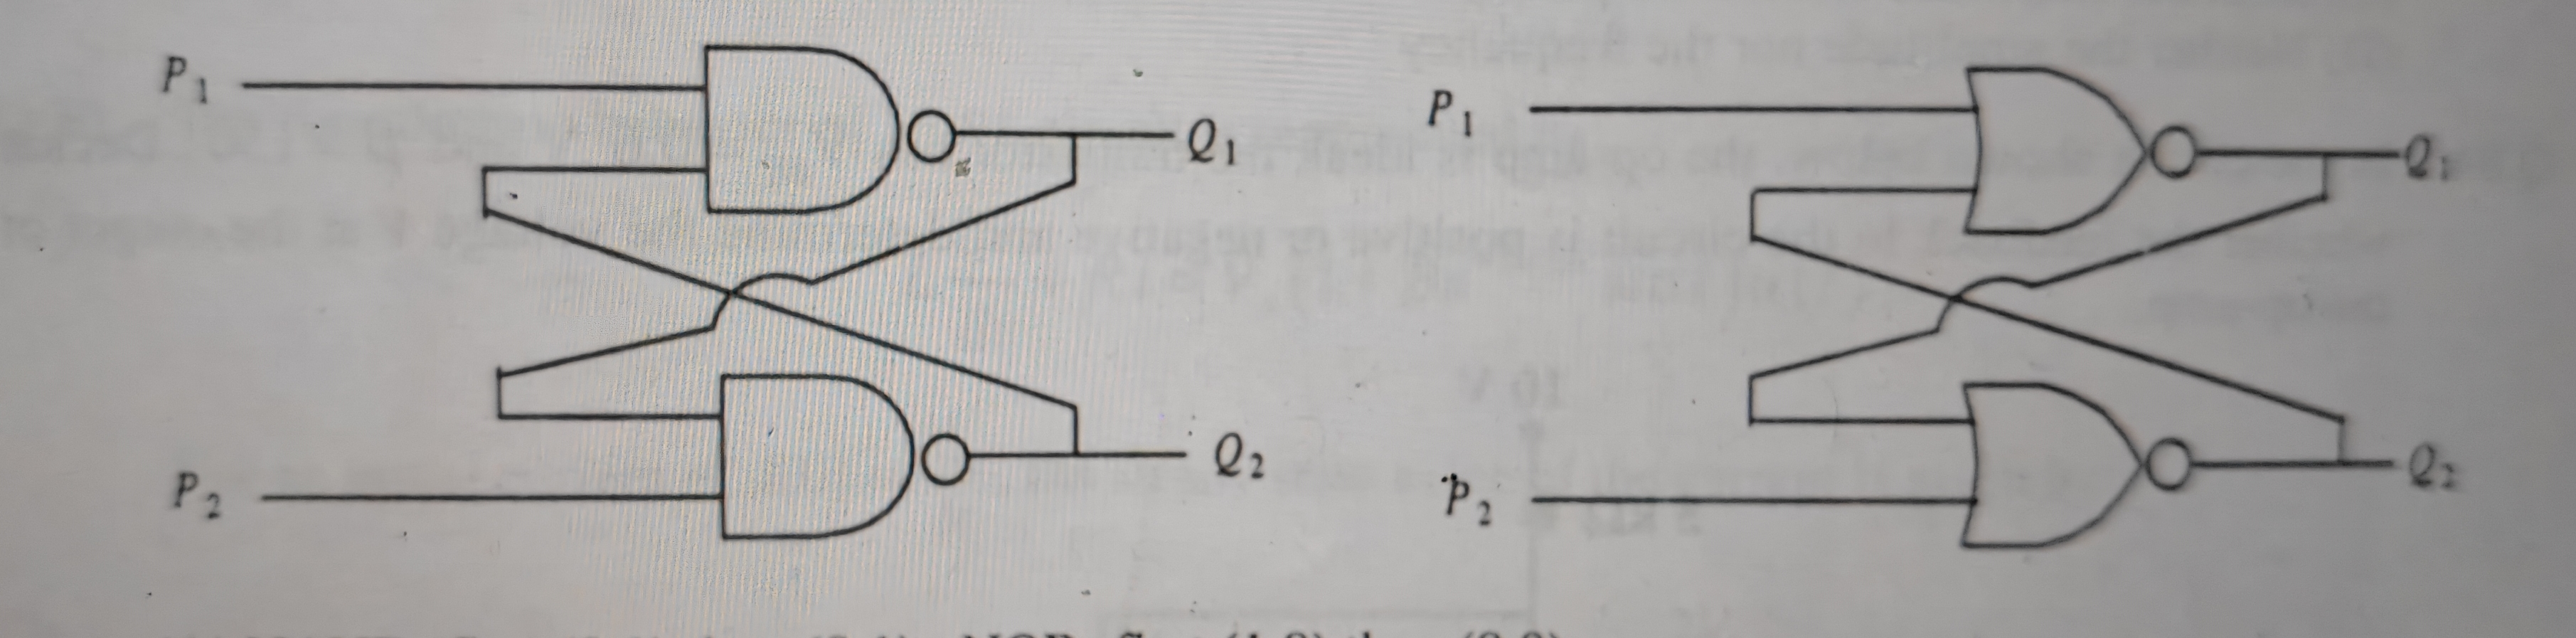
\includegraphics[width=0.5\columnwidth]{figs/fig_16.jpg}
    \caption{\centering NAND and NOR latches}
    \label{fig:placeholder_16}
\end{figure}
\begin{enumerate}
    \item NAND: first $\brak{0,1}$ then $\brak{0,1}$   NOR: first $\brak{1,0}$ then $\brak{0,0}$
    \item NAND: first $\brak{1,0}$ then $\brak{1,0}$   NOR: first $\brak{1,0}$ then $\brak{1,0}$
    \item NAND: first $\brak{1,0}$ then $\brak{1,0}$   NOR: first $\brak{1,0}$ then $\brak{0,0}$
    \item NAND: first $\brak{1,0}$ then $\brak{1,1}$   NOR: first $\brak{0,1}$ then $\brak{0,1}$
\end{enumerate}
\hfill $\brak{\text{GATE EC 2009}}$

\item What are the counting states $(Q_1, Q_2)$ for the counter shown in the figure below ?
\begin{figure}[H]
    \centering
    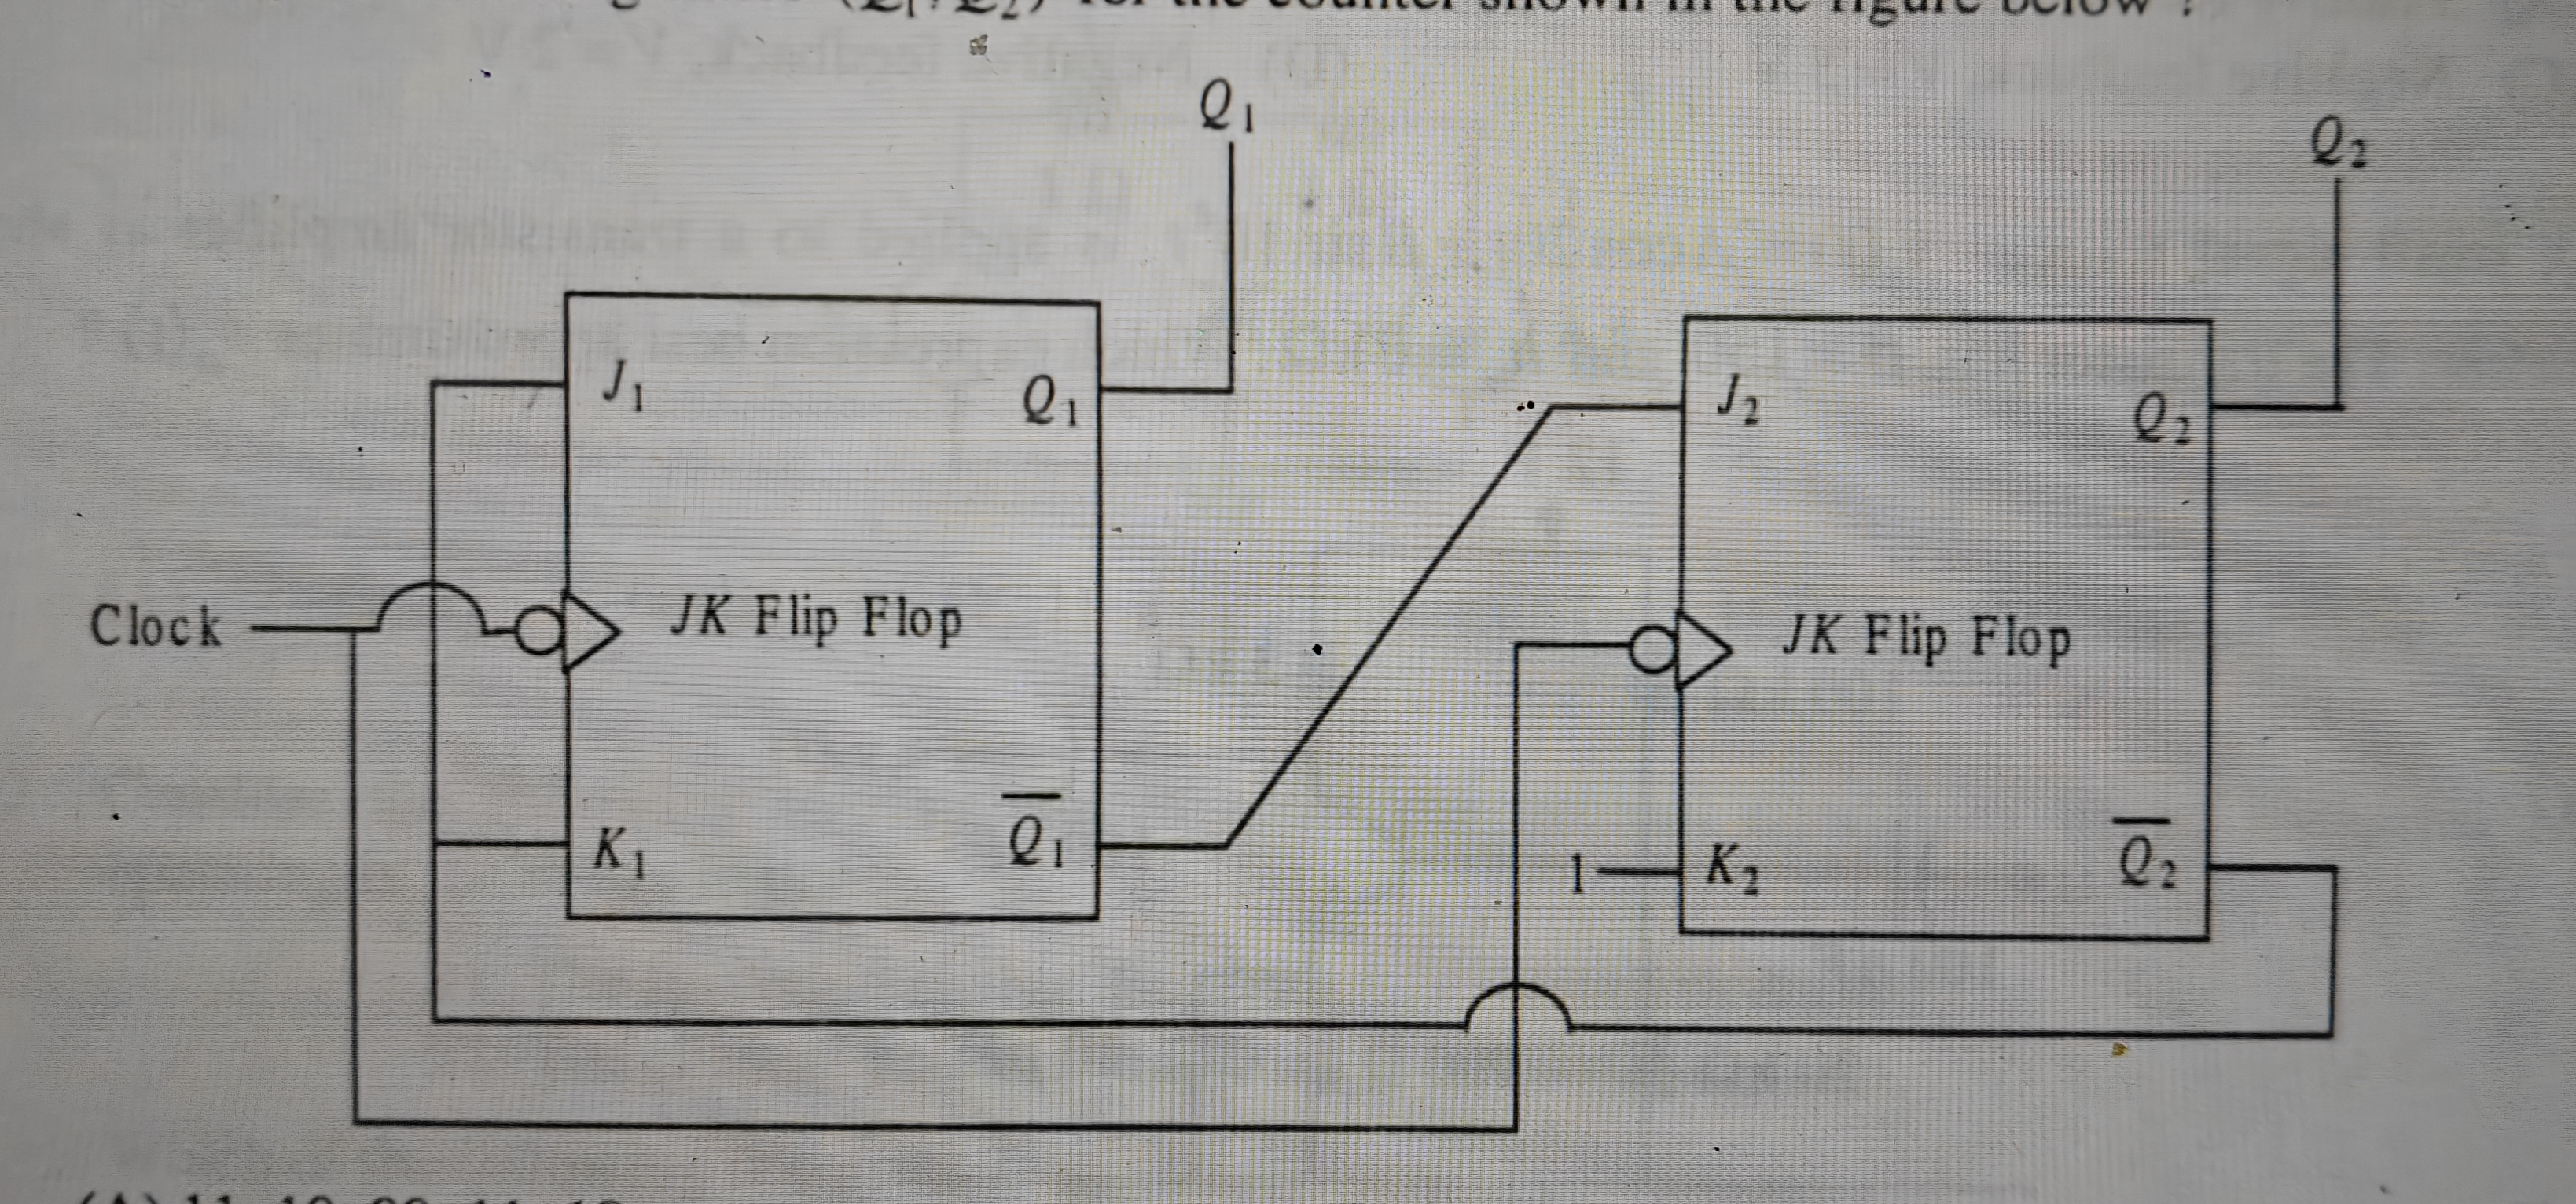
\includegraphics[width=0.5\columnwidth]{figs/fig_17.jpg}
    \caption{\centering Figure for Q-39}
    \label{fig:placeholder_17}
\end{figure}
\begin{enumerate}
    \begin{multicols}{2}
        \item 11, 10, 00, 11, 10, ...
        \item 01, 10, 11, 00, 01, ...
        \item 00, 11, 01, 10, 00, ...
        \item 01, 10, 00, 01, 10, ...
    \end{multicols}
\end{enumerate}
\hfill $\brak{\text{GATE EC 2009}}$

\item A system with transfer function $H\brak{z}$ has impulse response $h\brak{\cdot}$ defined as $h\brak{2}=1$, h\brak{3}=-1 and h\brak{k}=0 otherwise. Consider the following statements.
\begin{align*}

    S1: H\brak{z} is a low-pass filter.
    
    S2: H\brak{z} is a FIR filter.
\end{align*}
Which of the following is correct?
\begin{enumerate}
        \item Only S2 is true
        \item Both S1 and S2 are false.
        \item Both S1 and S2 are true, but S2 is a reason for S1
        \item Both S1 and S2 are true, but S2 is not a reason for S1
\end{enumerate}
\hfill $\brak{\text{GATE EC 2009}}$

\item Consider a system whose input $x$ and output $y$ are related by the equation 
\begin{align*}
    y(t)= \int_{-\infty}^{\infty} x(t-\tau)h(2\tau)d\tau
\end{align*}
where h(t) is shown in the $\figref{fig:placeholder_18}$.
\begin{figure}[H]
    \centering
    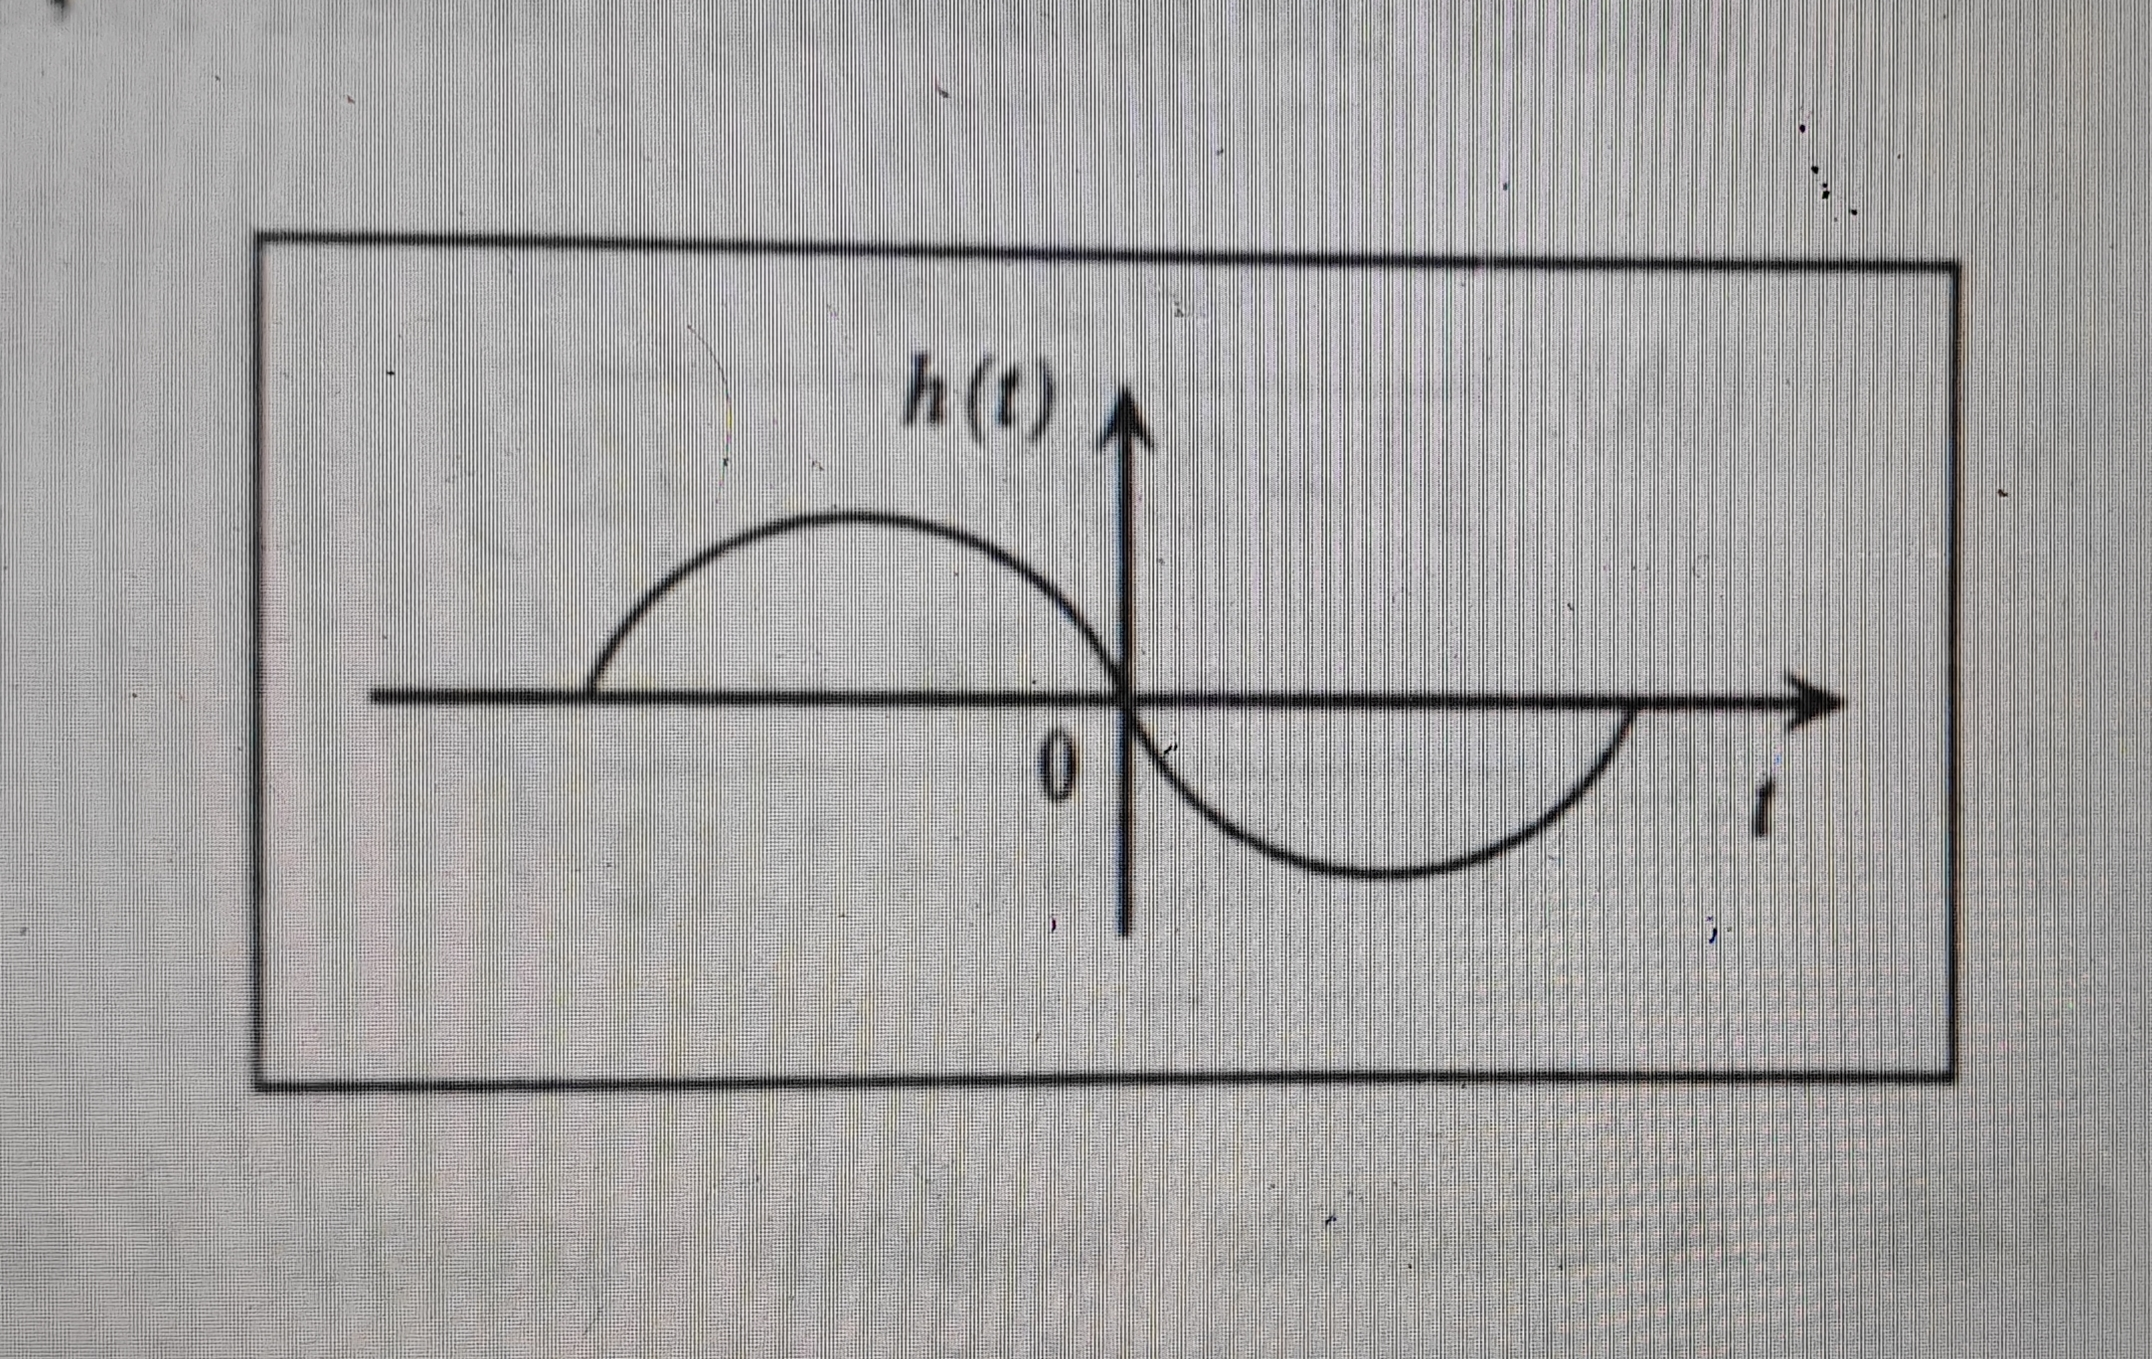
\includegraphics[width=0.5\columnwidth]{figs/fig_18.jpg}
    \caption{\centering Figure for Q-41}
    \label{fig:placeholder_18}
\end{figure}

Which of the following four properties are possessed by the system?

BIBO: Bounded input gives a bounded output.

Casual: The system is casual.

LP: The system is low-pass

LTI: The system is linear and time-invariant.
\begin{enumerate}
    \begin{multicols}{2}
        \item Casual, LP
        \item BIBO, LTI
        \item BIBO, LTI, Casual
        \item LP, LTI
    \end{multicols}
\end{enumerate}
\hfill $\brak{\text{GATE EC 2009}}$

\item The 4-point Discrete Fourier Transform $\brak{DFT}$ of a discrete time sequence $\cbrak{1,0,2,3}$ is 
\begin{enumerate}
    \begin{multicols}{2}
        \item $\sbrak{0,-2+2j, 2,-2,-2j}$
        \item $\sbrak{2,2+2j, 6, 2-2j}$
        \item $\sbrak{6,1-3j, 2, 1+3j}$
        \item $\sbrak{6,-1+3j, 0,-1-3j}$
    
    \end{multicols}
\end{enumerate}
\hfill $\brak{\text{GATE EC 2009}}$

\item The feedback configuration and pole-zero locations of $G(s) = \frac{s^2 -2s +2}{s^2 +2s +2}$ are shown below in the $\figref{fig:placeholder_19}$. The root locus for $\textbf{negative}$ values of k, i.e. for $-\infty < k<0$, has breakway/break-in points and angles of departure at pole $\textbf{P}$ $\brak{\text{with respect to the positive real axis}}$ equal to 
\begin{figure}[H]
    \centering
    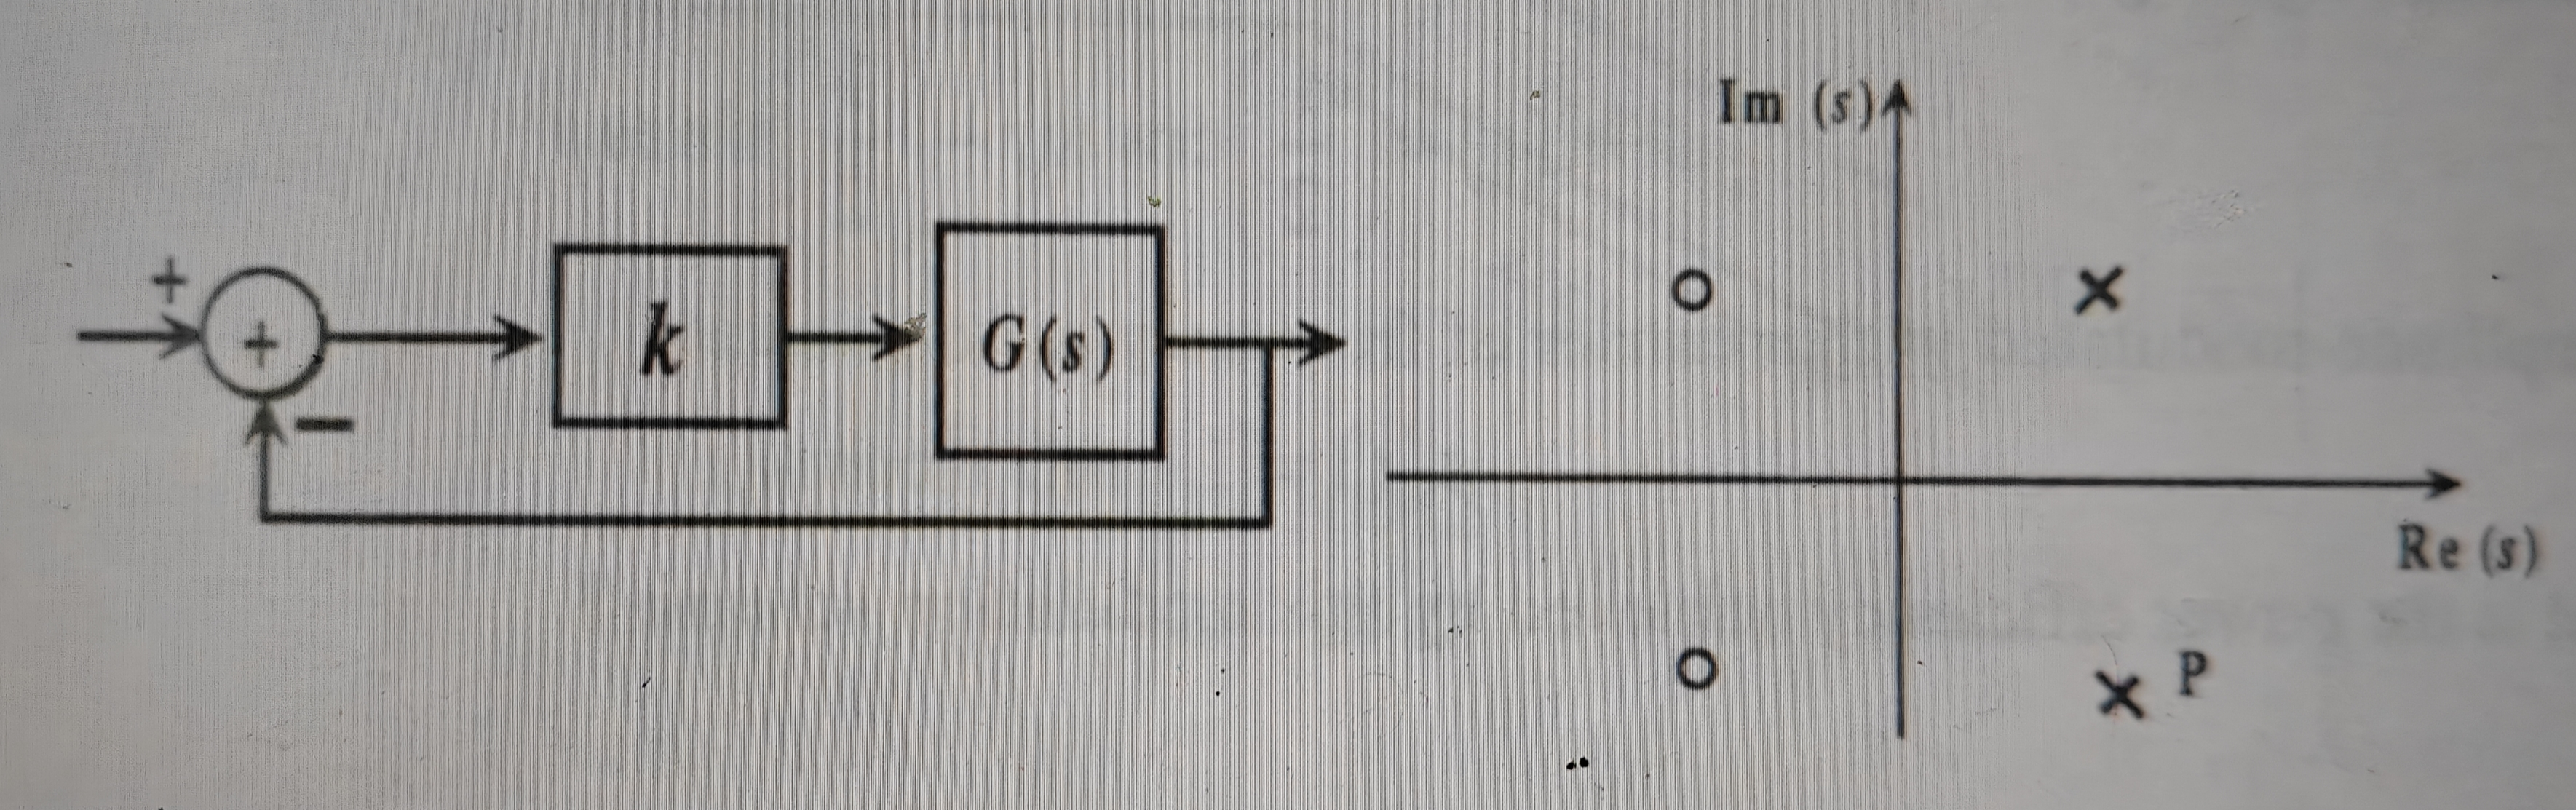
\includegraphics[width=0.5\columnwidth]{figs/fig_19.jpg}
    \caption{\centering Figure for Q-43}
    \label{fig:placeholder_19}
\end{figure}
\begin{enumerate}
    \begin{multicols}{4}
        \item $\pm \sqrt{2}\quad and \quad  0^{\degree}$
        \item $\pm \sqrt{2}\quad and \quad  45^{\degree}$
        \item $\pm \sqrt{3}\quad and \quad  0^{\degree}$
        \item $\pm \sqrt{3}\quad and \quad  45^{\degree}$
    \end{multicols}
\end{enumerate}
\hfill $\brak{\text{GATE EC 2009}}$


\item An LTI system having transfer function $\frac{s^2+1}{s^2 +2s +1}$ and input $x\brak{t} = \sin\brak{t+1}$ is in steady state. The output is sampled at the rate $\omega_s rad/s$ to obtain the final output $\cbrak{ y\brak{k}}$. Which of the following is true?
\begin{enumerate}
        \item $y\brak{\cdot}$ is zero for all sampling frequencies $\omega_s$
        \item $y\brak{\cdot}$ is nonzero for all sampling frequencies $\omega_s$
        \item $y\brak{\cdot}$ is nonzero for $\omega_s>2$, but zero for $\omega_s<2$
        \item $y\brak{\cdot}$ is zero for $\omega_s>2$, but nonzero for $\omega_s<2$
\end{enumerate}
\hfill $\brak{\text{GATE EC 2009}}$

\item The unit step response of an under-damped second order system has steady state value of -2. Which of the following transfer functions has these properties?
\begin{enumerate}
    \begin{multicols}{2}
        \item $\frac{-2.24}{s^2 + 2.59 s +1.12}$
        \item $\frac{-3.82}{s^2 + 1.91 s +1.91}$
        \item $\frac{-2.24}{s^2 - 2.59 s +1.12}$
        \item $\frac{-2.24}{s^2 - 1.91 s +1.91}$
    \end{multicols}
\end{enumerate}
\hfill $\brak{\text{GATE EC 2009}}$

\item A discrete random variable X takes values from 1 to 5 with probabilities as shown in the table. A student calculates the mean of X as 3.5 and her teacher calculates the variance pf X as 1.5 .Which of the following statements are true?
\begin{align*}
\begin{tabular}{|c|c|c|c|c|c|}
\hline
$k$ & 1 & 2 & 3 & 4 & 5 \\
\hline
$P\brak{X = k}$ & 0.1 & 0.2 & 0.4 & 0.2 & 0.1 \\
\hline
\end{tabular}
\end{align*}
\begin{enumerate}
        \item Both the student and the teacher are right
        \item Both the student and the teacher are wrong
        \item The student is wrong but the teacher is right 
        \item The student is right but the teacher is wrong
\end{enumerate}
\hfill $\brak{\text{GATE EC 2009}}$

\item A message signal given by $m\brak{t}=\brak{\frac{1}{2}}\cos{\omega_1t}-\brak{\frac{1}{2}}\sin{\omega_2t}$   is amplitude-modulated with a carrier of frequency $\omega_c$ to generate $s\brak{t}=\sbrak{1+m\brak{t}}\cos\omega_ct$ 

What is the power efficiency achieved by this modulation scheme?
\begin{enumerate}
    \begin{multicols}{2}
        \item $8.33\%$
        \item $11.11\%$
        \item $20\%$
        \item $25\%$
    \end{multicols}
\end{enumerate}
\hfill $\brak{\text{GATE EC 2009}}$

\item A communication channel with AGWN operating at a signal to noise ratio $SNR>>1$ and bandwidth B has capacity $C_1$. If SNR is doubled keeping B constant, the resulting capacity $C_2$ is given by 
\begin{enumerate}
        \item $C_2 \approx 2 C_1$
        \item $C_2 \approx  C_1+B$
        \item $C_2 \approx  C_1 + 2B$
        \item $C_2 \approx  C_1+ 0.3B$
\end{enumerate}
\hfill $\brak{\text{GATE EC 2009}}$

\item A magnetic field in air is measured to be $\vec{B} = B_0(\frac{x}{x^2+y^2} \hat{y} - \frac{y}{x^2+y^2} \hat{x})$

What current distribution leads to this field? 
\begin{enumerate}
        \item $\vec{J}= -\frac{B_o \hat{z}}{\mu_0} \brak{ \frac{1}{x^2 + y^2}}, r \neq 0$
        \item $\vec{J}= -\frac{B_o \hat{z}}{\mu_0} \brak{ \frac{2}{x^2 + y^2}}, r \neq 0$
        \item $\vec{J}= 0, r\neq 0$
        \item $\vec{J}= \frac{B_o \hat{z}}{\mu_0} \brak{ \frac{1}{x^2 + y^2}}, r \neq 0$
\end{enumerate}
\hfill $\brak{\text{GATE EC 2009}}$

\item A transmission line terminates in two branches, each of length $\lambda/4$, as shown. The branches are terminated by $50 \ohm$ loads. The lines are lossless and have characteristic impedances shown in the $\figref{fig:placeholder_21}$. Determine the impedance $Z_i$ as seen by the source.
\begin{figure}[H]
    \centering
    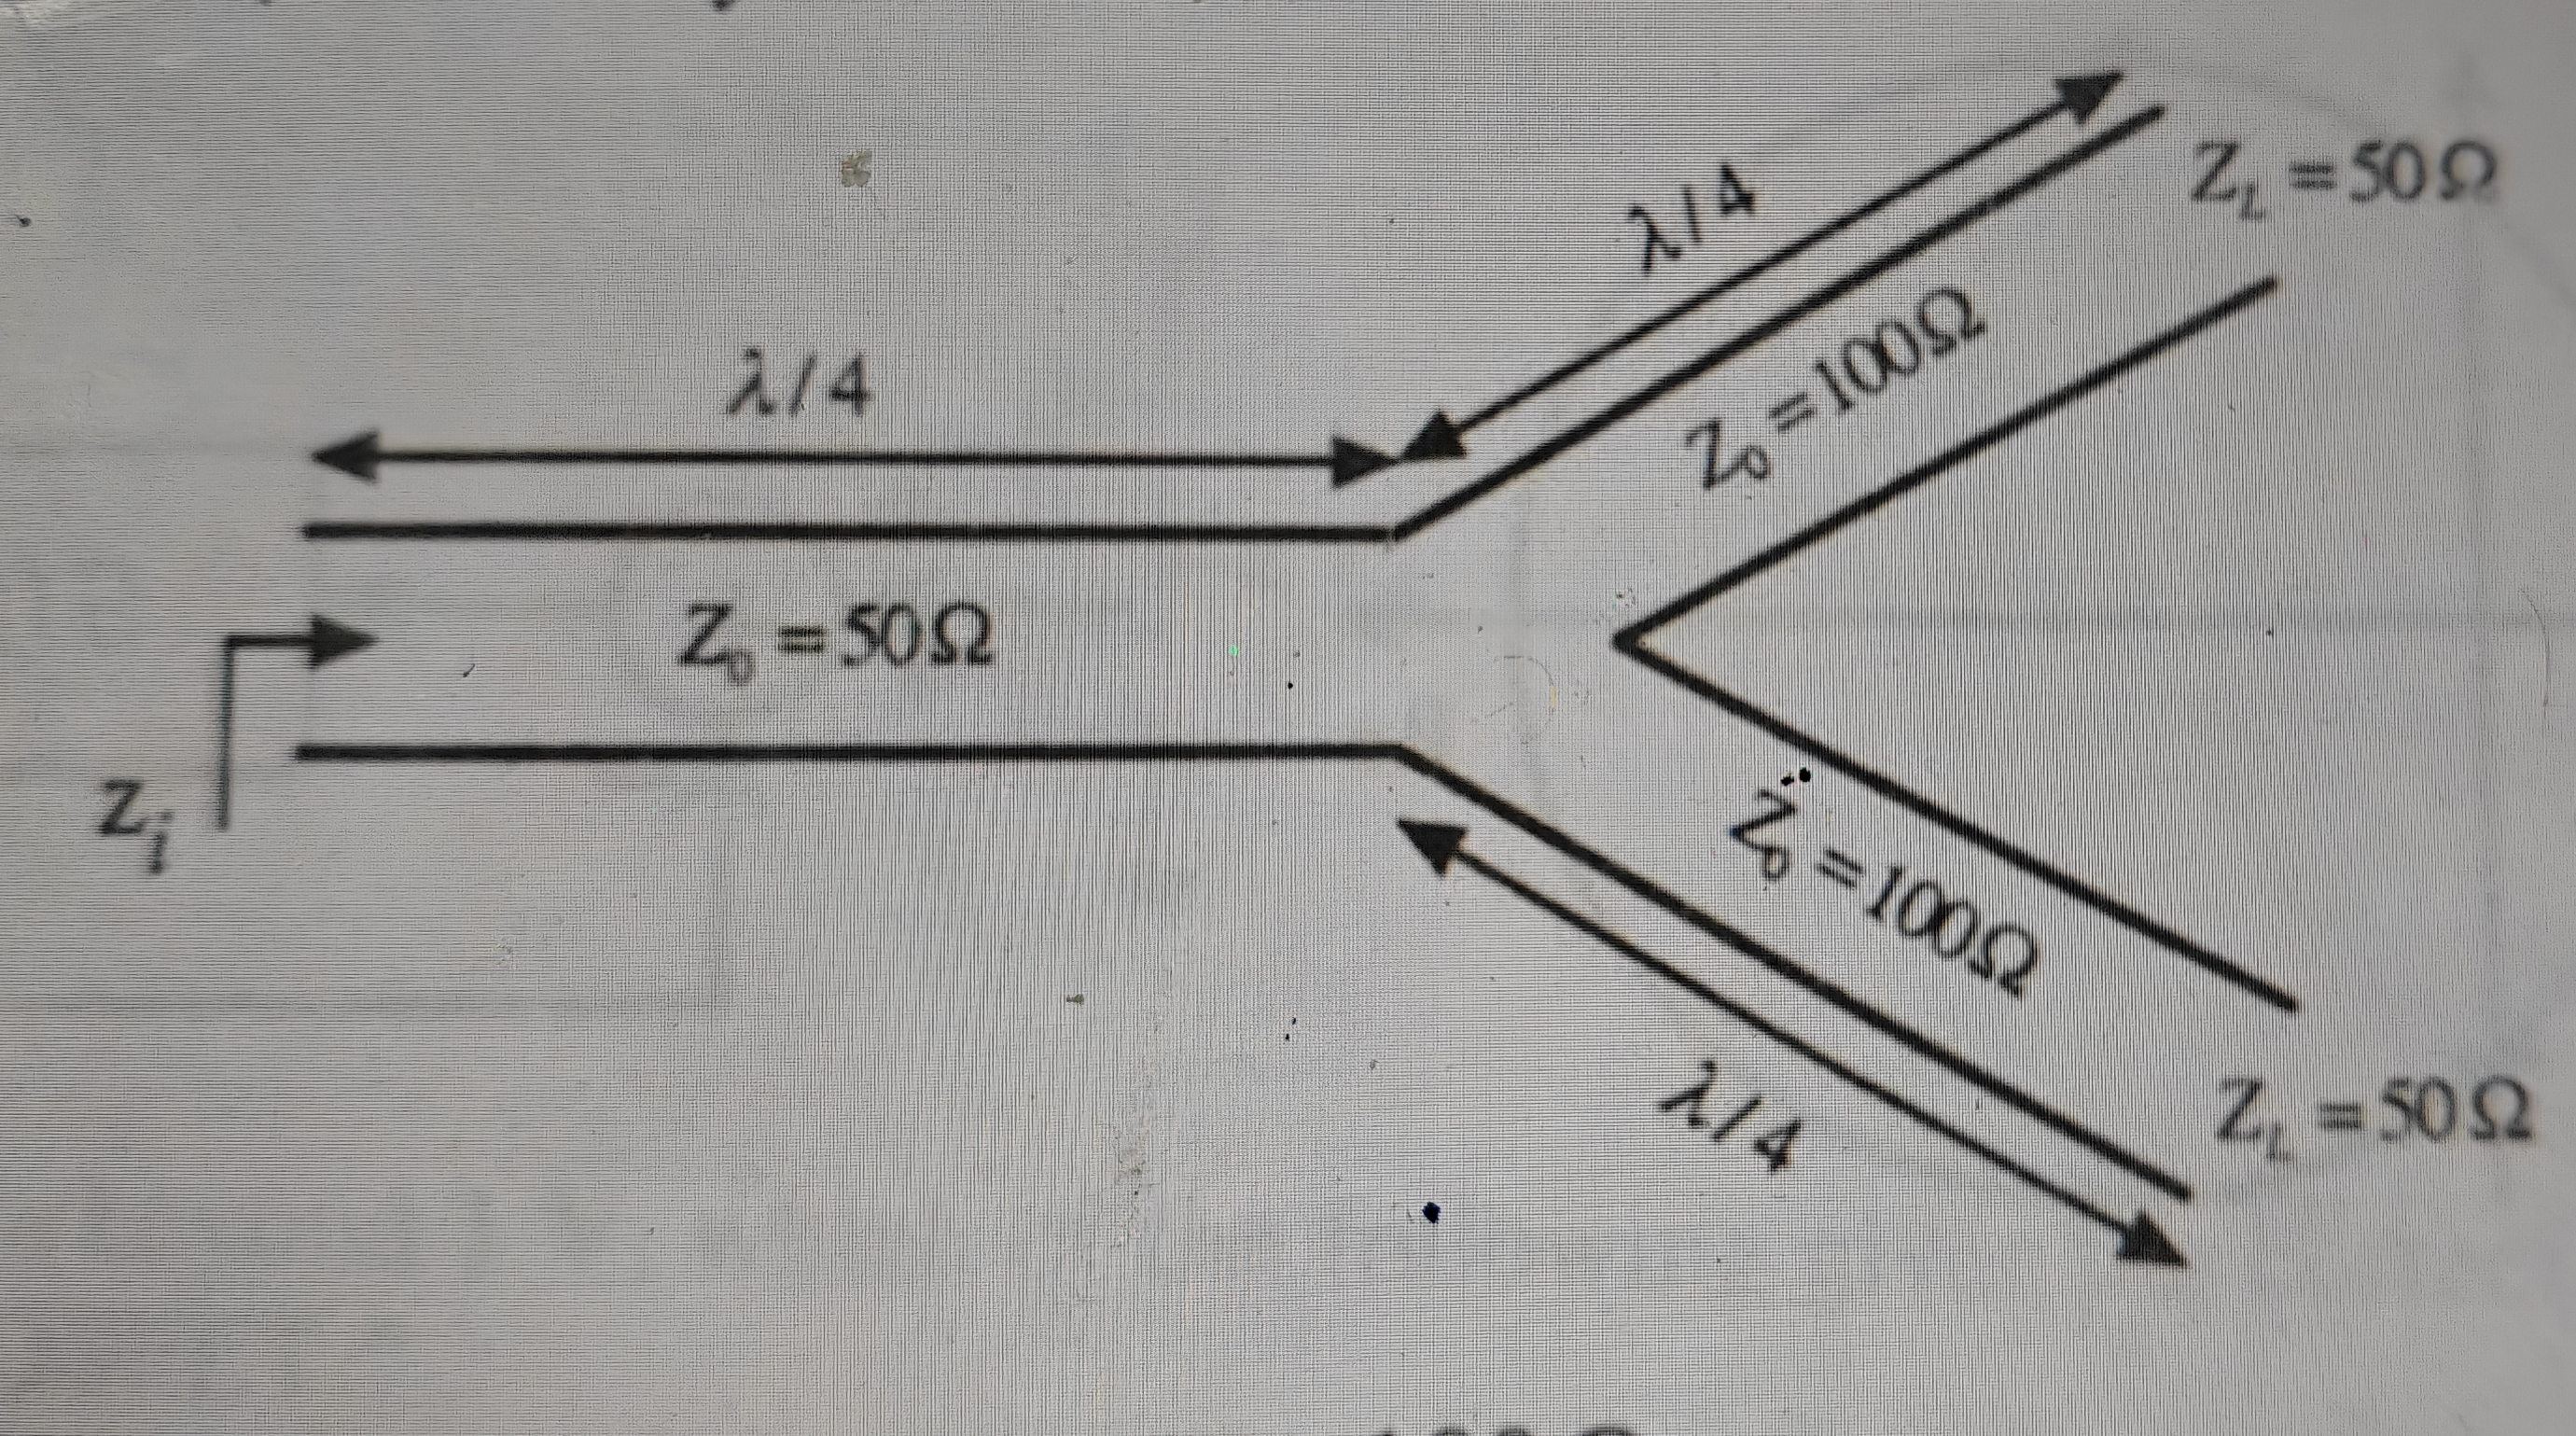
\includegraphics[width=0.5\columnwidth]{figs/fig_21.jpg}
    \caption{\centering Figure for Q-50}
    \label{fig:placeholder_20}
\end{figure}
\begin{enumerate}
    \begin{multicols}{2}
        \item $200 \ohm$
        \item $100 \ohm$
        \item $50 \ohm$
        \item $25 \ohm$
    \end{multicols}
\end{enumerate}
\hfill $\brak{\text{GATE EC 2009}}$

\textbf{Common Data Questions}

for q51 and q52

Consider a silicon p-n junction at room temperature having the following parameters:

Doping on the n-side = $1 x 10^{17} cm^{-3}$

Depletion width on the n-side =$ 0.1 \mu m $

Depletion width on the pride = $1.0 \mu m $

Intrinsic carrier concentration = $1.4 x 10^{10} cm^{-3} $

Thermal voltage = 26 mV 

Permittivity of free space =$8.85 x 10^{-14 }F \cdot cm^{-1} $

Dielectric constant of silicon = 12
\item The built-in potential of the junction is 
\begin{enumerate}
    \begin{multicols}{2}
        \item 0.70 V
        \item 0.76 V
        \item 0.82 V
        \item cannot be estimated from the given data
    \end{multicols}
\end{enumerate}
\hfill $\brak{\text{GATE EC 2009}}$

\item The peak electric field in the device is
\begin{enumerate}
        \item $0.15 MV\cdot cm^{-1}$, directed from p-region to n-region
        \item $0.15 MV\cdot cm^{-1}$, directed from n-region to p-region
        \item $1.80  MV\cdot cm^{-1}$, directed from p-region to n-region
        \item $1.80 MV\cdot cm^{-1}$, directed from n-region to p-region
\end{enumerate}
\hfill $\brak{\text{GATE EC 2009}}$

for q53 and q54

The Nyquist plot of a stable transfer function $G\brak{s}$ is shown in the figure. We are interested in the stability of closed loop system in the feedback configuration shown in the $\figref{fig:placeholder_21}$. 
\begin{figure}[H]
    \centering
    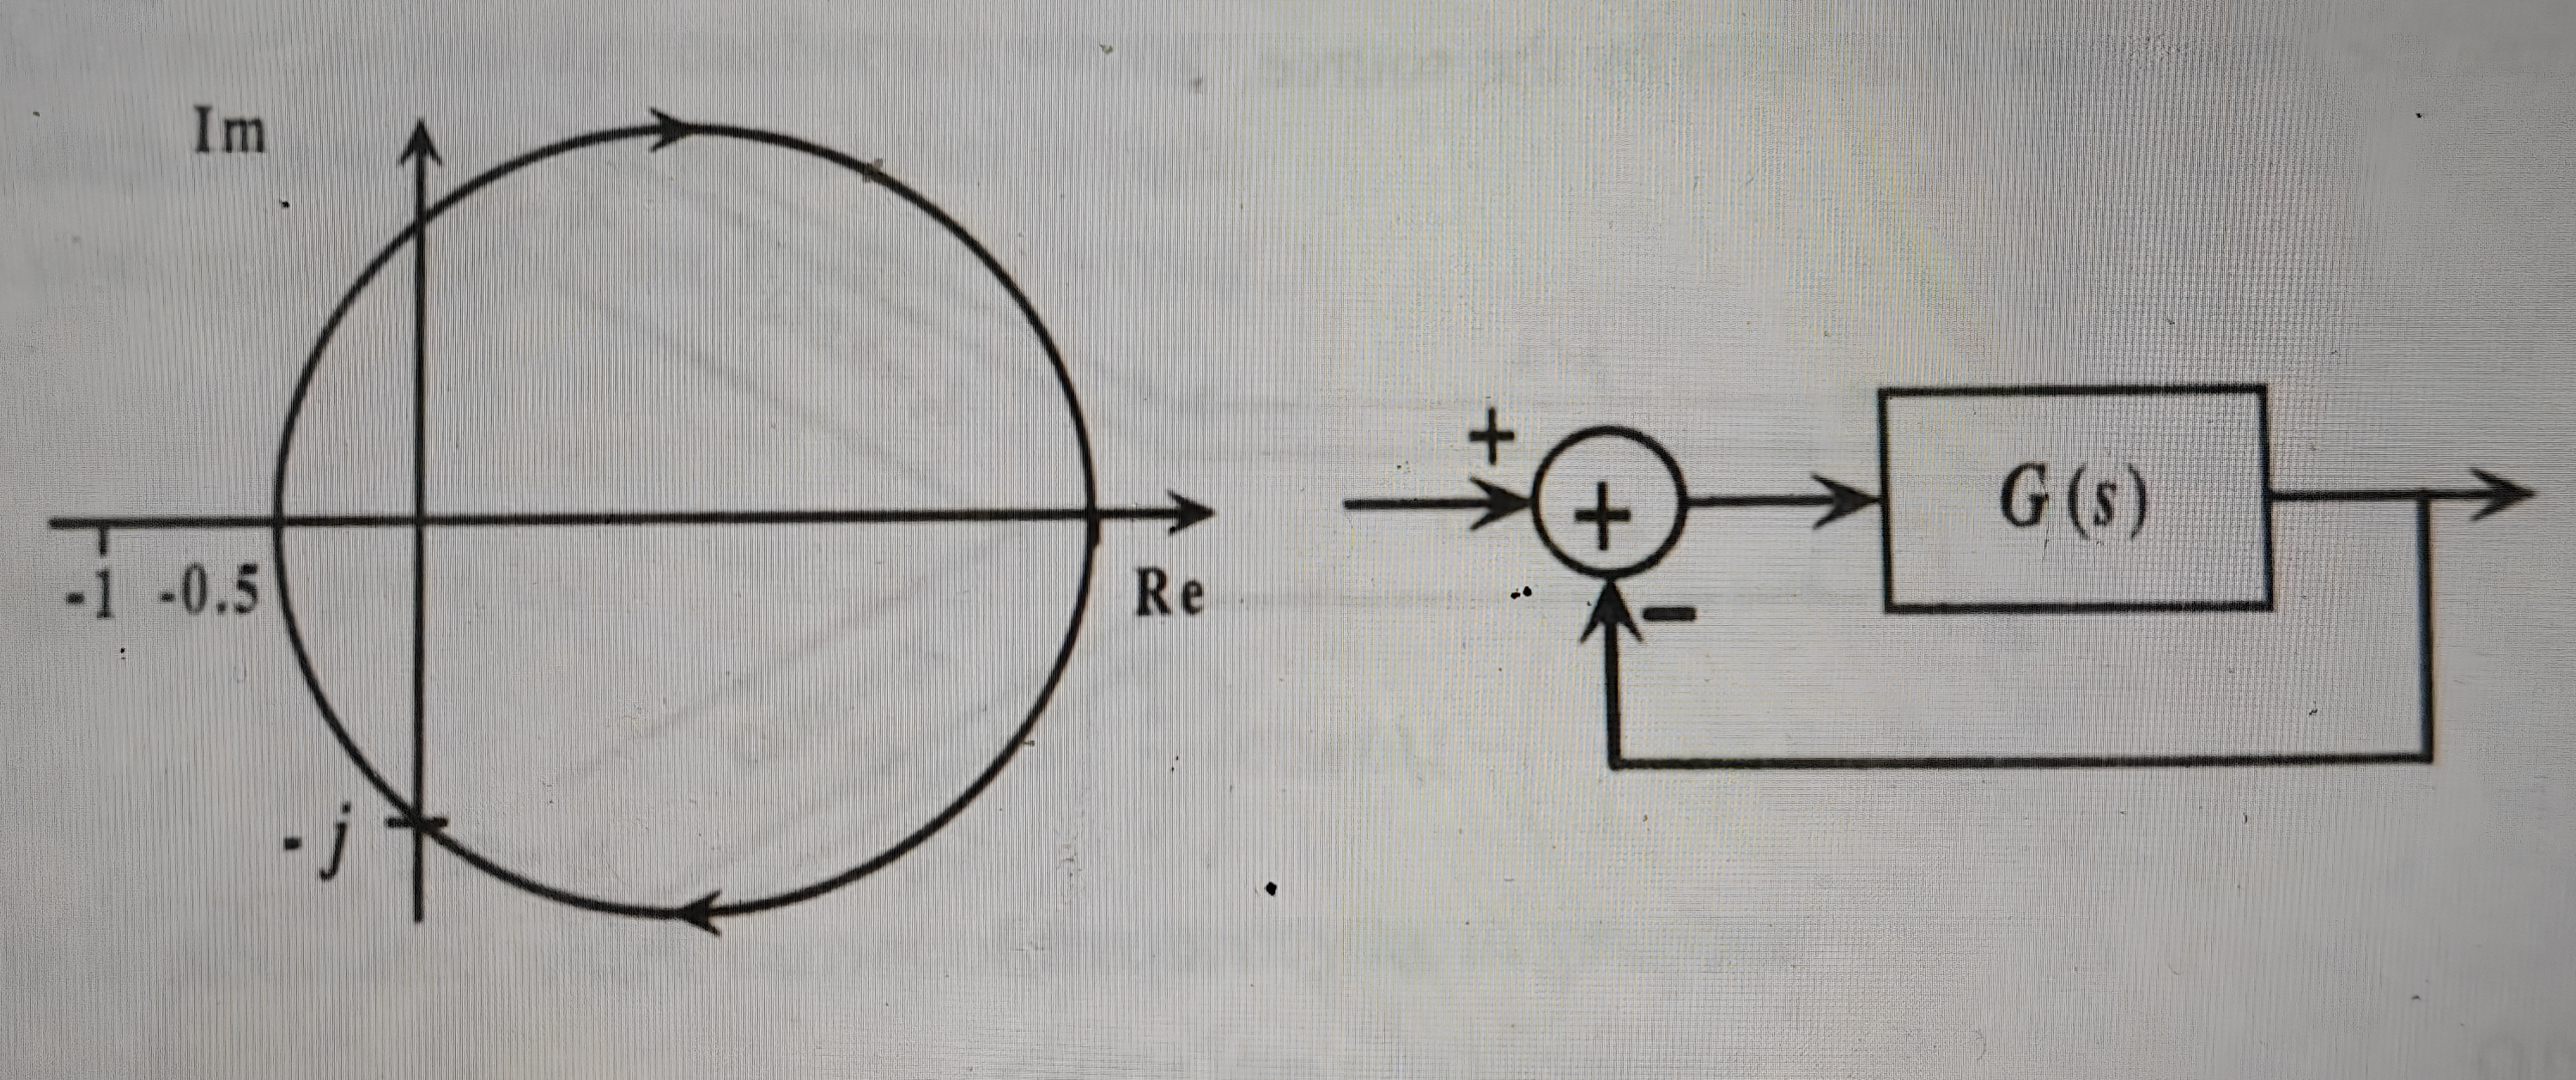
\includegraphics[width=0.5\columnwidth]{figs/fig_22.jpg}
    \caption{\centering Figure for Q-53 and Q-54}
    \label{fig:placeholder_21}
\end{figure}

\item Which of the following is true ?
\begin{enumerate}
    \begin{multicols}{2}
        \item $G\brak{s}$ is an all pass-filter
        \item $G\brak{s}$ has a zero in the right-half plane
        \item $G\brak{s}$ is the impedance of a passive network
        \item $G\brak{s}$ is marginally stable
    \end{multicols}
\end{enumerate}
\hfill $\brak{\text{GATE EC 2009}}$

\item The gain and phase margins of $G\brak{s}$ for closed loop stability are
\begin{enumerate}
    \begin{multicols}{4}
        \item 6 dB and $180^{\degree}$
        \item 3 dB and $180^{\degree}$
        \item 6 dB and $90^{\degree}$
        \item 3 dB and $90^{\degree}$
    \end{multicols}
\end{enumerate}
\hfill $\brak{\text{GATE EC 2009}}$

for q55 and q56 

The amplitude of a $\textbf{random}$ signal is uniformly distributed between $-5V$ and $5V$.

\item If the signal to quantization noise ratio required in uniformly quantizing the signal is $43.5 dB$, the step size of the quantization is approximately 
\begin{enumerate}
    \item $0.0333 V$
    \item $0.05 V$
    \item $0.0667 V$
    \item $0.10 V$
\end{enumerate}

\item If the positive values of the signal are uniformly quantized with a step size of $0.05 V$, and the negative values are uniformly quantized with a step size of $0.1 V$, the resulting signal to quantization noise ratio is approximately 
\begin{enumerate}
    \item $46 dB$
    \item $43.8 dB$
    \item $42 dB$
    \item $40 dB$
\end{enumerate}

for q57 and q58

Consider the CMOS circuit shown in the $\figref{fig:placeholder_23}$, where the gate voltage $v_{c}$ of the n-MOSFET is increased from zero, while the gate voltage of the p-MOSFET is kept constant at $3 V$. Assume that, for both transistors, the magnitude of the threshold voltage is 1 V and the product of the transconductance parameter and the $\brak{W/L}$ ratio, i.e. the quantity $\mu C_{ox} \brak{W/L}$ , is 1 $mA \cdot V^{-2}$
\begin{figure}[H]
    \centering
    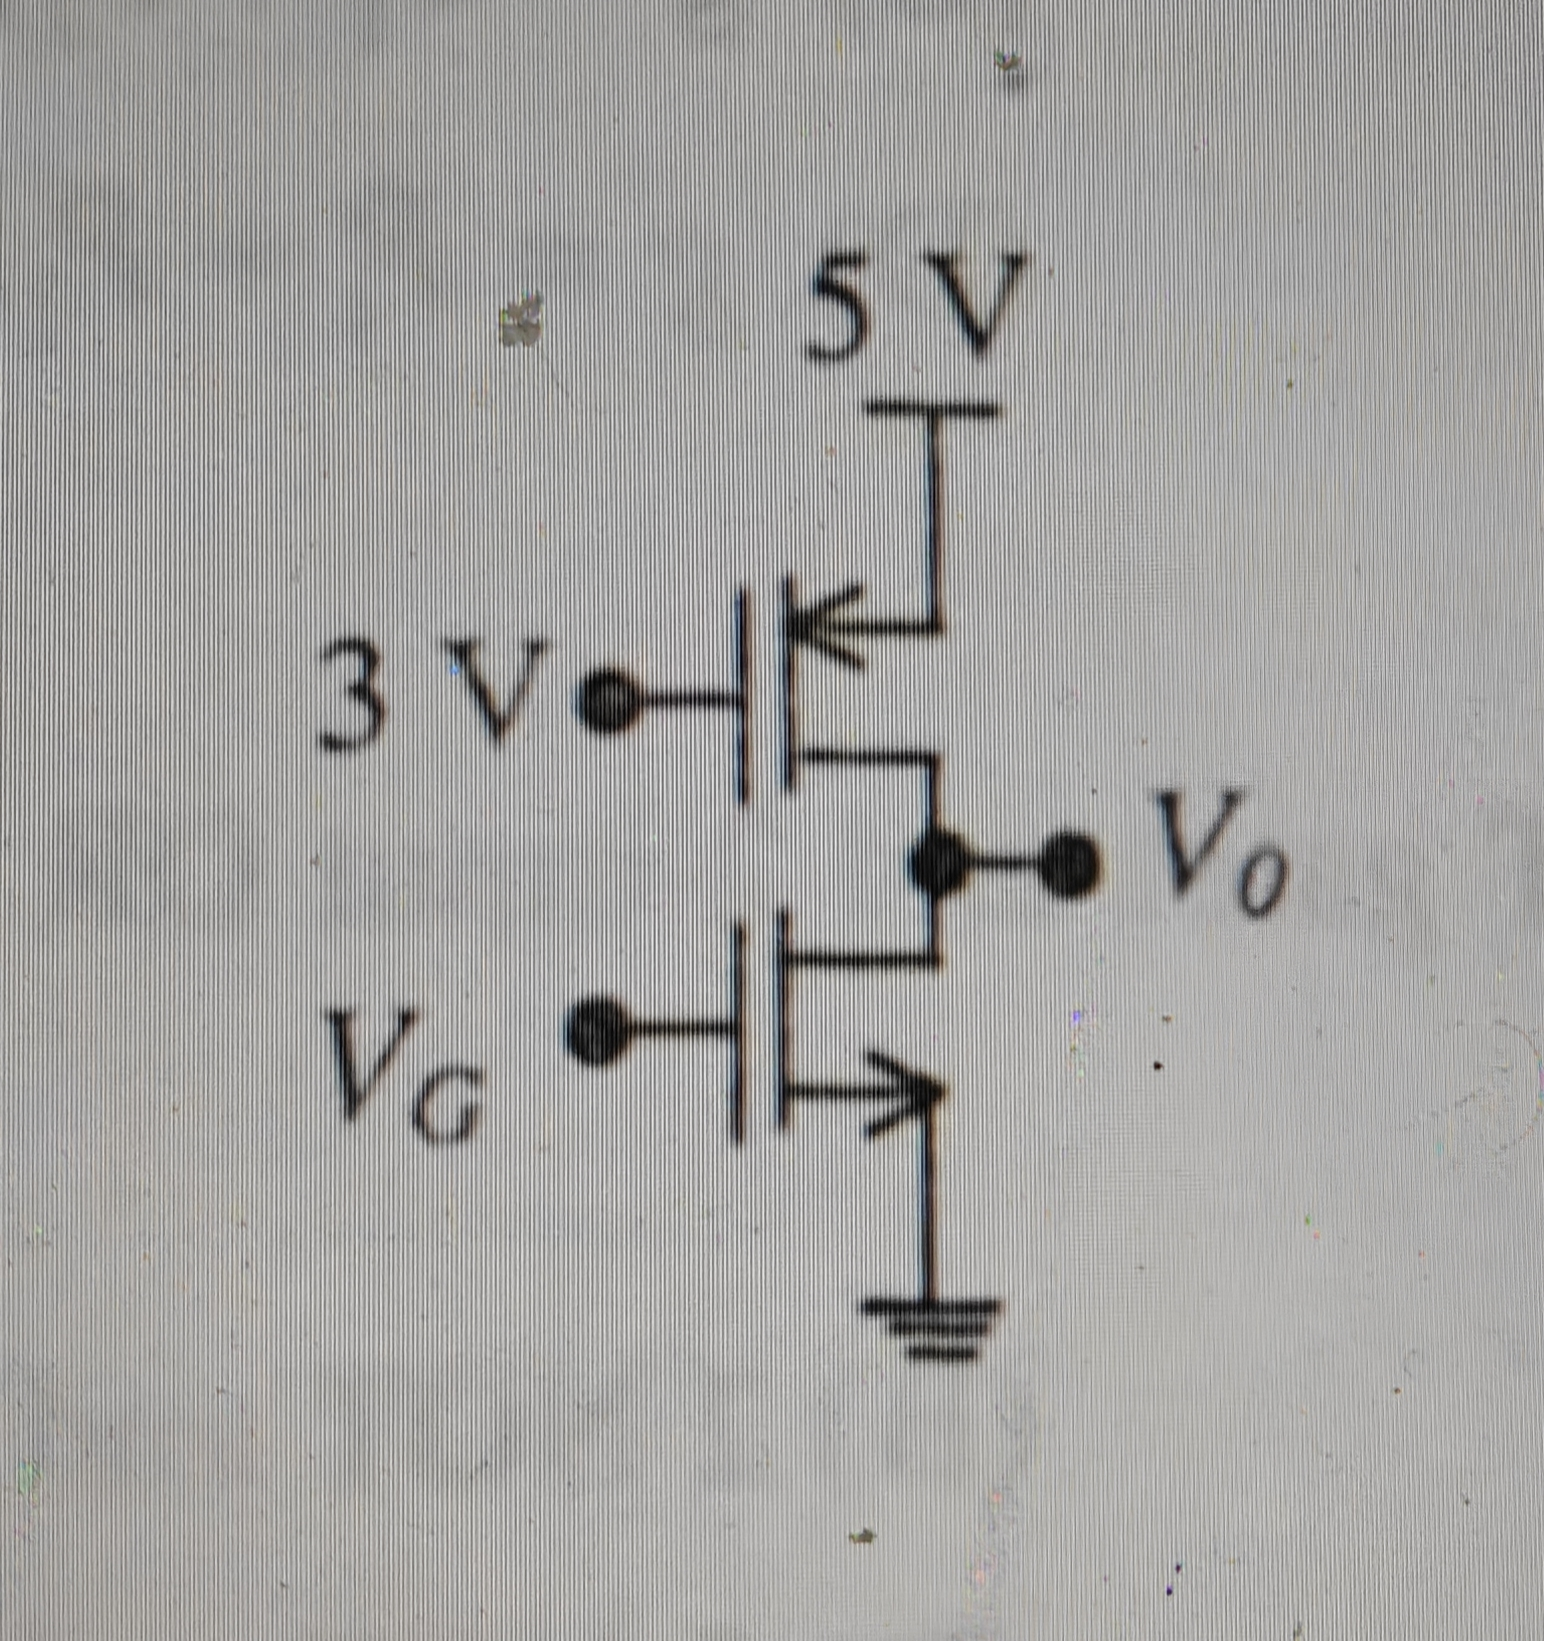
\includegraphics[width=0.5\columnwidth]{figs/fig_23.jpg}
    \caption{\centering Figure for Q-57 and Q-58}
    \label{fig:placeholder_22}
\end{figure}

\item For small increase in $V_G$ beyond 1 V, which of the following gives the correct description of the region of operation of each MOSFET ?
\begin{enumerate}
    \item Both the MOSFETs are in saturation region
    \item Both the MOSFETs are in triode region
    \item n-MOSFET is in triode and p-MOSFET is in saturation region
    \item n-MOSFET is in saturation and p-MOSFET is in triode region
\end{enumerate}

\item Estimate the output voltage $V_o$ for $V_G$ = $1.5V$.
\begin{enumerate}
    \begin{multicols}{4}
        \item $4-\frac{1}{\sqrt{2}}$
        \item $4+\frac{1}{\sqrt{2}}$
        \item $4-\frac{\sqrt{3}}{{2}}$
        \item $4+\frac{\sqrt{3}}{{2}}$
    \end{multicols}
\end{enumerate}
\hfill $\brak{\text{GATE EC 2009}}$

for q59 and q60

Two products are sold from a vending machine, which has two push buttons $P_1$ and $P_2$. When a button is pressed, the price of the corresponding product is displayed in a 7-segment display.
\begin{itemize}

    \item If no buttons are pressed, '0' is displayed, signifying 'Rs. 0'.

    \item If only $P_1$ is pressed, '2' is displayed, signifying 'Rs. 2'.

    \item If only $P_2$ is pressed, '5' is displayed, signifying 'Rs. 5'.

    \item If both $P_1$ and $P_2$ is pressed, 'E' is displayed, signifying 'Error'.
\end{itemize}

The name of the segments in the 7-segment display, and the glow of the display for '0', '2', '5' and 'E', are shown below in the $\figref{fig:placeholder_23}$. 
\begin{figure}[H]
    \centering
    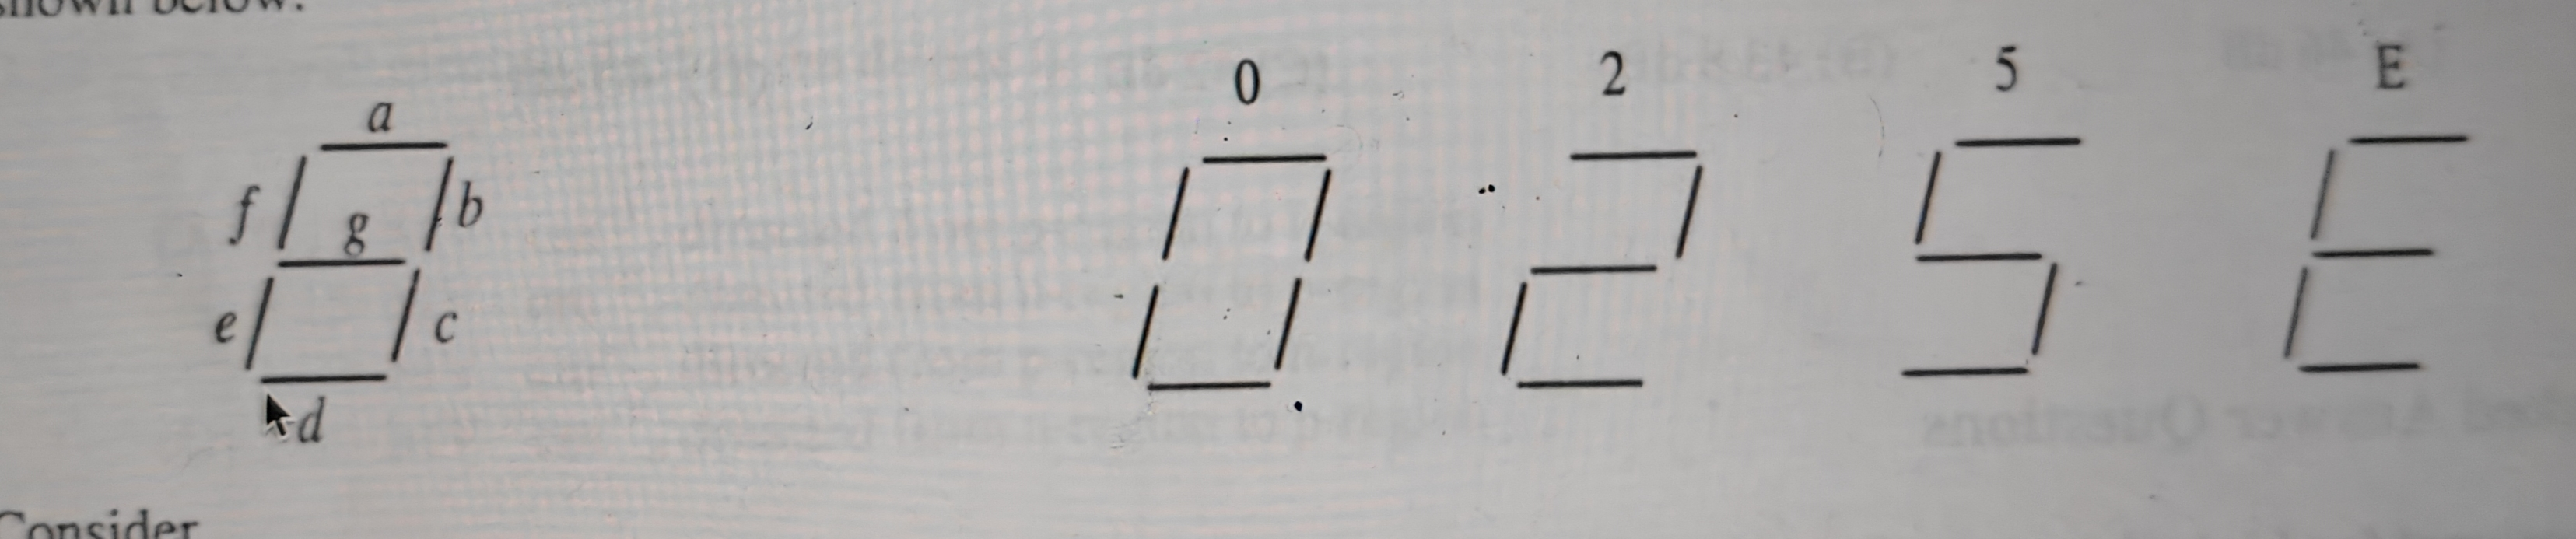
\includegraphics[width=0.5\columnwidth]{figs/fig_24.jpg}
    \caption{\centering Figure for Q-59 and Q-60}
    \label{fig:placeholder_23}
\end{figure}

Consider
\begin{enumerate}
\item push button pressed/not pressed is equivalent to logic 1/10 respectively,

\item a segment glowing/not glowing in the display is equivalent to logic 1/0 respectively.
\end{enumerate}
\item If the segment a to g are considered as functions of $P_1$ and $P_2$, then which of the following is correct?
\begin{enumerate}
    \begin{multicols}{2}
        \item g = $\overline{P_1} + P_2 $, $d=c+e$
        \item g = ${P_1} + P_2 $, $d=c+e$
        \item g = $\overline{P_1} + P_2 $, $e=b+c$
        \item g = ${P_1} + P_2 $, $e=b+c$
    \end{multicols}
\end{enumerate}
\hfill $\brak{\text{GATE EC 2009}}$

\item What are the minimum numbers of NOT gates and 2-input OR gates required to design the logic of the driver for this 7-segment display?

\begin{enumerate}
    \begin{multicols}{2}
        \item 3 NOT and 4 OR
        \item 2 NOT and 4 OR
        \item 1 NOT and 3 OR
        \item 2 NOT and 3 OR
    \end{multicols}
\end{enumerate}
\hfill $\brak{\text{GATE EC 2009}}$
\end{enumerate}
\end{document}